\documentclass[UTF8,a4paper,12pt,fontset=windows]{ctexart}
\usepackage[left=2.7cm,right=2.7cm,top=2.5cm,bottom=2.5cm]{geometry}
\usepackage{fontspec}
\setmainfont{Times New Roman}
\usepackage{amsmath,amssymb,mathtools,bm}
\usepackage{graphicx}
\usepackage{xcolor}
\usepackage{booktabs,longtable,array,multirow,calc}
\usepackage{caption}
\usepackage{float}
\usepackage{setspace}
\usepackage{etoolbox}
\usepackage{titlesec}
\usepackage{url}
\usepackage[hidelinks]{hyperref}

\newcommand{\real}[1]{#1}
\newcounter{none}
\providecommand{\tightlist}{\setlength{\itemsep}{0pt}\setlength{\parskip}{0pt}}
\providecommand{\pandocbounded}[1]{#1}
\newcommand{\hl}[1]{#1}
\setcounter{secnumdepth}{-1}
\setlength{\parindent}{2em}
\setlength{\parskip}{0.25em}
\setlength{\tabcolsep}{4pt}
\renewcommand{\arraystretch}{1.18}
\setstretch{1.45}
\setlength{\LTleft}{0pt}
\setlength{\LTright}{0pt}
\AtBeginEnvironment{longtable}{\small\setstretch{1.12}}
\captionsetup{font=small,labelformat=empty,justification=centering}
\titleformat{\paragraph}[block]{\large\bfseries}{}{0pt}{}
\titlespacing*{\paragraph}{0pt}{1.25ex}{0.6ex}
\ctexset{
  section={format=\Large\bfseries,beforeskip=1.8ex,afterskip=1.0ex},
  subsection={format=\large\bfseries,beforeskip=1.5ex,afterskip=0.8ex},
  subsubsection={format=\normalsize\bfseries,beforeskip=1.2ex,afterskip=0.6ex}
}
\emergencystretch=3em

\begin{document}
\pagestyle{plain}
\begin{center}
  {\zihao{2}\bfseries 农业全要素生产率对经济高质量发展的驱动\par}
  \vspace{0.8em}
  {\zihao{2}\bfseries 机制与空间效应\par}
\end{center}
\vspace{1.5em}
\noindent\textbf{摘要：}\par
\noindent\textbf{关键词：}\par
\vspace{1em}
\section{1引言}\label{ux5f15ux8a00}

根据国家统计局提供的相关数据，我国截止2025年末，总人口数为14.0489亿，作为人口大国与之相配的农业发展至关重要并与经济发展、人民生活质量的提高密切相关。2025年和2024年国内生产总值增长 (百分点)皆为5.0，2023年则为5.4，其中第一产业对国内生产总值增长的拉动 (百分点)仅占0.3，第一产业近三年对GDP的贡献率 (\%)也远远不及第二、第三产业，其平均约为5.6\%。可以发现其对经济发展的贡献还有极其广泛的增长空间，在追寻高质量发展的今天，农业全要素生产率（Agricultural Total Factor Productivity，简称农业TFP）针对此类问题为我们的研究提供了不同于传统的新路径，即能否通过农业全要素生产率的提升来提高农业产出进而推动经济的高质量发展，基于此，本研究将从宏观视角出发采用省级面板数据结合空间计量经济学的思想深刻探讨农业全要素生产率对经济发展的驱动机制与空间效应。

\section{2文献综述}\label{ux6587ux732eux7efcux8ff0}

\subsection{2.1经济高质量发展的相关研究}\label{ux7ecfux6d4eux9ad8ux8d28ux91cfux53d1ux5c55ux7684ux76f8ux5173ux7814ux7a76}

\subsubsection{（一）概念研究}\label{ux4e00ux6982ux5ff5ux7814ux7a76}

经济高质量发展由习近平总书记在党的十九大报告中指出首次正式提出的新表述。之后我国各学者随即开始对其的研究，在后续的官方定义中明确将其与经济增长判定为两个不同的概念。经济发展是指量的增长和质的提升，是量和质的有机统一。 (《经济日报》, 2023)

其主要内容包括：构建高水平社会主义市场经济体制、建设现代化产业体系、全面推进乡村振兴、促进区域协调发展、推进高水平对外开放几大内容

\subsubsection{（二）过往研究}\label{ux4e8cux8fc7ux5f80ux7814ux7a76}

较早的一批研究中蒲晓晔; {[}奥{]} Jarko Fidrmuc从动力结构出发以优化供求侧、结构来构建新常态经济发展的动力体系促进经济高质量发展 (蒲晓晔, 以及其他人, 2018)，陈诗一，陈登科站在环境保护和政府治理探究雾霾污染对中国经济发展质量的影响及其传导机制， (陈诗一，陈登科, 2018)，师博、任保平以增长的基本面和社会成果两个维度来对中国省际经济高质量发展指标体系进行构建与测算 (中国省际经济高质量发展的测度与分析, 2018年)

在高质量发展提出之前，经济学界普遍采用经济增长质量来讨论经济增长 ``质''的问题 (陈景华, 以及其他人, 2020)

我们通常认为的国民生产总值（GDP）其实质更偏向于经济增长的量概念而不是经济发展质的概念也就无法进一步较为准确的判定经济高质量增长这一被解释变量，针对国民生产总值（GDP）无法完全对经济高质量增长这一解释变量完美适配这一问题，现有研究中陈诗一、陈登科采用了人均国民生产总值作为被解释变量表示经济发展 (陈诗一，陈登科, 2018)赵涛通过设定包括产业结构等在内的5个二级指标构成的多维评价体系，通过一系列测算得到高质量发展水平 (赵涛, 2020)，蔡文新等则通过熵权法从``创新、协调、绿色、开放、共享''五个维度构建了经济高质量发展指标体系 (科技金融、经营主体活力与经济高质量发展, 2026)为我们扩展经济发展的界定指标提供了新的思路可以将其经济增长的``质''属性放大与新质生产力相关联来摆脱经济增长单纯的量扩张，而赵丽芳等提出依据新发展理念的五个维度---创新、协调、绿色、开放、共享，构建高质量发展评价指标体系是国内主流做法 (赵丽芳, 2026)其提出的以创新、协调、绿色、开放、共享为一级指标，细化设计12个二级指标和21个三级指标，构建经济高质量发展评价指标体系，运用熵值法构建高质量发展指数的方法进一步证明了以多维评价构建经济高质量发展综合指数的可能性。

本研究正是基于主流方法以创新、协调、绿色、开放、共享为核心思想构建经济高质量发展综合指数。

\subsection{2.2研究假说与创新}\label{ux7814ux7a76ux5047ux8bf4ux4e0eux521bux65b0}

\subsubsection{2.2.1研究假说}\label{ux7814ux7a76ux5047ux8bf4}

20世纪中叶，巴顿和库珀（Barton \& Cooper）率先将全要素生产率概念应用于农业生产研究，是综合测度农业经济效率的理论范畴和统计指标，其本质与一般的``全要素生产率''的定义是相同。

农业全要素生产率作为本文的解释变量，其本身根据肯德里克的定义可表述为农业总产出与综合投入（包括土地、资本、劳动和中间投入等因素）的比值，其核心思想在于排除传统要素投入所带来的影响后，通过技术进步、制度调整优化、资源整合分配等非传统因素提升生产效率与五大新发展理念中的``创新维度''密不可分，而创新作为本文构建高质量发展指数的重要部分所以除了传统解释变量对被解释变量的解释效应之外可能存在着被解释变量对解释变量的反向解释作用，基于此，本研究做出了假设一：

H1：农业全要素生产对经济发展起到显著的推动作用且与经济高质量发展之间存在相互支撑、相互耦合的双向互动关系。（耦合协调度）

农业TFP的提高同农业领域内的资源配置效率有显著的关系 (技术效率、技术进步与中国农业全要素生产率的提高------基于国际比较的实证分析, 2010)，生产率高值集聚区域由最初东北、华北、华东、华中、西南、西北局部点状集聚，逐步向东南沿海与北方、西南外围拓展，呈现全域广域分布空间格局。(绿色技术创新对农业绿色全要素生产率影响的异质性与机制研究, 2026)

刘溪、梁雪涵也指出中国四大区域的农业要素生产率呈现明显的``东部\textgreater 西部\textgreater 中部\textgreater 东北''的特征。 (中国农业全要素生产率时空格局、动态演进与影响因素研究, 2026)且从全国范围来看，农业全要素生产率增长表现出地区之间增长的不平衡性且差距表现有扩大的趋势。 (我国农业全要素生产率分解及其区域发展不平衡分析, 2020)

不难发现，农业全要素生产率已有的明显空间发展格局以及相应的空间计量思想，故本研究做出了假设二至假说五：

H2：耦合协调度在空间上呈现显著的聚集特征，且总体差距主要来源于区域间差异，分布成多极化演变趋势（莫兰、Dagum基尼系数、核密度）

H3：影响协调度的各因素不仅存在本地直接效益，还通过空间传导对邻近地区产生显著的间接溢出效应（空间溢出）

H4：核心驱动因素对耦合协调度的影响存在基于经济发展水平的门槛效应，成非线性转化特诊。（门槛效应）

H5：在现有的空间溢出与门槛机制下，耦合协调度的状态转移具有较强稳定性，低水平省份向上跃迁的概率较低，存在``等级锁定''风险。（马尔科夫链）

\subsubsection{2.2.2指标构建创新}\label{ux6307ux6807ux6784ux5efaux521bux65b0}

\paragraph{2.2.2.1高质量发展综合指数（Y）构建}\label{ux9ad8ux8d28ux91cfux53d1ux5c55ux7efcux5408ux6307ux6570yux6784ux5efa}

本研究以五大新发展理念为基础，考虑到后续农业全要素生产率测算中部分农业指标数据的部分空缺，我们收集了数据较为完善的31个省级行政区（不包含港澳台）从2016到2020共5年的16项二级评价指标，依据指标经济内涵与属性特征，归类分入五大一级评价指标，通过五大一级指标来对五大新发展理念进行表述、实现对高质量发展综合指数表达。

\begin{longtable}[]{@{}
  >{\centering\arraybackslash}p{(\linewidth - 6\tabcolsep) * \real{0.4419}}
  >{\raggedright\arraybackslash}p{(\linewidth - 6\tabcolsep) * \real{0.2366}}
  >{\raggedright\arraybackslash}p{(\linewidth - 6\tabcolsep) * \real{0.1608}}
  >{\centering\arraybackslash}p{(\linewidth - 6\tabcolsep) * \real{0.1608}}@{}}
\caption{表格 1经济高质量发展指标选取}\tabularnewline
\toprule\noalign{}
\begin{minipage}[b]{\linewidth}\centering
\textbf{一级指标}
\end{minipage} & \begin{minipage}[b]{\linewidth}\centering
\textbf{二级指标}
\end{minipage} & \begin{minipage}[b]{\linewidth}\centering
\textbf{负向指标}
\end{minipage} & \begin{minipage}[b]{\linewidth}\centering
\textbf{正向指标}
\end{minipage} \\
\midrule\noalign{}
\endfirsthead
\toprule\noalign{}
\begin{minipage}[b]{\linewidth}\centering
\textbf{一级指标}
\end{minipage} & \begin{minipage}[b]{\linewidth}\centering
\textbf{二级指标}
\end{minipage} & \begin{minipage}[b]{\linewidth}\centering
\textbf{负向指标}
\end{minipage} & \begin{minipage}[b]{\linewidth}\centering
\textbf{正向指标}
\end{minipage} \\
\midrule\noalign{}
\endhead
\bottomrule\noalign{}
\endlastfoot
\multirow{4}{=}{\centering\arraybackslash 经济运行质效（Economic Development Quality \& Efficiency,Dev\_Qual）} & PCGDP(人均地区生产总值) & & PCGDP \\
& PCRS（人均社会消费品零售额） & & PCRS \\
& TIG（第三产业增加值增长率） & & TIG \\
& HBTP（高技术产业主营业务收入占比） & & HBTP \\
\multirow{2}{=}{\centering\arraybackslash 政府经济治理(Government Governance Effectiveness,Gov\_Eff)} & FSG（财政自给率） & & FSG \\
& GCR（政府消费率） & & GCR \\
\multirow{4}{=}{\centering\arraybackslash 城乡区域均衡（Urban-Rural Coondinated Development,UrbRur\_Coor）} & IPR（常住人口城镇化率） & & IPR \\
& RUUR（城乡收入比） & RUUR & \\
& PCURA（人均城市道路面积） & & PCURA \\
& PTVP(每万人拥有公共交通车辆) & & PTVP \\
\multirow{3}{=}{\centering\arraybackslash 生态绿色可持续

（Green \& Low-Carbon Development,Green\_LowC）} & WEI（每单位GDP能耗） & WEI & \\
& SDEI（单位GDP污染物排放程度） & SDEI & \\
& EPES（电力消费弹性系数） & EPES & \\
\multirow{3}{=}{\centering\arraybackslash 居民民生福祉

（Shared Development \& Social Welfare,Share-Welf）} & HESP（人均医疗卫生财政支出） & & HESP \\
& UGPR（城市燃气普及率） & & UGPR \\
& UWPR（城市用水普及率） & & UWPR \\
\end{longtable}

（1）非线性检验：Spearman秩相关系数（\(\rho\)）

传统熵权法未考虑指标间的相关性，经典CRITIC依赖皮尔逊相关仅适用于线性关联场景。本研究采用Spearman秩相关系数替代皮尔逊系数改进CPITIC模型。具体是将原始数据\(x_{i}\)、 \(y_{i}\)分别替换为各自的秩次（1，2，3\ldots，n）即排名等级：\(R\left. (x_{i} \right.),R\left. (y_{i} \right.)\)并按升序排再对两指标的秩次序列计算Pearson相关系数。若两指标的秩次同步上升或下降，即使变动幅度非线性，其Pearson系数仍趋近于1，从而有效捕捉指标间的非线性单调关联

\[\begin{array}{r}
\rho = \frac{\sum_{i = 1}^{n}{\left( R\left( X_{i} \right) - \overline{R_{X}} \right)\left( R\left( Y_{i} \right) - \overline{R_{Y}} \right)}}{\sqrt{\sum_{i = 1}^{n}\left( R\left( X_{i} \right) - \overline{R_{X}} \right)^{2} \cdot \sum_{i = 1}^{n}\left( R\left( Y_{i} \right) - \overline{R_{Y}} \right)^{2}}}\qquad(1)
\end{array}\]

符号含义：\(R\left( X_{i} \right)\)为\(X_{i}\)在全体样本中的升序排名，\(\overline{R_{X}}\)为平均秩次。\(R\left( y_{i} \right)\)为\(y_{i}\)在全体样本中的升序排名，\(\overline{R_{y}}\)为平均秩次。

2.非线性诊断

绝对异差（\(Diff\)）为：

\[\begin{array}{r}
\text{Diff} = |r - \rho|\qquad(2)
\end{array}\]

当\(\text{Diff}\)平均值\textless{} 0.1时，整体上数据近似线性。

若存在部分指标对的\(\text{Diff}\)显著较大（例如\textgreater0.2），则说明存在局部非线性单调趋势。

本文实际诊断结果：全样本16个二级指标共120对组合中，平均\(\text{Diff}\)=0.0902，虽整体趋近线性，但存在最大差异对，高达0.3以上。为避免线性假设失效导致权重偏误，本文最终采用Spearman秩相关系数衡量指标冲突性。

（2）CRITICS-spearman-\/-熵权法

1.数据标准化处理

由于表一中各指标的量纲和本身数量上存在的差异，如果不加以处理，正向、负向指标将无法对比，原始数据会干扰后续的赋权与综合评价结果造成综合得分与空间计量结果系统性的偏误，具体过程如下：

\begin{quote}
（1）正向指标：
\end{quote}

\[\begin{array}{r}
y_{ij}' = \frac{\left( x_{ij} - x_{\min} \right)}{\left( x_{\max} - x_{\min} \right)}\qquad(3)
\end{array}\]

其中，\(x_{ij}\):第i个评价对象在第j个正向指标上的原始数据，\(x_{\min}\):第j个正向指标的最小值，\(x_{\max}\):第j个正向指标的最大值，\(y_{ij}'\):标准化后的数据（取值范围在{[}0,1{]}之间，越接近1代表该指标表现更好）

\begin{quote}
（2）负向指标

\[\begin{array}{r}
y_{ij}' = \frac{\left( x_{\max} - x_{ij} \right)}{\left( x_{max} - x_{min} \right)}\qquad(4)
\end{array}\]
\end{quote}

其中，\(x_{ij}\):第i个评价对象在第j个正向指标上的原始数据，\(x_{\min}\):第j个正向指标的最小值，\(x_{\max}\):第j个正向指标的最大值，\(y_{ij}'\):标准化后的数据（取值范围在{[}0,1{]}之间，越接近1代表该指标表现更好）

2.熵权法计算波动性

在完成标准化去除量纲后，首先对各二级指标进行赋权得到对应的一级指标，各一级指标再度赋权最终构成被解释变量经济高质量发展综合指数，信息熵原理：指标的数据离散程度越大，所包含的信息量就越多，权重越高，具体过程如下：

\begin{quote}
（1）评价比重\(p_{ij}\)
\end{quote}

\[\begin{array}{r}
p_{ij} = \frac{y_{ij}}{\sum_{i = 1}^{n}y_{ij}}\qquad(5)
\end{array}\]

其中，\(p_{ij}\)：第j个指标下，第i个样本所占比重,\(y_{ij}\)：第i个样本在第j个指标上的标准化值，\(n\)：样本数量

\begin{quote}
（2）计算指标信息熵\(e_{j}\)
\end{quote}

\[\begin{array}{r}
e_{j} = - k\sum_{i = 1}^{n}{p_{ij}\ln\left( p_{ij} \right)},k = - \frac{1}{ln\ n}\qquad(6)
\end{array}\]

其中ej\(\in\){[}0,1{]}。熵值越大，说明数据愈发混乱、差异越小

（3）计算差异系数（波动性\(d_{j}\)）

\[\begin{array}{r}
d_{j} = 1 - e_{j}\qquad(7)
\end{array}\]

其中，\(d_{j}\)越大，代表该指标自身的波动信息量越大

3.Spearman法计算冲突性\(\delta_{j}\)

进一步是衡量指标间的信息重叠程度

\begin{enumerate}
\item
  计算Spearman相关系数矩阵
\end{enumerate}

\begin{quote}
以标准化矩阵\(y_{ij}'\)，计算第j个指标与第k个指标的秩相关系数
\end{quote}

\[\begin{array}{r}
\rho_{jk} = \frac{\sum_{i = 1}^{n}{\left( R_{ij} - \overline{R_{j}} \right)\left( R_{ik} - \overline{R_{k}} \right)}}{\sqrt{\sum_{i = 1}^{n}\left( R_{ij} - \overline{R_{j}} \right)^{2} \cdot \sum_{i = 1}^{n}\left( R_{ik} - \overline{R_{k}} \right)^{2}}}
\end{array}\]

其中，\(R_{ij}\)为第j个指标下第i个样本的秩次；\(\overline{R_{j}}\)是该指标的平均秩次。

（2）计算冲突性\(\delta_{j}\)

\[\begin{array}{r}
\delta_{j} = \sum_{k = 1}^{m}\left( 1 - \rho_{jk} \right)\qquad(8)
\end{array}\]

其中，当\(\rho_{jk}\)接近1（高度正相关），(\(1 - \rho_{jk}\))接近0，冲突性低，说明信息冗余严重，应压低权重；当\(\rho_{jk}\)接近 0（相关性弱），(\(1 - \rho_{jk}\))接近1，冲突性高，说明该指标具有独特信息，应抬高权重

4.计算综合信息量（\(C_{j}\)）

将波动性与冲突性相乘，得到每一个指标的综合信息承载量

\[\begin{array}{r}
C_{j} = d_{j} \times \delta_{j}\qquad(9)
\end{array}\]

5.计算最终客观权重（\(W_{j}\)）

\[\begin{array}{r}
W_{j} = \frac{C_{j}}{\sum_{j = 1}^{m}C_{j}},\ \text{满足}\sum_{j = 1}^{m}W_{j} = 1\qquad(10)
\end{array}\]

6.计算综合得分（\(S_{i}\)）

将标准化后的数据与权重进行线性加权求和：

\[\begin{array}{r}
S_{i} = \sum_{j = 1}^{m}W_{j} \cdot y_{ij}'\qquad(11)
\end{array}\]

符号含义：\(S_{i}\)为第\(i\)个样本的二级指标得分。

接着对一级指标重复上述过程，完成两阶段赋权得到高质量发展综合指数（Y），具体如下所示：

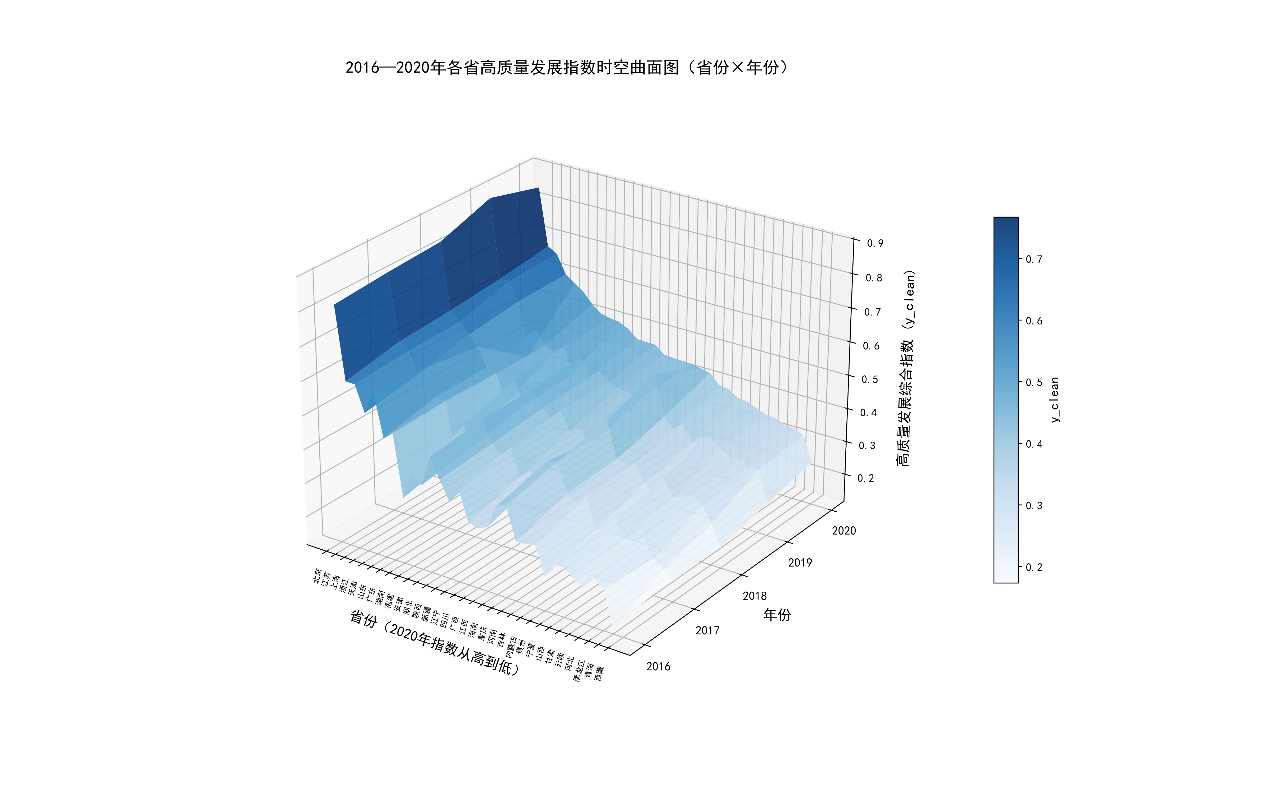
\includegraphics[width=5.76042in,height=3.59931in]{media/media/image1.png}

\emph{\textbf{Figure1：2016\textasciitilde2020年各省级行政区高质量发展综合指数三维曲面图}}

Figure1展示了2016---2020年的各省高质量发展综合指数的三维时空曲面，其中x轴为按2020年指数从高到低排列的省份，y轴为年份，z轴为高质量发展综合指数。从曲面整体走势来看，绝大多数省份的曲面沿年份方向呈现平稳上升态势，表明考察期内我国各省高质量发展水平普遍提升。

从省份截面来看，曲面左边（排名靠前的省份）明显高于右边（排名较后的省份），反映出省际间发展不平衡特征明显。

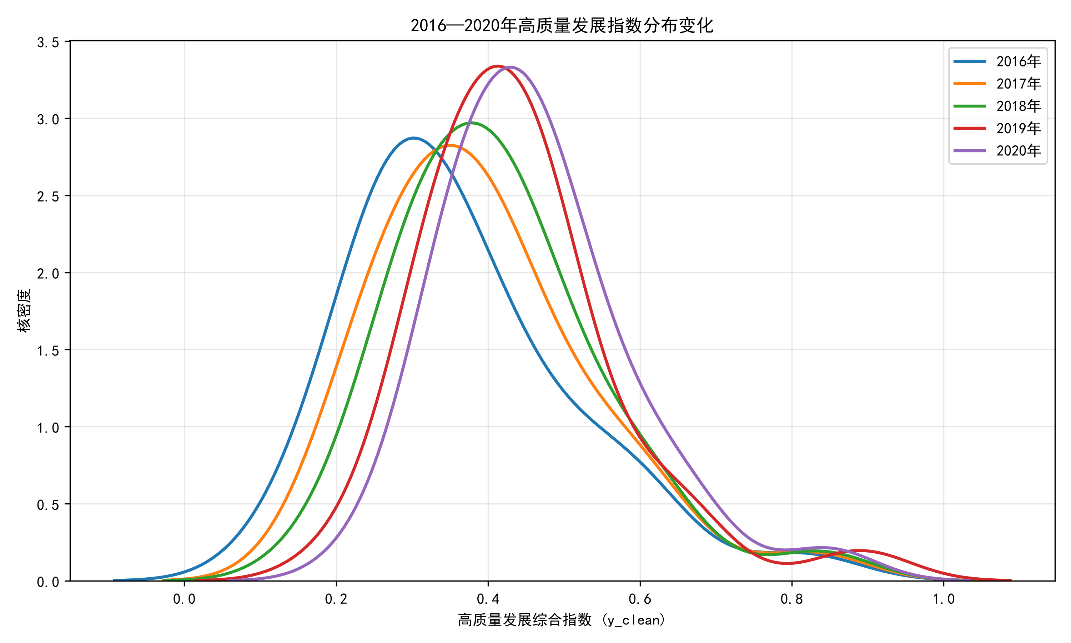
\includegraphics[width=4.86979in,height=2.92023in]{media/media/image2.png}

\emph{\textbf{Figure2：总体核密度图---高质量发展综合指数分布变化}}

Figure2报告了各年度高质量发展综合指数的核密度估计曲线。在这里我们只做简单的分析在后续的统计分析中我们将进一步详细的进行说明，从位置分布来看，密度曲线从2016-2020年持续整体向右移动，表明样本区间高质量发展综合指数我国整体水平逐年提高；而从分布形态上看，曲线的主峰高度随着年份的增加而逐步上升、宽度逐渐收窄，说明各省份的高质量发展综合指数集中程度有所增强，离散程度降低。上述特征说明，在2016-2020年间我国省际高质量发展水平呈现整体提升、差距有所缩小的良好态势。

\paragraph{2.2.2.2农业全要素生产率（x）的构建}\label{ux519cux4e1aux5168ux8981ux7d20ux751fux4ea7ux7387xux7684ux6784ux5efa}

所谓``全要素生产率''就是产量与全部要素投入量的比率 (贵州农业全要素生产率:初步测度与简要分析, 1999)，而农业全要素生产率（TFP）的测度方法主要分为参数法、非参数法和指数法三大类。虽然各有不同，但其核心思想都是从总产出增长中``剔除''所有可观测要素投入（土地、劳动、资本等）的贡献，剩余部分即为TFP的增长。Shenggen Fan等采用了较为经典的索洛残差法（增长核算法） (Production and Productivity Growth in Chinese Agriculture: New National and Regional Measures, 2002)，但该方法假设完全竞争市场和规模报酬不变但如果真实世界的报酬递增农业全要素生产率就会被高估反之则会被低估，故在现实中该假设因为苛刻而难以满足、并且其还存在引起农业全要素增长率的增长因素不明确、数据尤其是要素收入份额（地租、劳动者报酬等）要求准确等问题。

余康等则基于随机前沿分析（SFA）构建生产函数模型、运用夏普理值不平等分解法，对我国农业劳动生产率地区差异动态演进的决定因素进行了实证分析。(我国农业劳动生产率地区差异动态演进的决定因素------基于随机前沿模型的分解研究)，但SFA随机前沿分析需要先验设定随机误差项的概率分布形式，且前沿生产函数受个别地区的影响极为突出 (我国区域农业全要素生产率的演变趋势与影响因素------基于省际面板数据的实证分析, 2015)且标准SFA作为单产出模型与多产出的农业（粮、棉、油、畜）本身不协调，在处理多产出时必须强行加权合并出总产值或使用复杂模型大大增加估计难度与设定错误的风险。

基于上述方法的不足，本研究采用了Färe等 (FÄRE R, 1994)提出的基于数据包分析的Malmquist指数法（DEA---Malmquaist）来测算各省农业全要素生产率，该方法属于非参数前沿分析，无需预设具体生产函数形式，能够兼顾多投入多产出的情形。

它以各省份作为决策单元（DMU），投入为各类农业生产要素，产出为农林牧渔业总产值。Malmquist生产率指数可以进一步分解为技术效率变化（Effch）与技术进步变化（Techch）具体如下：

首先是将31个省级行政区设为决策单元（DMU）,每个决策单元在时间\(t\)使用\(m\)种投入量，生产出\(s\)种产出。\(x^{t} = \left( x_{1}^{t},x_{2}^{t},x_{3}^{t},x_{4}^{t},x_{5}^{t} \right)\)，其中\(x_{1}\)为农药使用量（万吨），\(x_{2}\)为农业机械总动力（万千瓦），\(x_{3}\)为农用柴油使用量（万吨），\(x_{4}\)为化肥施用量（折纯量，万吨），\(x_{5}\)为农用塑料薄膜使用量（万吨）；产出向量\(y^{t} = \left( y_{1}^{t} \right)\)，其中\(y_{1}\)为农林牧渔业总产值（按当年价格计算，亿元）。

在产出导向、规模报酬不变（CRS）假定下，时期t的生产可能集为\(S^{t} = \text{\{}\left( x^{t},y^{t} \right):x^{t}\text{ 能生产 }y^{t}\text{\}}\) 。产出距离函数定义为：

\[\begin{array}{r}
D_{0}^{t}\left( x^{t},y^{t} \right) = \min\left\{ \theta:\left( x^{t},\frac{y^{t}}{\theta} \right) \in S^{t} \right\}\qquad(12)
\end{array}\]

其中，\(D_{0}^{t}\left( x^{t},y^{t} \right)\)表示t时期的技术前沿下，给定投入\(x^{t}\)时产出\(y^{t}\)能够扩大的最大比例的倒数。值得注意的是其值介于0与1之间，若\(D_{0}^{t}\left( x^{t},y^{t} \right) = 1\)，则表明该决策单元位于前沿面上，技术完全有效。

在此基础上，从时期t到t+1的Malmquist指数可定义为：

\[\begin{array}{r}
M_{0}\left( x^{t},y^{t},x^{t + 1},y^{t + 1} \right) = \left\lbrack \frac{D_{0}^{t}\left( x^{t + 1},y^{t + 1} \right)}{D_{0}^{t}\left( x^{t},y^{t} \right)} \times \frac{D_{0}^{t + 1}\left( x^{t + 1},y^{t + 1} \right)}{D_{0}^{t + 1}\left( x^{t},y^{t} \right)} \right\rbrack^{1\text{/}2}\qquad(13)
\end{array}\]

其中，\(D_{0}^{t}\left( x^{t + 1},y^{t + 1} \right)\)与\(D_{0}^{t + 1}\left( x^{t},y^{t} \right)\)为混合期距离函数，分别表明以时间t的技术前沿评价时期t+1的生产点，以及以时期t+1的技术前沿评价时期t的生产点。\(M_{0}\left( x^{t},y^{t},x^{t + 1},y^{t + 1} \right)\)取值大于1时，表示从t到t+1期农业全要素生产率增长；等于1时表示不变；小于1时表示退步

由于受部分农业统计指标存在全国性的口径变更约束与部分数据对应年份的空缺，本研究测算选取口径完全可比的2016--2020年样本以确保DEA---Malmquaist的有效性，所需数据均来自历年《中国统计年鉴》与《中国农村统计年鉴》。

需要说明的是DEA-Malmquist方法输出的Malmquist指数(\(M_{0}\)),反映的是某个决策单元从t期到第t+1期全要素生产率的环比变化，而不是该决策单元在某一年农业全要素生产率的绝对水平，所以本研究通过设定基期并逐年累乘处理:

本文选取2016年作为基期，令该年各省级行政单位的农业全要素生产率=1，并将各年Malmquist指数累乘，得到各省历年的累计农业全要素生产率。

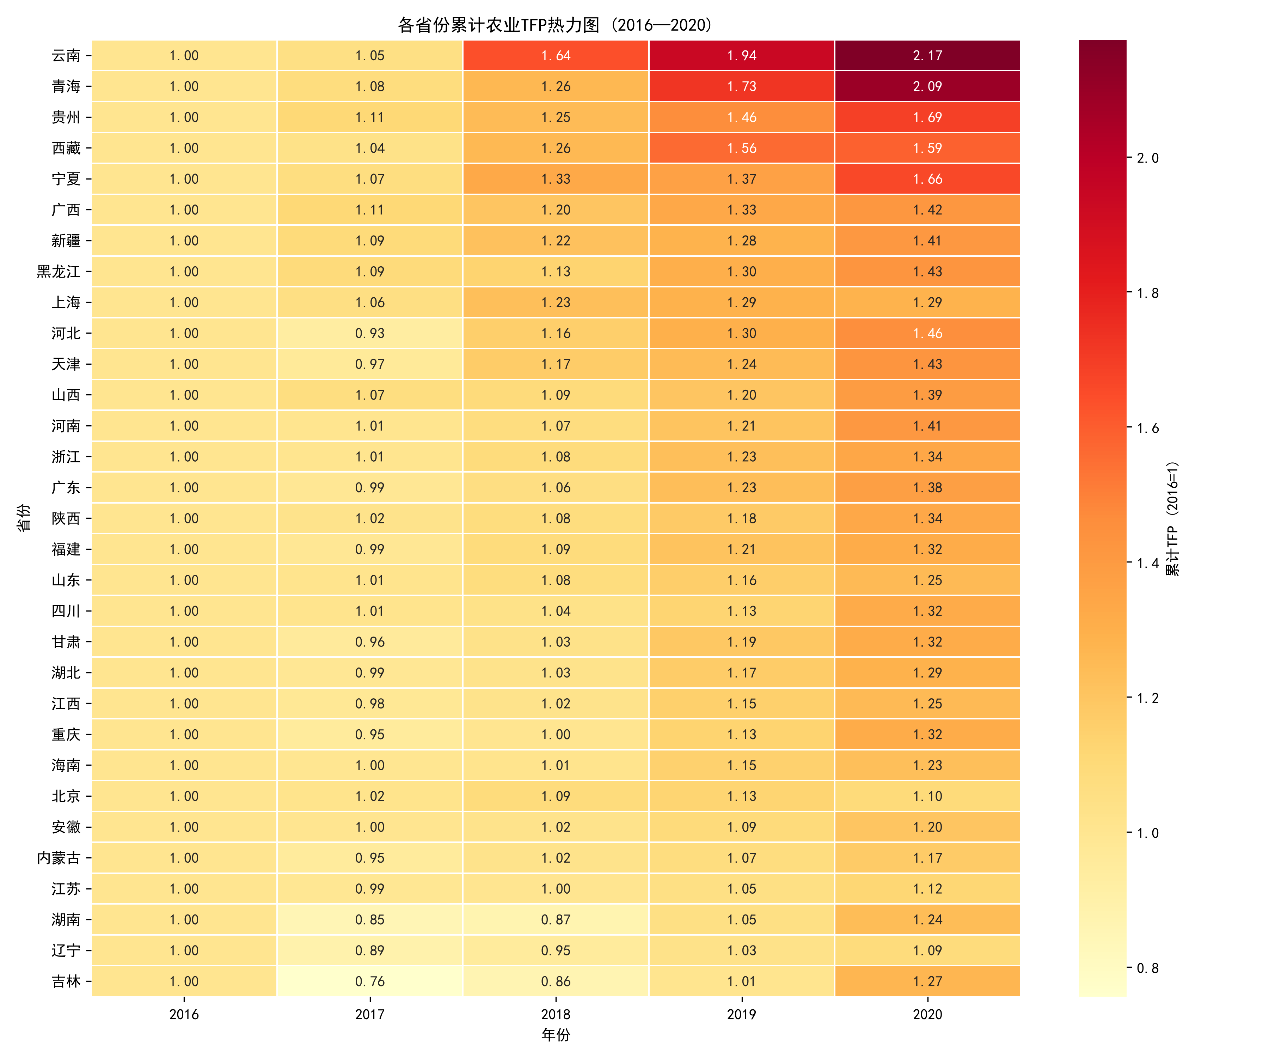
\includegraphics[width=5.76806in,height=4.80694in]{media/media/image3.png}

\emph{\textbf{Figure3：2016\textasciitilde2020年各省级行政区农业全要素生产率热力图}}

Figure3报告了各省2016---2020年累计农业全要数生产率（以2016为基期，基期值为1）。从全国视角上看，考察期内累计农业全要素生产率表现出稳步上升的趋势，至2020年全国多数省份都已超过了1.20，表明农业全要素生产率在样本期间实现了20\%及以上的累计增长。从省份差异来看，以2020年为例，云南（累计TFP为2.17）、青海（累计TFP为2.09）、贵州（累计TFP为1.69）等西部地区增速较为领先；而辽宁（累计TFP为1.09）、吉林（累计TFP为1.27）、江苏（累计TFP为1.12）等省份增速相对平缓

结合Figure1＆Figure2＆Figure3,TFP增长较为迅速的地区多为西部欠发达地区，而传统的农业大省或者是较为发达地区的增长速度反而趋于稳健，我们不难发现不同省级行政区划间的高质量发展指数与农业全要素生产率之间或许可能存在初步的线性相关关系。

\section{3描述性统计分析}\label{ux63cfux8ff0ux6027ux7edfux8ba1ux5206ux6790}

\subsection{3.1分布动态与区域差异}\label{ux5206ux5e03ux52a8ux6001ux4e0eux533aux57dfux5deeux5f02}

\subsubsection{3.1.1核密度估计}\label{ux6838ux5bc6ux5ea6ux4f30ux8ba1}

核密度估计是一种非线性估计方法，用于从已有的样本数据中估计总体的概率密度函数，本文引入该模型的目的是在还未做任何模型假设的前提下，直观的向我们展示经济高质量发展综合指数（Y）和农业全要素生产率（X）在样本期间的分布形态及其变化趋势

对于一组独立同分布的样本观测值\(x_{1},x_{2},\ldots,x_{n}\)，其核密度估计公式为：

\[\begin{array}{r}
\widehat{f_{h}}(x) = \frac{1}{nh}\sum_{i = 1}^{n}{K\left( \frac{x - x_{i}}{h} \right)}\qquad(14)
\end{array}\]

符号含义：

\(\widehat{f_{h}}(x)\)：核密度估计值，在点\(x\)处估计的密度值（即曲线高度）。

\(n\)样本量 参与估计的观测值个数（如 31 个省份）。

\(h\)带宽（Bandwidth） 控制估计精度的平滑参数。带宽越大，曲线越光滑（偏差增大，方差减小）；带宽越小，曲线越崎岖（偏差减小，方差增大）。

\(K(u)\)核函数（Kernel Function） 一个非负、对称、积分为1的权重函数，用于衡量样本点\(x_{i}\)对估计点\(x\)的贡献。

\(u\)标准化距离 表示估计点\(x\)与样本点\(x_{i}\)之间的标准化距离，即\(u = \frac{x - x_{i}}{h}\)。

值得注意的是\(K(u)\)核函数在实际应用中，通常选用高斯核即标准正态分布的密度函数：\(K(u) = \frac{1}{\sqrt{2\pi}}\exp\left( - \frac{u^{2}}{2} \right)\)

\emph{\textbf{Figure4核密度分析（全国视角）}}

\begin{longtable}[]{@{}
  >{\raggedright\arraybackslash}p{(\linewidth - 2\tabcolsep) * \real{0.5000}}
  >{\raggedright\arraybackslash}p{(\linewidth - 2\tabcolsep) * \real{0.5000}}@{}}
\toprule\noalign{}
\begin{minipage}[b]{\linewidth}\centering
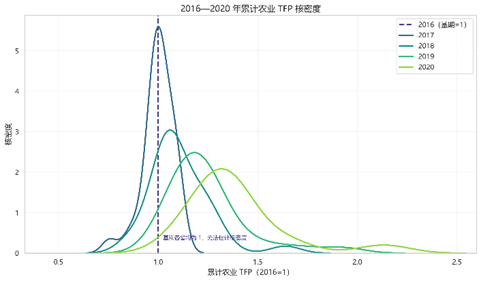
\includegraphics[width=3.20694in,height=1.87361in]{media/media/image4.png}
\end{minipage} & \begin{minipage}[b]{\linewidth}\centering
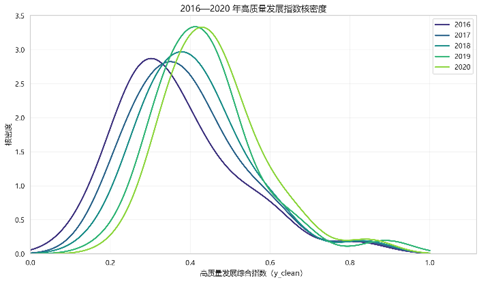
\includegraphics[width=3.20694in,height=1.87986in]{media/media/image5.png}
\end{minipage} \\
\midrule\noalign{}
\endhead
\bottomrule\noalign{}
\endlastfoot
\end{longtable}
Figure4分别展示了农业全要数生产率和经济高质量发展指数的核密度结果，第一张图：2016年是累计TFP的基期，各省均为1，因此不能形成对应的核密度曲线，只能用竖线表示，2017---2020年的曲线有明显的向右移动，全国累计TFP均值依次问1.001、1.109、1.245和1.386，说明农业全要素生产率总体呈现持续增长的态势，尤其是2018年以后增加的尤其明显。

但随着曲线的向右移动，其峰值总体下降、分布范围逐步扩大，标准差从2017年的0.076上升到2020年的0.245。意味着农业全要素生产率的增长并非是各省同步发生，不同省份的增长速度明显分化。

2028年以后曲线右侧出现越来越明显的长尾和局部次峰，2020年右尾延伸至2以上，这表明是存在少数省份的累计TFP增长是显著快于全国多数省份。

还应该注意的是，横轴是``累计TFP''，差异是具有逐年积累的性质，因此后期的宽分布是可以预期的而不是农业全要素生产率突然的分化。

第二张图则反映了在2016---2020年，全国高质量发展指数的核密度曲线持续向右移动，说明各省的高质量发展水平总体不断提高。全国均值由2016年的0.365提高至2020年的0.462累计提高约26.5\%.

而与此同时，标准差由0.149降为0.123，曲线整体逐渐收窄，说明在平均水平得到提升的同时，省际间的差距有所减少。但曲线右侧始终存在较长的拖尾，部分在累计农业TFP=0.8附近有轻微隆起。说明多数省份逐渐向中等水平集中，但头部地区仍明显领先。

\emph{\textbf{Figure5累计TFP}}\emph{\textbf{核密度分析（分区域、年份视角）}}

\begin{longtable}[]{@{}
  >{\centering\arraybackslash}p{(\linewidth - 2\tabcolsep) * \real{0.5000}}
  >{\centering\arraybackslash}p{(\linewidth - 2\tabcolsep) * \real{0.5000}}@{}}
\toprule\noalign{}
\begin{minipage}[b]{\linewidth}\centering
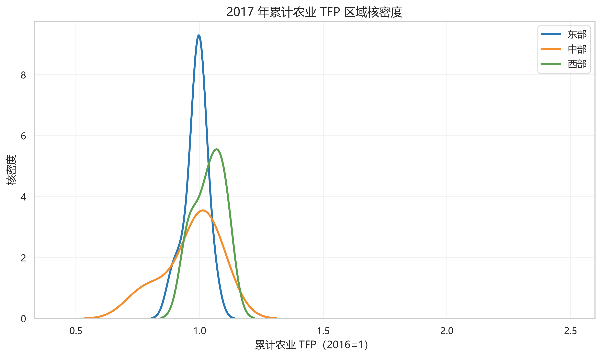
\includegraphics[width=2.73056in,height=1.62083in]{media/media/image6.png}
\end{minipage} & \begin{minipage}[b]{\linewidth}\centering
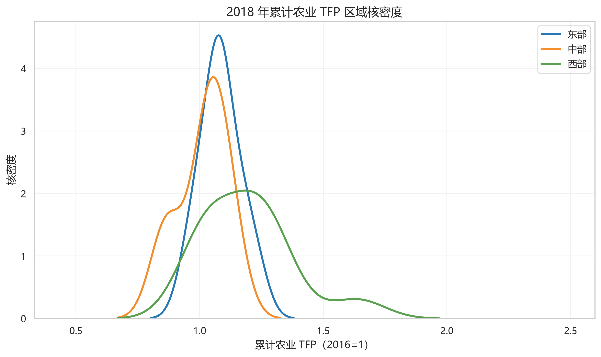
\includegraphics[width=2.73056in,height=1.62083in]{media/media/image7.png}
\end{minipage} \\
\midrule\noalign{}
\endhead
\bottomrule\noalign{}
\endlastfoot
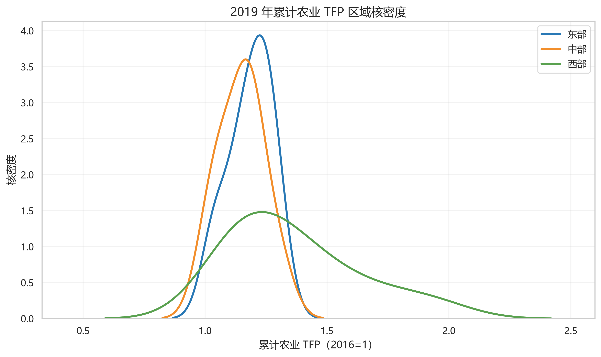
\includegraphics[width=2.73056in,height=1.62222in]{media/media/image8.png} & 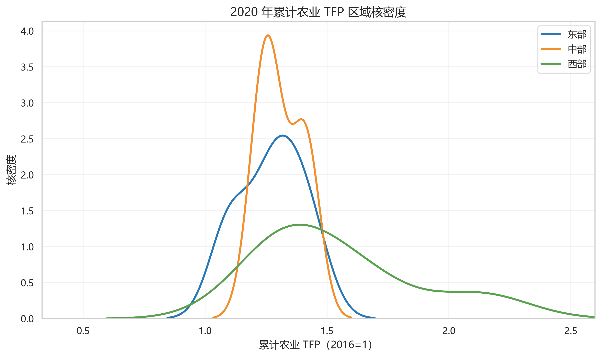
\includegraphics[width=2.73056in,height=1.62222in]{media/media/image9.png} \\
\end{longtable}
Figure5从不同时间段分东、中、西三部分区域对累计TFP进行了呈现，不难发现从2017到2020年，累计农业全要素生产率的核密度曲线大体呈现从高度集中到显著分化的变化轨迹。

2017年三大区域曲线高度重叠且呈现明显的尖峰状东部、中部、西部的累计均值分别为0.985、0.967和1.038因区域而造成的差异并不明显，东部曲线高度集中在1附近，标准差仅0.045，东部各省累计TFP变化幅度普遍较小，内部差异最小；西部曲线整体略位于东部右侧，均值高于1，西部地区在基期之后的第一年表现相对较好；中部曲线则明显更宽，且具有较长且明显的左拖尾，说明存在部分省份拉低了分布下端，表明2017年中部农业全要素生长率变化并不均等，且有部分省份出现了较明显的下降。

2018年，三条曲线开始从接近完全重合变得略有分离，其中东部、中部、西部的均值分别为1.084、1.013、1.194。东部地区微向右移动主要集中在TFP≈1.0-1.2附近，曲线较窄，总体上还属于温和增长且省际间差距相对有限；中部仍然具有一定的左侧肩部，吉林、湖南等省份累计TFP仍旧低于或接近于1，而多数中部省份处于1.0-1.1附近，显示中部内部存在一定的层次差异；西部地区有明显的向右移动且显著变宽，出现了右拖尾和出现右次峰的趋势，结合Figure3热力图以云南（累计TFP值为1.64）为代表的高数值省份明显高于其余西部省份，可以说西部的整体增长较快，但增长主要是由部分高增长省份带动，内部差异开始显现并扩大

2019年，东部、中部和西部均值分别为1.185、1.148和1.364。东部和中部曲线比较靠近，二者主体都集中在1.1---1.3附近，两省份的累计TFP水平比较接近。东部略微偏右，但均值差距很小。与之不同，西部曲线明显更宽、更平、并伴有显著的右拖尾。云南达到约1.94、青海约1.73，西藏约1.56，明显高于西部主体省份，``整体提高与少数省份拉动''的特征依旧不变

到了2020年，东部、中部和西部累计TFP均值分别为1.272、1.311和1.542。东部曲线主要集中在1.2---1.4附近，分布相对平缓。北京、辽宁、江苏处于较低端，而天津、河北等省份则相对比较高，可以说东部地区的内部差异较前期有所扩大；中部曲线的标准差仅0.086，多数省份位于1.2---1.4之间，呈现较为稳定、均衡的增长状态。不可忽略的是右侧的轻微肩部，轻微肩部的存在反映出中部地区的内部仍存在少量层次差异，但总体并不强烈；西部曲线最宽，并有清晰的右托拖尾，主体省份集中在1.3---1.7附近，西部标准差达到0.316，远高于东部的0.129和中部的0.086。但也可能是因为受到低基期、投入收缩、DEA前沿变化以及累计指数放大效应的影响，我们不能简单等同于西部农业综合发展水平已经超过东部。

\emph{\textbf{Figure6经济高质量发展综合指数核密度分析（分区域、年份视角）}}

\begin{longtable}[]{@{}
  >{\raggedright\arraybackslash}p{(\linewidth - 4\tabcolsep) * \real{0.3334}}
  >{\raggedright\arraybackslash}p{(\linewidth - 4\tabcolsep) * \real{0.3333}}
  >{\raggedright\arraybackslash}p{(\linewidth - 4\tabcolsep) * \real{0.3333}}@{}}
\toprule\noalign{}
\begin{minipage}[b]{\linewidth}\raggedright
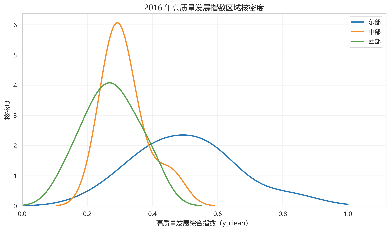
\includegraphics[width=1.77083in,height=1.05139in]{media/media/image10.png}
\end{minipage} & \begin{minipage}[b]{\linewidth}\raggedright
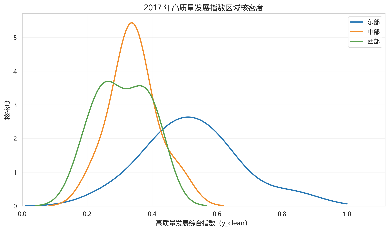
\includegraphics[width=1.77014in,height=1.05069in]{media/media/image11.png}
\end{minipage} & \begin{minipage}[b]{\linewidth}\raggedright
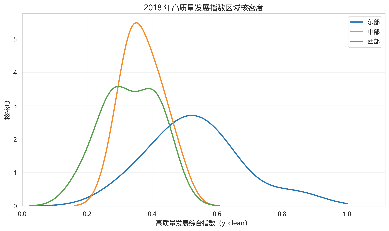
\includegraphics[width=1.77014in,height=1.05069in]{media/media/image12.png}
\end{minipage} \\
\midrule\noalign{}
\endhead
\bottomrule\noalign{}
\endlastfoot
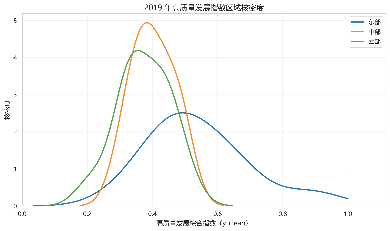
\includegraphics[width=1.77083in,height=1.05139in]{media/media/image13.png} & 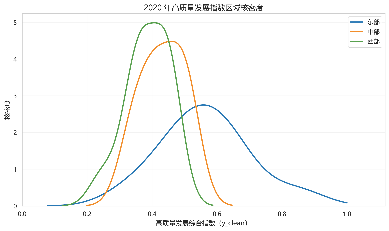
\includegraphics[width=1.77014in,height=1.05069in]{media/media/image14.png} & \\
\end{longtable}
Figure6呈现了2016-2020分地区的高质量发展综合指数的核密度分析

2016---2020年，东、中、西部地区高质量发展指数的核密度曲线呈现不同程度的右移，表明在样本存续期内三大区域的高质量发展综合指数的总体水平持续提高。从相对位置来看，东部始终位于中、西部右侧，中部总体位于西部右侧，区域分布长期呈现``东部领先、中部次之、西部相对滞后''的梯度格局。区域均值也印证了这一特征：东部均值自2016年的0.502提高为2020年的0.565，中部从0.316提升至0.432，西部地区由0.272提高为0.387.

而从区域差异上来看，东部核密度曲线整体较为宽缓，并始终存在明显的拖尾，证明东部地区虽然总体经济高质量发展水平最高，但内部的差异也比较突出：北京、上海、江苏等省份处于较高水平，而河北、海南等省份相对偏低，表现出比较明显的区域内部层次。相比之下中部曲线峰值较高分布也相对集中，可以说明中部多数省份的高质量发展水平较为接近，内部差异不明显或较小。西部曲线在部分年份呈现平台化或若双峰特征，是证明西部地区可能存在一定发展梯度的证据。但介于区域样本数据有限，我们更宜将其解释为初步分化迹象。

若从动态变化出发，中西部核密度的右移速度相对较快，与东部的距离有所缩小：1.东部与西部的均值差距由2016年的约0.229下降至2020年的约0.178，东部与中部的均值差距也自约0.186下降为0.132。

与此同时，中部与西部曲线的重叠程度逐渐提高，这能说明两地区有越来越多的省份进入相近的发展区间。

总体而言，在样本期间我国的省际高质量发展既保持了东部领先的基本空间格局，也出现了中西部加快追赶和区域差距逐步收敛的态势。

\subsubsection{3.1.2Dagum基尼系数}\label{dagumux57faux5c3cux7cfbux6570}

核密度估计能够刻画分布位置、峰态及拖尾变化，但无法定量识别差异究竟来自区域内部、区域之间，还是不同区域分布交叉。为此，本文采用Dagum（1997）基尼系数及其子群分解方法，将省际总体差异分解为区域内差异、区域间净差异和超变密度三部分。相较于传统基尼分解，该方法能够处理不同区域分布相互重叠的问题。

\[G=\frac{\sum_j\sum_h\sum_i\sum_r\lvert x_{ji}-x_{hr}\rvert}{2n^2\bar{x}}\]

式中，\(x_{ji}\)表示区域j中第i个省份的指标值，n为省份总数，\(\bar{x}\)为全国均值。设\(p_j=n_j/n\)为区域省份数量份额，\(s_j=n_j\bar{x}_j/(n\bar{x})\)为区域指标份额，\(G_{jj}\)和\(G_{jh}\)分别表示区域内部及区域之间的基尼系数，则总体基尼系数可分解为：

\[G=G_w+G_{nb}+G_t\]

\[G_w=\sum_j G_{jj}p_js_j\]

\[G_{nb}=\sum_{j>h}G_{jh}D_{jh}(p_js_h+p_hs_j)\]

\[G_t=\sum_{j>h}G_{jh}(1-D_{jh})(p_js_h+p_hs_j)\]

其中，Gw为区域内差异，Gnb为区域间净差异，Gt为超变密度；\(D_{jh}=(d_{jh}-p_{jh})/(d_{jh}+p_{jh})\)为区域间相对影响系数。\(d_{jh}\)表示高均值区域样本超过低均值区域样本的平均超距，\(p_{jh}\)表示低均值区域样本反超高均值区域样本产生的平均交叉差异。Dⱼₕ越接近1，说明两区域分布分离越明显；越接近0，说明分布重叠越充分。

\begin{longtable}[]{@{}
  >{\centering\arraybackslash}p{(\linewidth - 10\tabcolsep) * \real{0.1831}}
  >{\centering\arraybackslash}p{(\linewidth - 10\tabcolsep) * \real{0.0959}}
  >{\centering\arraybackslash}p{(\linewidth - 10\tabcolsep) * \real{0.1308}}
  >{\centering\arraybackslash}p{(\linewidth - 10\tabcolsep) * \real{0.1483}}
  >{\centering\arraybackslash}p{(\linewidth - 10\tabcolsep) * \real{0.2180}}
  >{\centering\arraybackslash}p{(\linewidth - 10\tabcolsep) * \real{0.1744}}@{}}
\caption{表3 Dagum基尼系数及差异来源贡献率}\tabularnewline
\toprule\noalign{}
\begin{minipage}[b]{\linewidth}\centering
\textbf{变量}
\end{minipage} & \begin{minipage}[b]{\linewidth}\centering
\textbf{年份}
\end{minipage} & \begin{minipage}[b]{\linewidth}\centering
\textbf{总基尼}
\end{minipage} & \begin{minipage}[b]{\linewidth}\centering
\textbf{区域内}
\end{minipage} & \begin{minipage}[b]{\linewidth}\centering
\textbf{区域间净差异}
\end{minipage} & \begin{minipage}[b]{\linewidth}\centering
\textbf{超变密度}
\end{minipage} \\
\midrule\noalign{}
\endfirsthead
\toprule\noalign{}
\begin{minipage}[b]{\linewidth}\centering
\textbf{变量}
\end{minipage} & \begin{minipage}[b]{\linewidth}\centering
\textbf{年份}
\end{minipage} & \begin{minipage}[b]{\linewidth}\centering
\textbf{总基尼}
\end{minipage} & \begin{minipage}[b]{\linewidth}\centering
\textbf{区域内}
\end{minipage} & \begin{minipage}[b]{\linewidth}\centering
\textbf{区域间净差异}
\end{minipage} & \begin{minipage}[b]{\linewidth}\centering
\textbf{超变密度}
\end{minipage} \\
\midrule\noalign{}
\endhead
\bottomrule\noalign{}
\endlastfoot
高质量发展 & 2016 & 0.2151 & 23.96\% & 67.30\% & 8.73\% \\
高质量发展 & 2017 & 0.1924 & 24.21\% & 64.97\% & 10.82\% \\
高质量发展 & 2018 & 0.1742 & 25.31\% & 63.96\% & 10.73\% \\
高质量发展 & 2019 & 0.1516 & 27.86\% & 57.95\% & 14.18\% \\
高质量发展 & 2020 & 0.1414 & 25.57\% & 62.87\% & 11.56\% \\
累计TFP & 2016 & 0.0000 & --- & --- & --- \\
累计TFP & 2017 & 0.0397 & 28.58\% & 40.20\% & 31.22\% \\
累计TFP & 2018 & 0.0675 & 29.64\% & 53.04\% & 17.32\% \\
累计TFP & 2019 & 0.0777 & 30.83\% & 51.33\% & 17.84\% \\
累计TFP & 2020 & 0.0846 & 30.48\% & 54.28\% & 15.24\% \\
\end{longtable}

注：三类贡献率之和为100\%；累计TFP在2016年为共同基期，故该年贡献率不计算。

结果显示，高质量发展指数的总体基尼系数由2016年的0.2151持续下降至2020年的0.1414，累计降幅约34.3\%，表明省际高质量发展差异呈稳定收敛。区域间净差异的贡献率始终位于57.95\%---67.30\%，是总体差异的首要来源；区域内差异约占24\%---28\%，超变密度约占9\%---14\%。因此，现阶段高质量发展不平衡主要体现为东中西部整体发展梯度，而不是单一区域内部的离散。

累计TFP在2016年被统一设为1，故该年差异为0，不具有横截面比较含义。2017---2020年其总基尼由0.0397上升至0.0846，表明累计增长路径逐步分化。区域间净差异贡献率由40.20\%升至54.28\%，超变密度由31.22\%降至15.24\%，说明区域主体分布逐渐拉开。区域内结果进一步表明，西部TFP区域内基尼由0.0309上升至0.1036，是总体分化扩大的重要来源。需要强调的是，Dagum分解揭示的是差异的空间统计构成，而非差异形成的因果机制。




\begin{figure}[htbp]
\centering
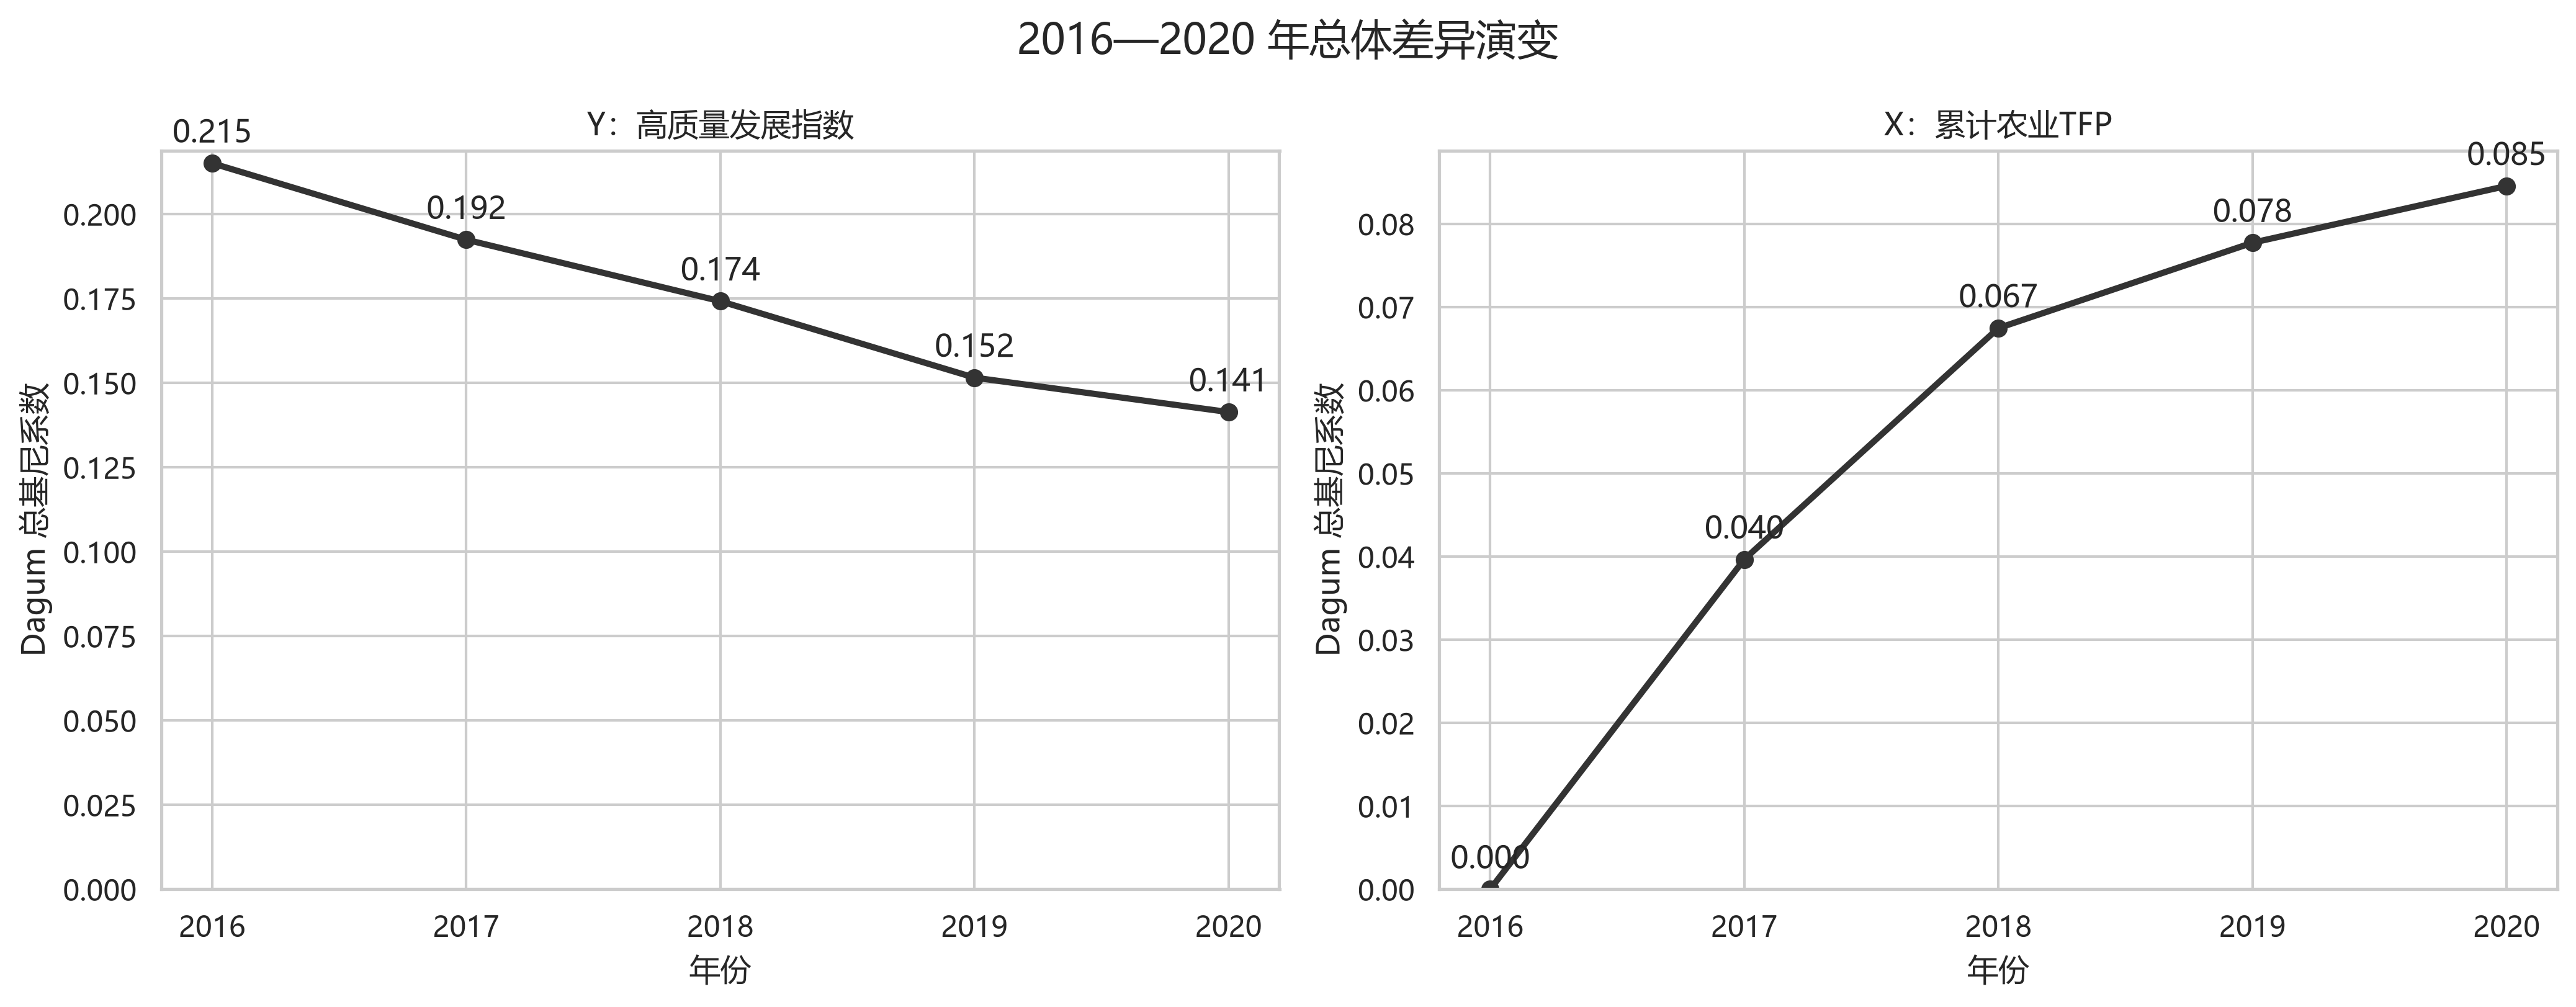
\includegraphics[width=\linewidth,height=0.82\textheight,keepaspectratio]{media/media/image15.png}
\caption*{Figure7 高质量发展指数与累计农业TFP的Dagum总基尼系数}
\end{figure}
\begin{figure}[htbp]
\centering
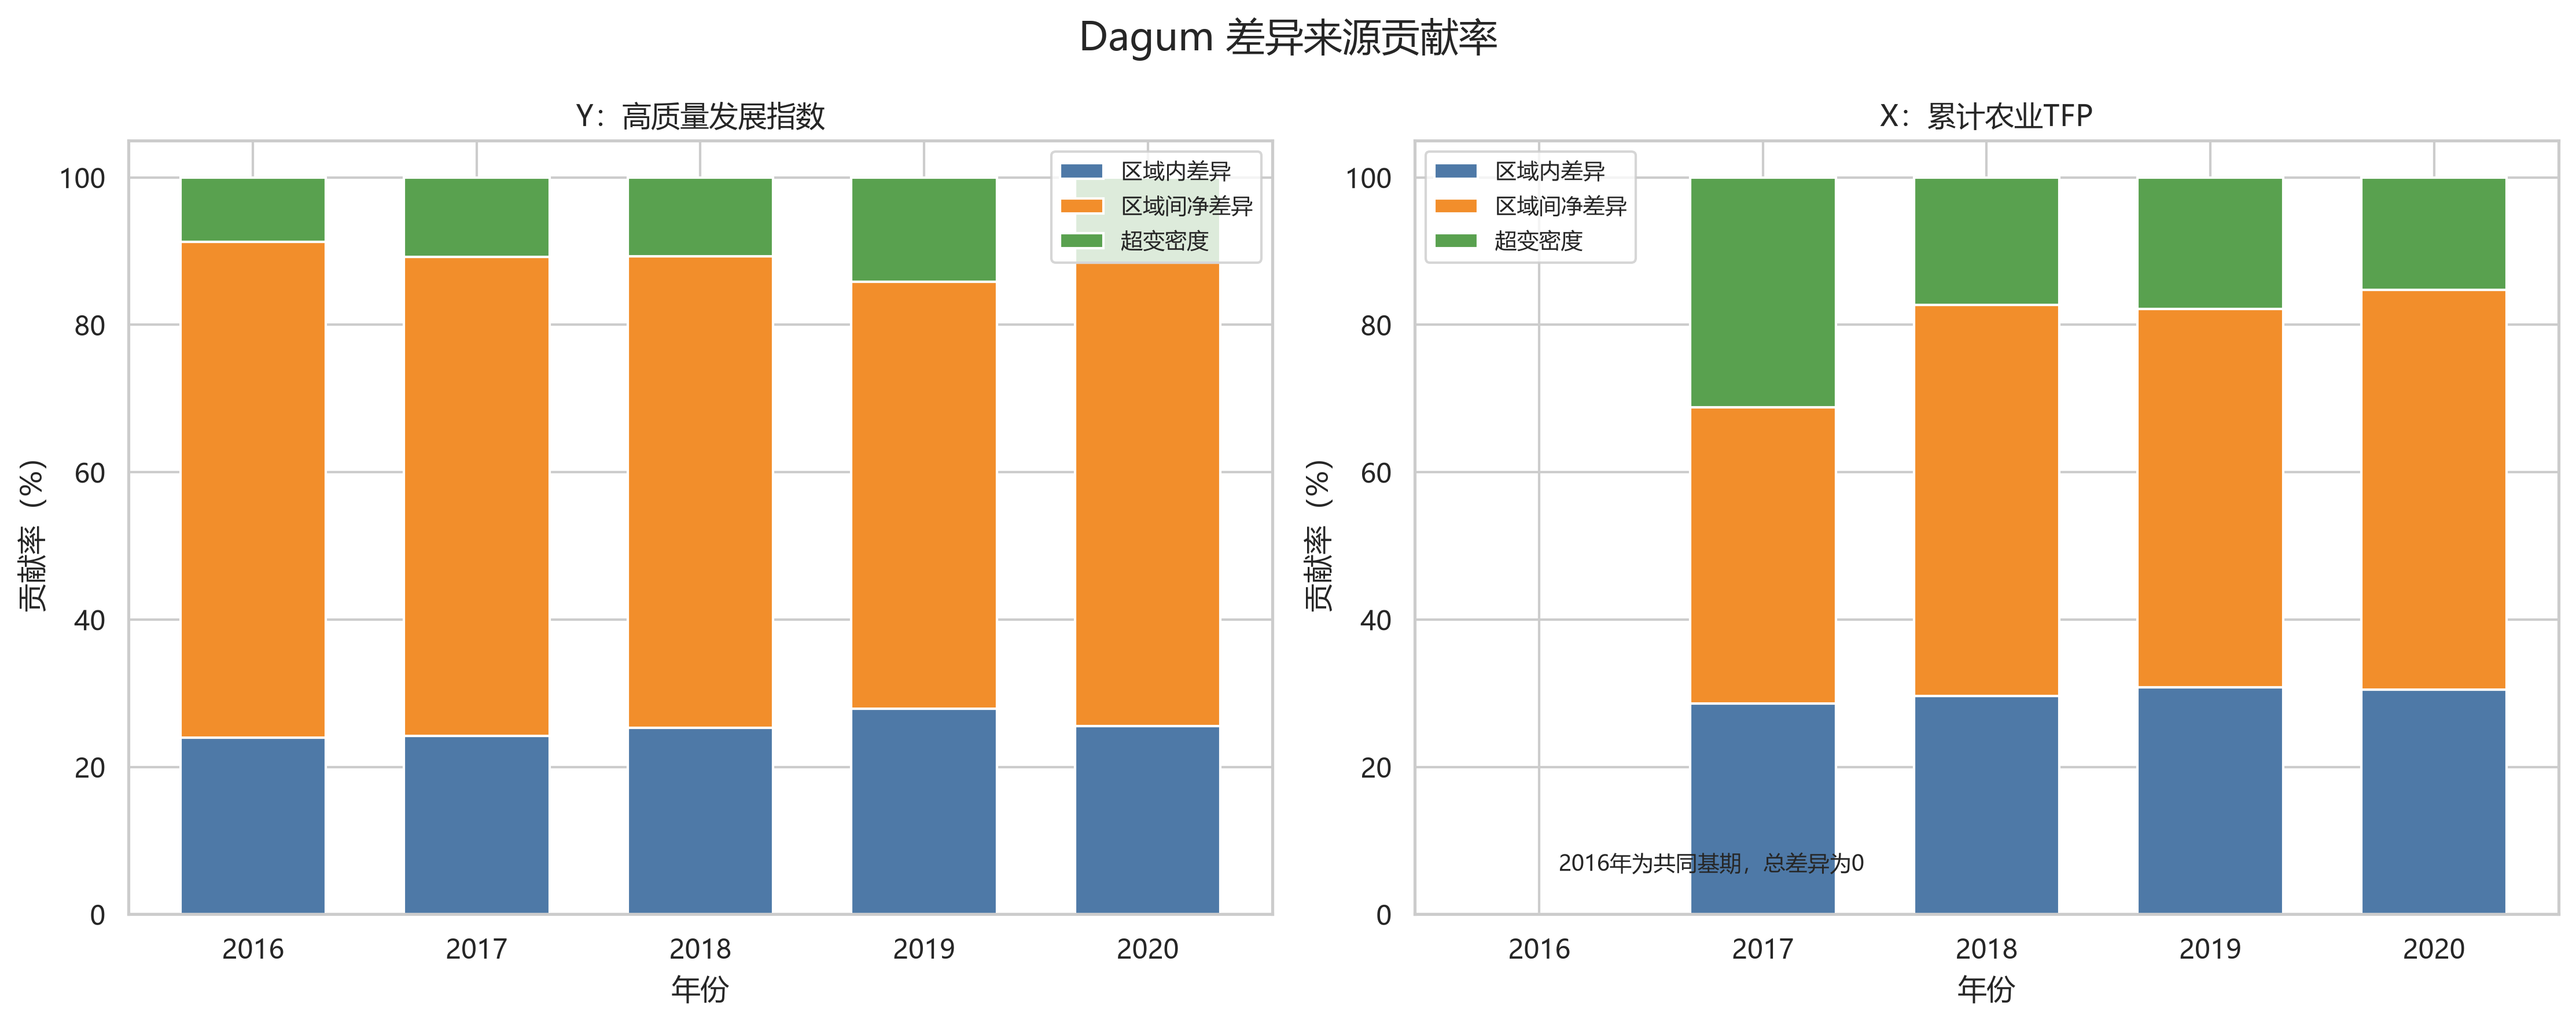
\includegraphics[width=\linewidth,height=0.82\textheight,keepaspectratio]{media/media/image16.png}
\caption*{Figure8 Dagum基尼系数差异来源贡献率}
\end{figure}


\subsection{3.3空间自相关初步检验}\label{ux7a7aux95f4ux81eaux76f8ux5173ux521dux6b65ux68c0ux9a8c}

\subsubsection{3.3.1全局莫兰指数}\label{ux5168ux5c40ux83abux5170ux6307ux6570}

为检验高质量发展及农业TFP是否具有空间依赖性，本文以省级行政区接壤关系构建二元邻接矩阵，并进行行标准化。海南不存在陆地邻省，为避免空间孤岛，将其与地理距离最近且联系密切的广东桥接。全局Moran指数定义为：

\[I=\frac{n}{S_0}\frac{\sum_i\sum_jw_{ij}(x_i-\bar{x})(x_j-\bar{x})}{\sum_i(x_i-\bar{x})^2}\]

其中，\(w_{ij}\)为空间权重，\(S_0=\sum_i\sum_jw_{ij}\)。I大于其随机期望值－1/(n－1)表示正空间相关，小于期望值表示负空间相关。显著性采用999次随机置换获得伪p值。

\begin{longtable}[]{@{}
  >{\centering\arraybackslash}p{(\linewidth - 8\tabcolsep) * \real{0.2265}}
  >{\centering\arraybackslash}p{(\linewidth - 8\tabcolsep) * \real{0.1132}}
  >{\centering\arraybackslash}p{(\linewidth - 8\tabcolsep) * \real{0.1829}}
  >{\centering\arraybackslash}p{(\linewidth - 8\tabcolsep) * \real{0.1742}}
  >{\centering\arraybackslash}p{(\linewidth - 8\tabcolsep) * \real{0.1742}}@{}}
\caption{表4 全局Moran指数及置换检验}\tabularnewline
\toprule\noalign{}
\begin{minipage}[b]{\linewidth}\centering
\textbf{变量}
\end{minipage} & \begin{minipage}[b]{\linewidth}\centering
\textbf{年份}
\end{minipage} & \begin{minipage}[b]{\linewidth}\centering
\textbf{Moran\textquotesingle s I}
\end{minipage} & \begin{minipage}[b]{\linewidth}\centering
\textbf{置换z值}
\end{minipage} & \begin{minipage}[b]{\linewidth}\centering
\textbf{置换p值}
\end{minipage} \\
\midrule\noalign{}
\endfirsthead
\toprule\noalign{}
\begin{minipage}[b]{\linewidth}\centering
\textbf{变量}
\end{minipage} & \begin{minipage}[b]{\linewidth}\centering
\textbf{年份}
\end{minipage} & \begin{minipage}[b]{\linewidth}\centering
\textbf{Moran\textquotesingle s I}
\end{minipage} & \begin{minipage}[b]{\linewidth}\centering
\textbf{置换z值}
\end{minipage} & \begin{minipage}[b]{\linewidth}\centering
\textbf{置换p值}
\end{minipage} \\
\midrule\noalign{}
\endhead
\bottomrule\noalign{}
\endlastfoot
高质量发展 & 2016 & 0.402 & 3.959 & 0.001 \\
高质量发展 & 2017 & 0.378 & 3.711 & 0.001 \\
高质量发展 & 2018 & 0.365 & 3.461 & 0.003 \\
高质量发展 & 2019 & 0.236 & 2.346 & 0.019 \\
高质量发展 & 2020 & 0.356 & 3.436 & 0.004 \\
累计TFP & 2016 & --- & --- & 共同基期 \\
累计TFP & 2017 & 0.069 & 0.900 & 0.189 \\
累计TFP & 2018 & 0.201 & 2.155 & 0.030 \\
累计TFP & 2019 & 0.249 & 2.440 & 0.020 \\
累计TFP & 2020 & 0.168 & 1.931 & 0.041 \\
\end{longtable}

注：伪p值基于999次随机置换；累计TFP在2016年为共同基期，横截面无差异。

高质量发展指数的Moran值在0.236---0.402之间，所有年份均在5\%水平显著为正，说明相近省份之间长期存在高---高或低---低集聚。2019年空间相关程度有所减弱，但2020年重新升至0.356。累计TFP在2017年的Moran值为0.069且不显著，表明基期后初始增长主要体现为省份个体波动；2018---2020年Moran值分别为0.201、0.249和0.168，均通过5\%置换检验，说明TFP增长逐步形成空间集聚，但2020年集聚强度有所回落。




\begin{figure}[htbp]
\centering
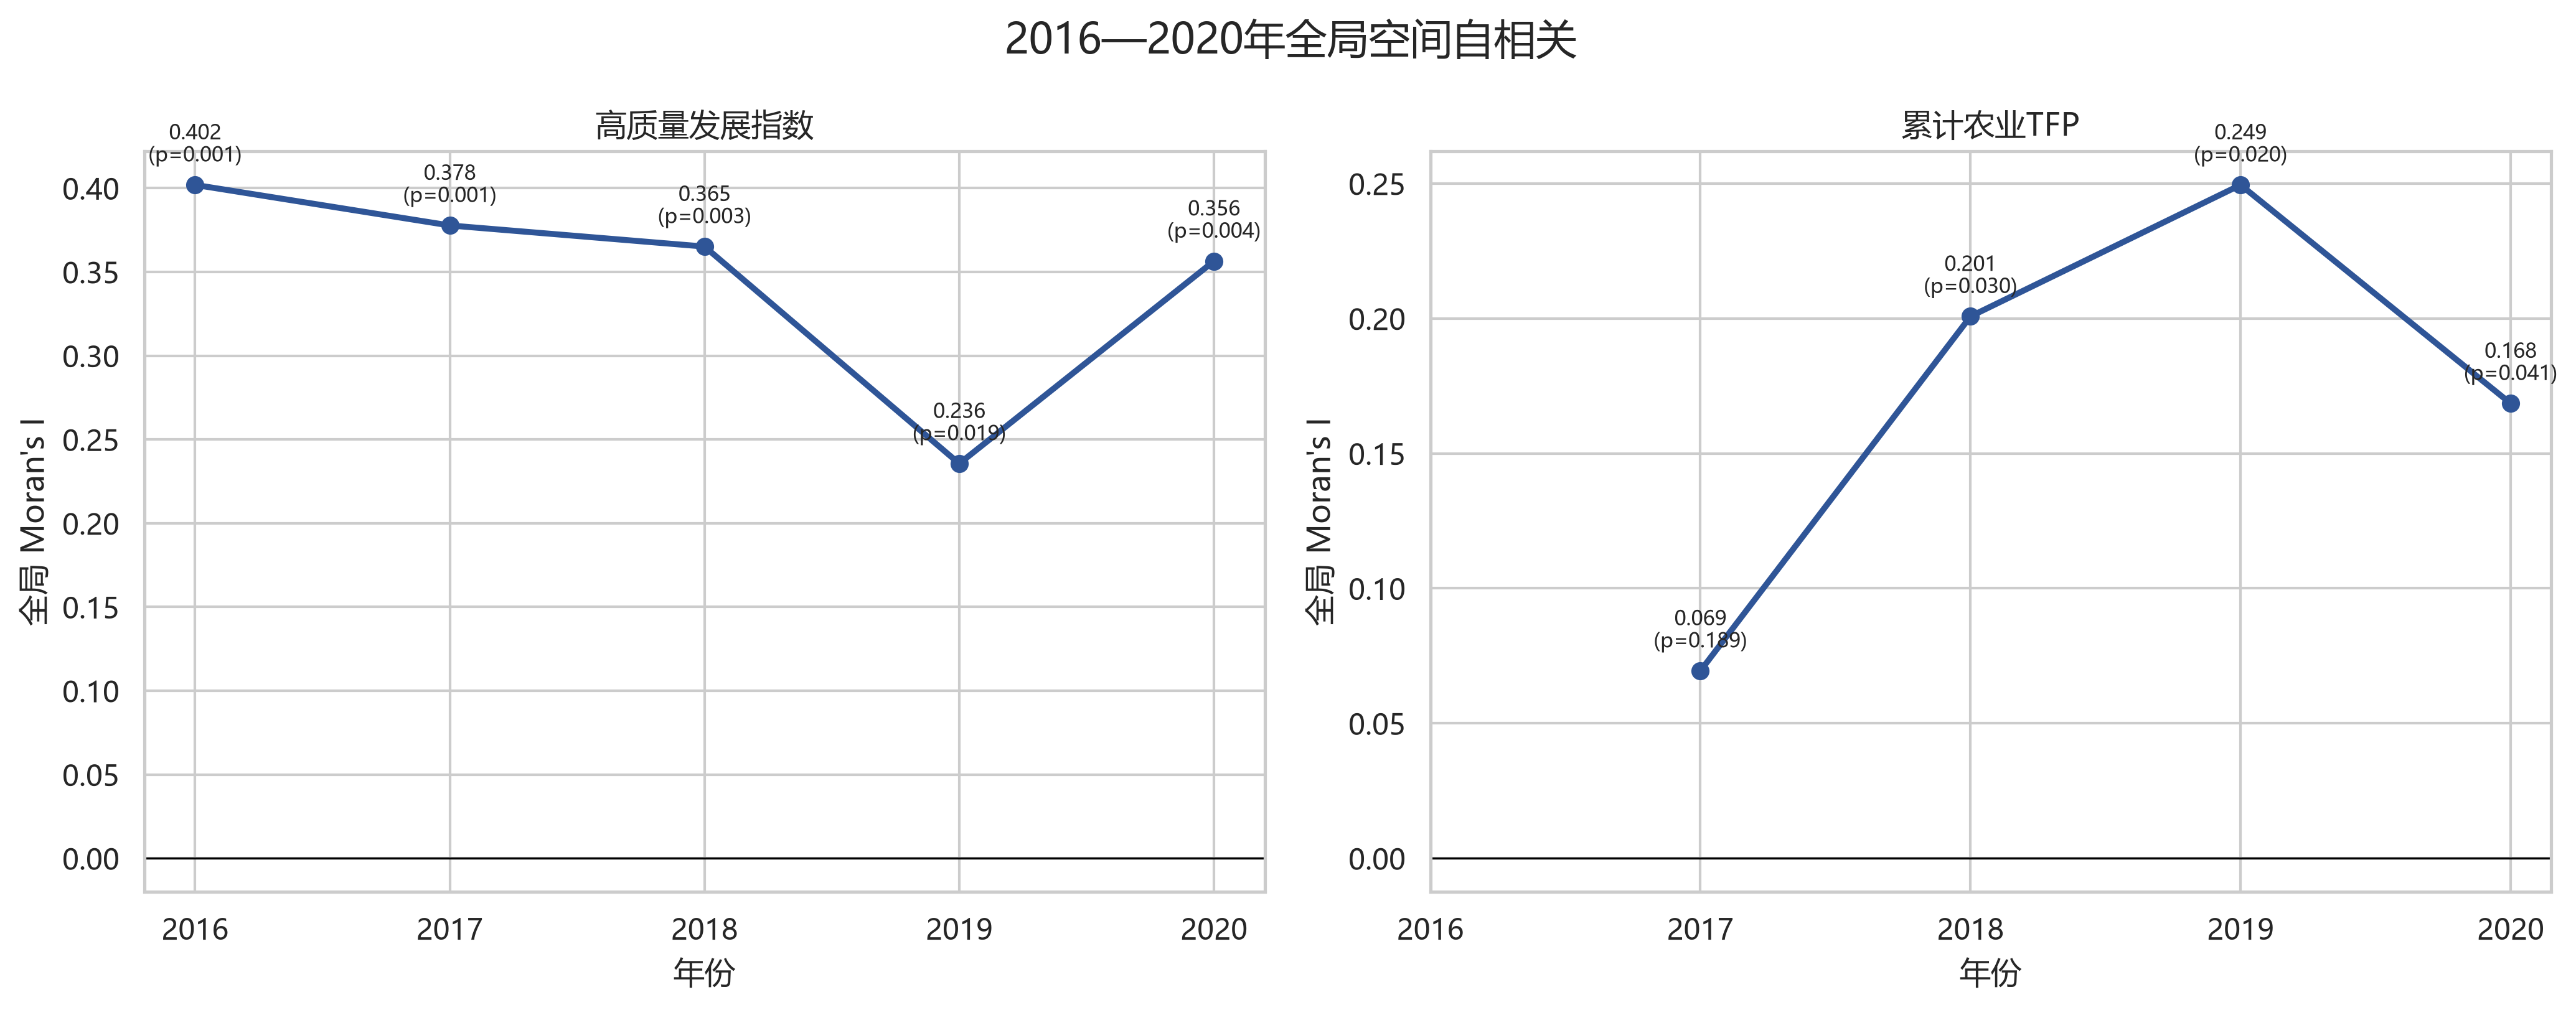
\includegraphics[width=\linewidth,height=0.82\textheight,keepaspectratio]{media/media/image17.png}
\caption*{Figure9 高质量发展指数与累计农业TFP的全局Moran指数}
\end{figure}
\begin{figure}[htbp]
\centering
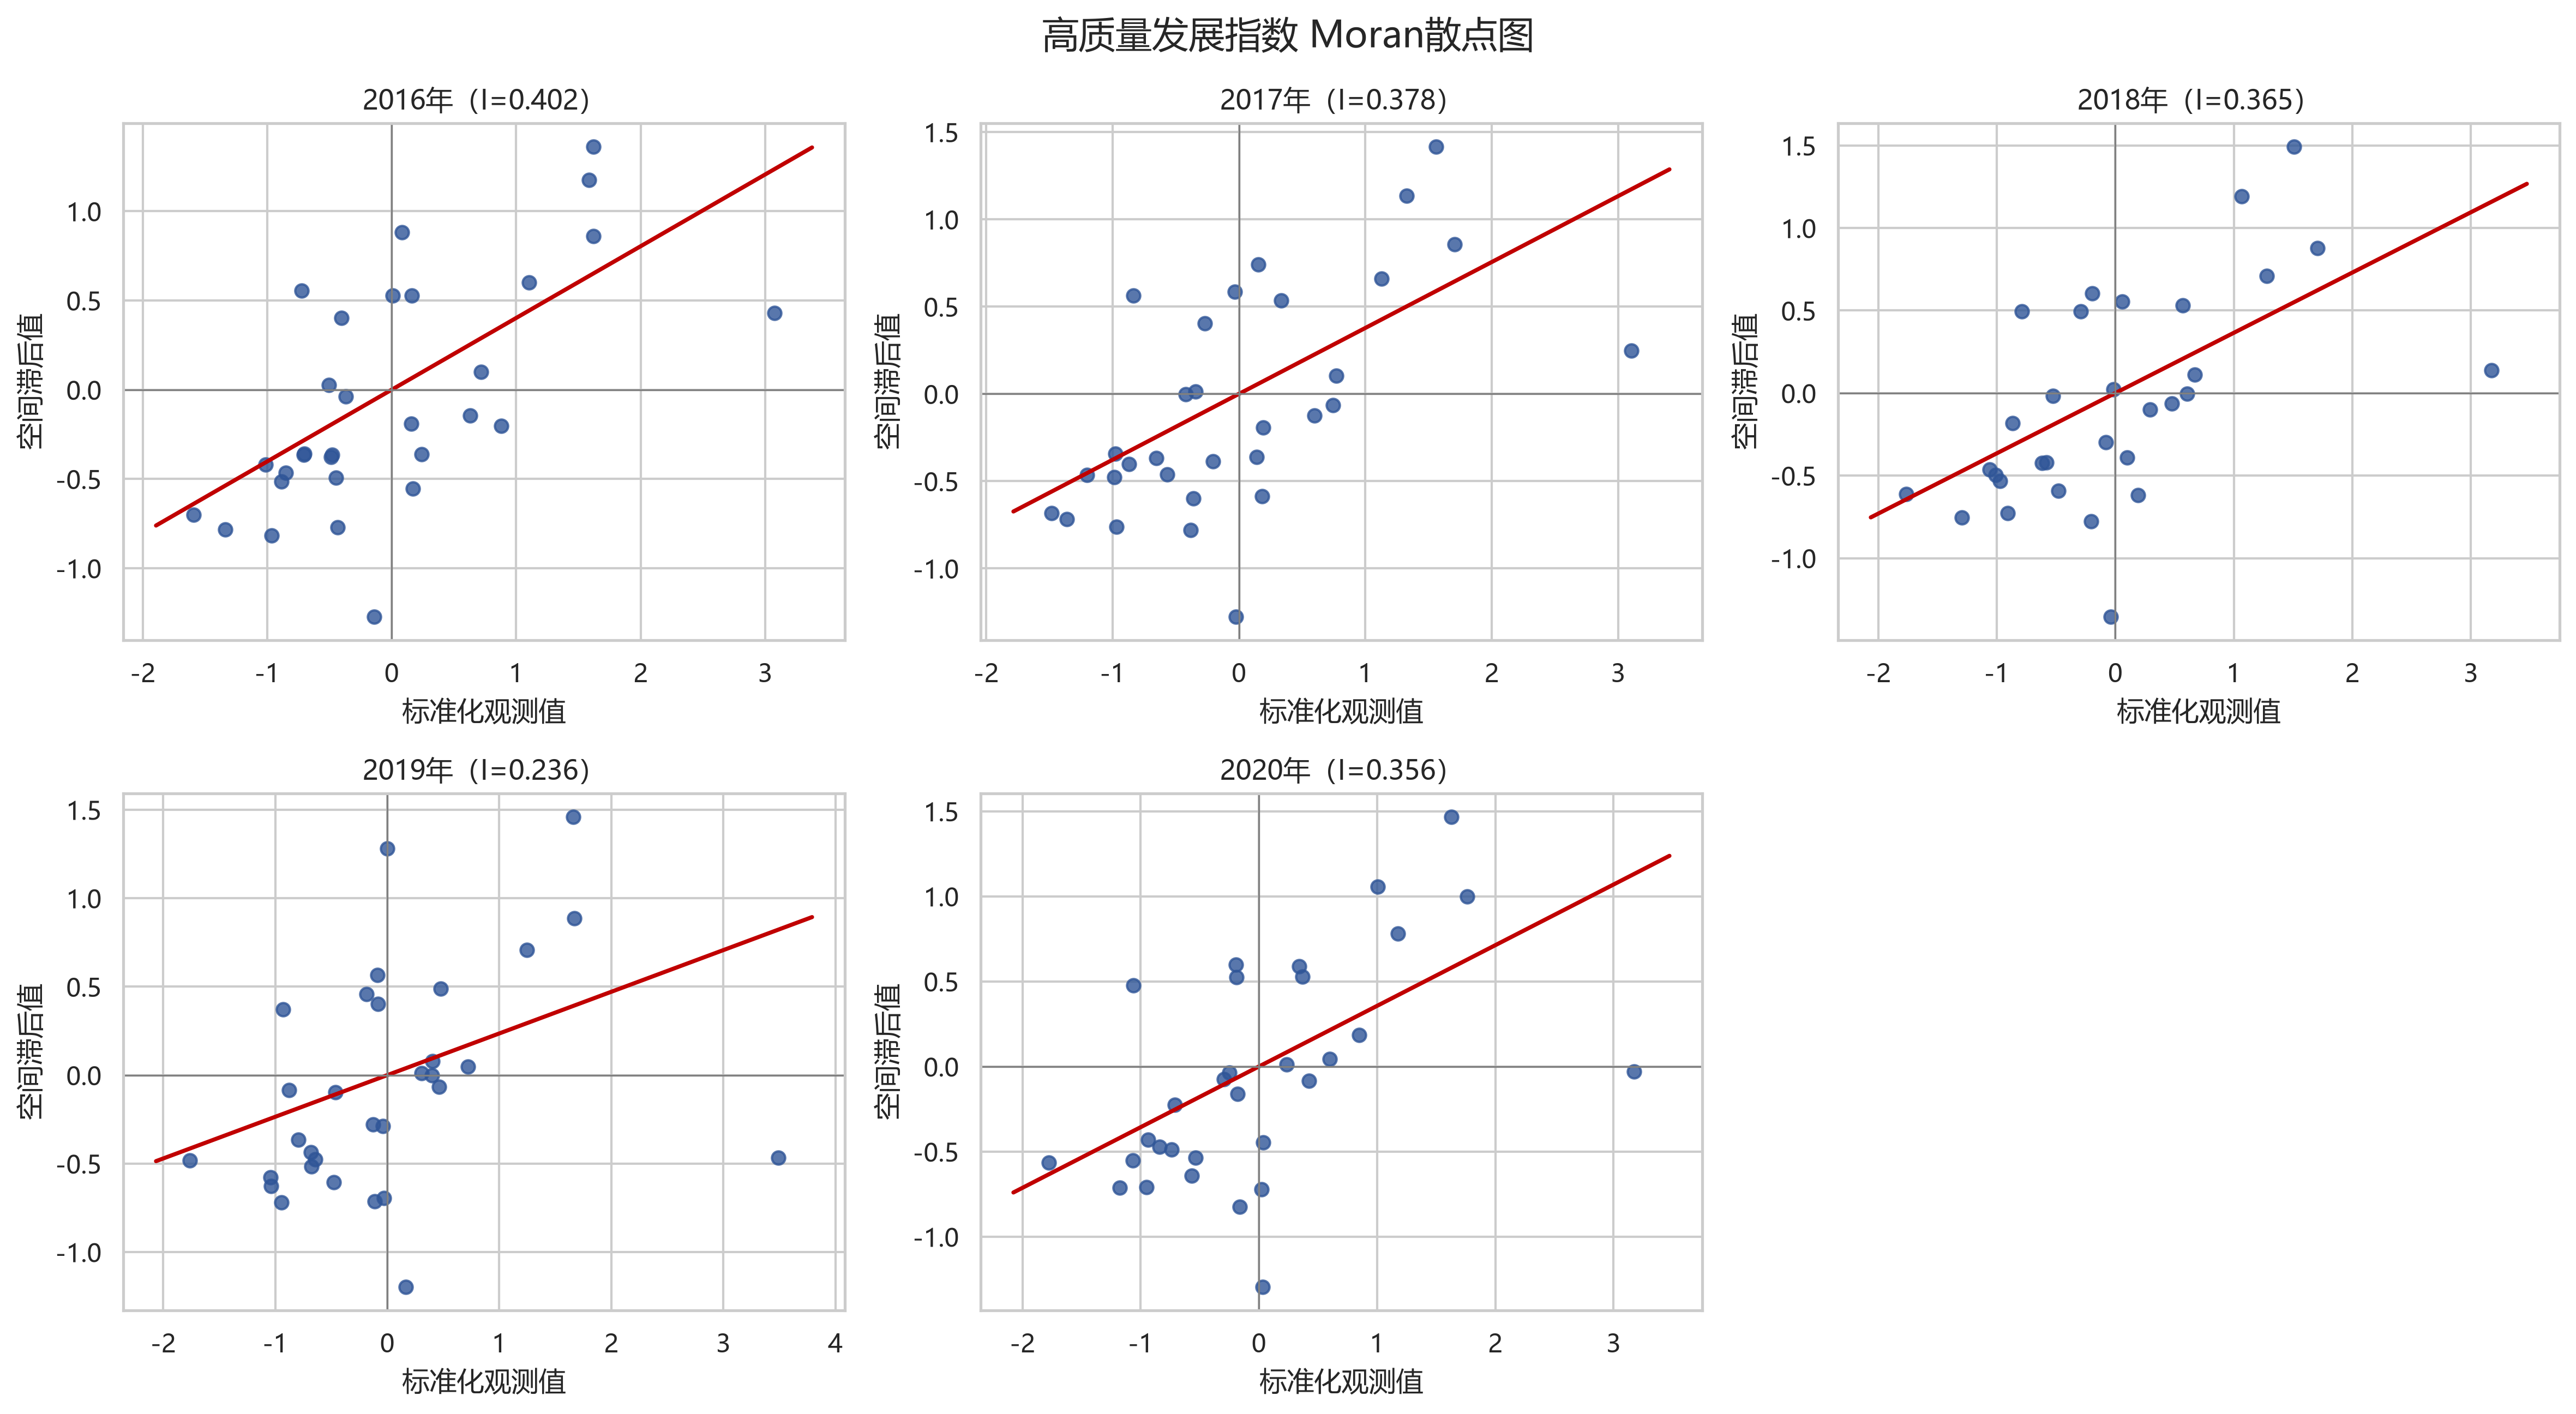
\includegraphics[width=\linewidth,height=0.82\textheight,keepaspectratio]{media/media/image18.png}
\caption*{Figure10 高质量发展指数Moran散点图}
\end{figure}


\subsubsection{3.3.2局部莫兰指数}\label{ux5c40ux90e8ux83abux5170ux6307ux6570}

全局指标仅反映总体空间相关，无法识别具体集聚位置，因而进一步采用Anselin局部Moran指数（LISA）：

\[I_i=z_i\sum_jw_{ij}z_j\]

其中，\(z_i\)为标准化指标值。依据自身取值与空间滞后值的符号，将省份划分为高---高（HH）、低---低（LL）、高---低（HL）和低---高（LH）四类；仅将999次置换检验p\textless0.05的结果认定为显著局部集聚。

高质量发展指数的局部集聚格局具有较强稳定性。以2020年为例，上海、江苏和浙江表现为显著HH集聚，内蒙古、四川、云南和青海表现为显著LL集聚，新疆表现为HL型空间离群。该结果表明长三角形成了连续高值集聚，而部分西部省份仍处于低值邻接环境。累计TFP的局部格局波动更大，2020年广西、西藏和新疆为HH，浙江为LL，河北为HL，四川为LH。由于局部检验数量较多且样本期较短，这些结果应主要作为空间模型设定的诊断依据，不宜作强因果解释。




\begin{figure}[htbp]
\centering
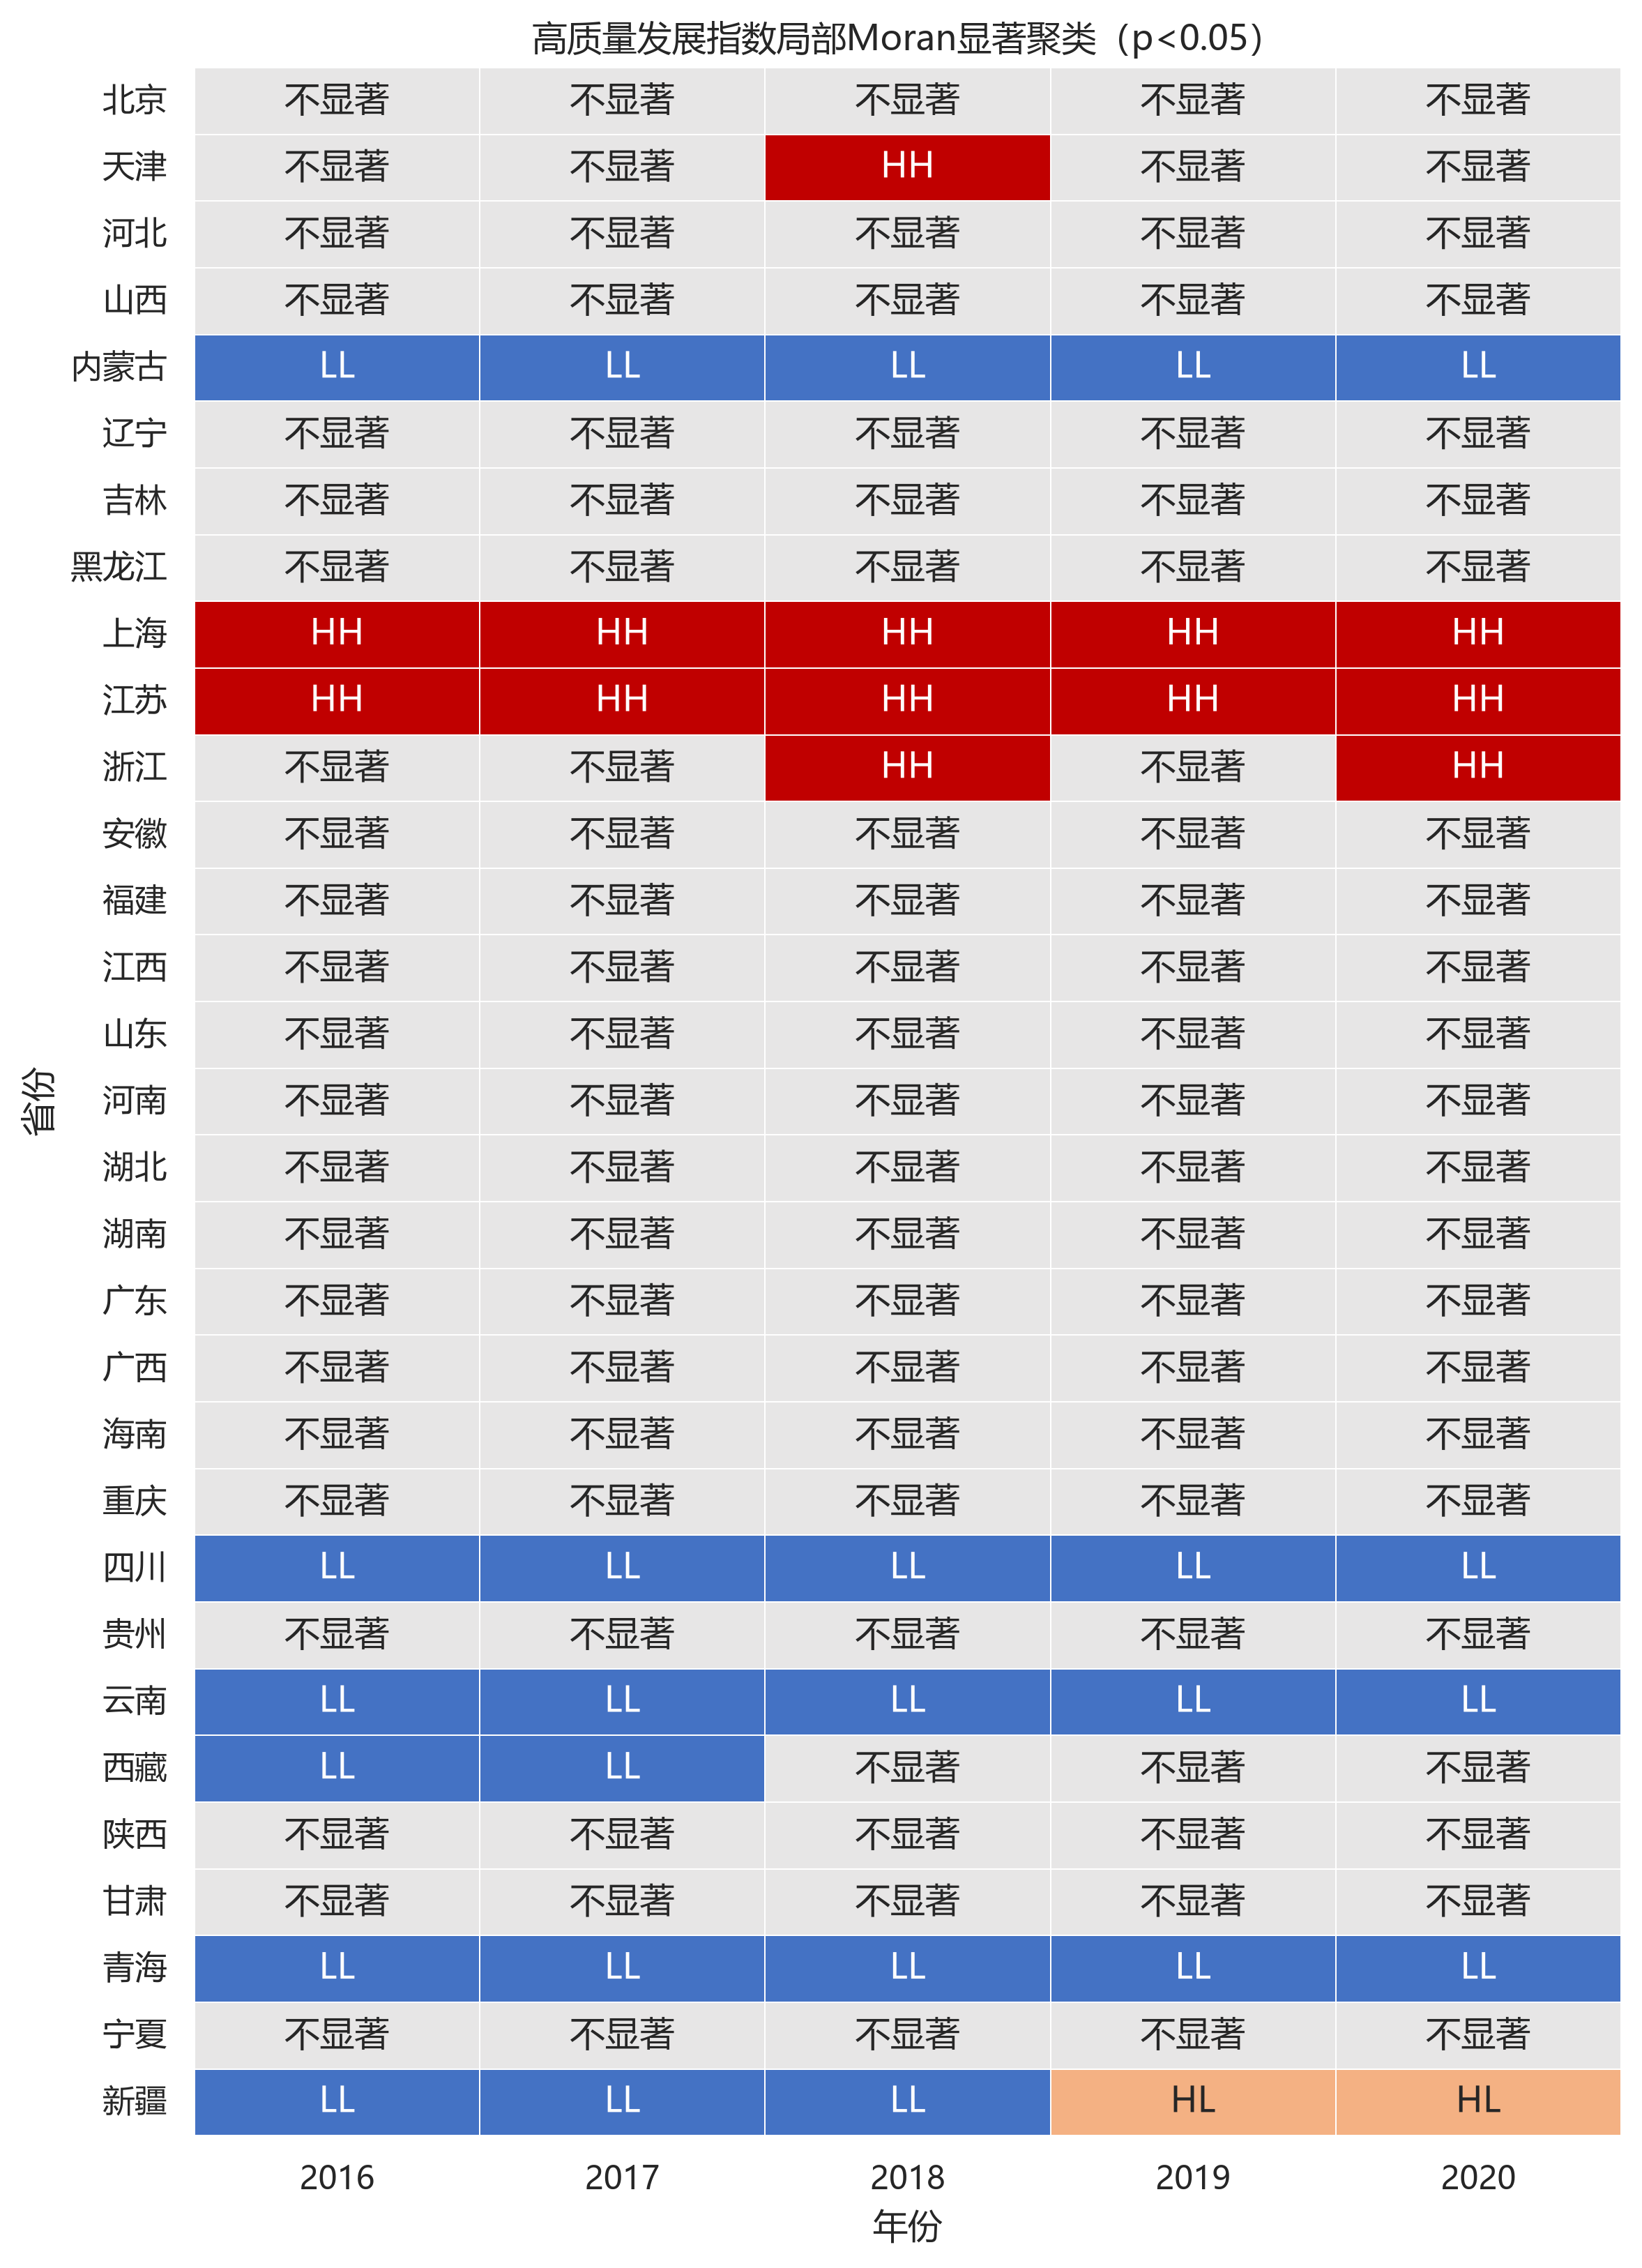
\includegraphics[width=\linewidth,height=0.82\textheight,keepaspectratio]{media/media/image19.png}
\caption*{Figure11 高质量发展指数局部Moran显著聚类}
\end{figure}
\begin{figure}[htbp]
\centering
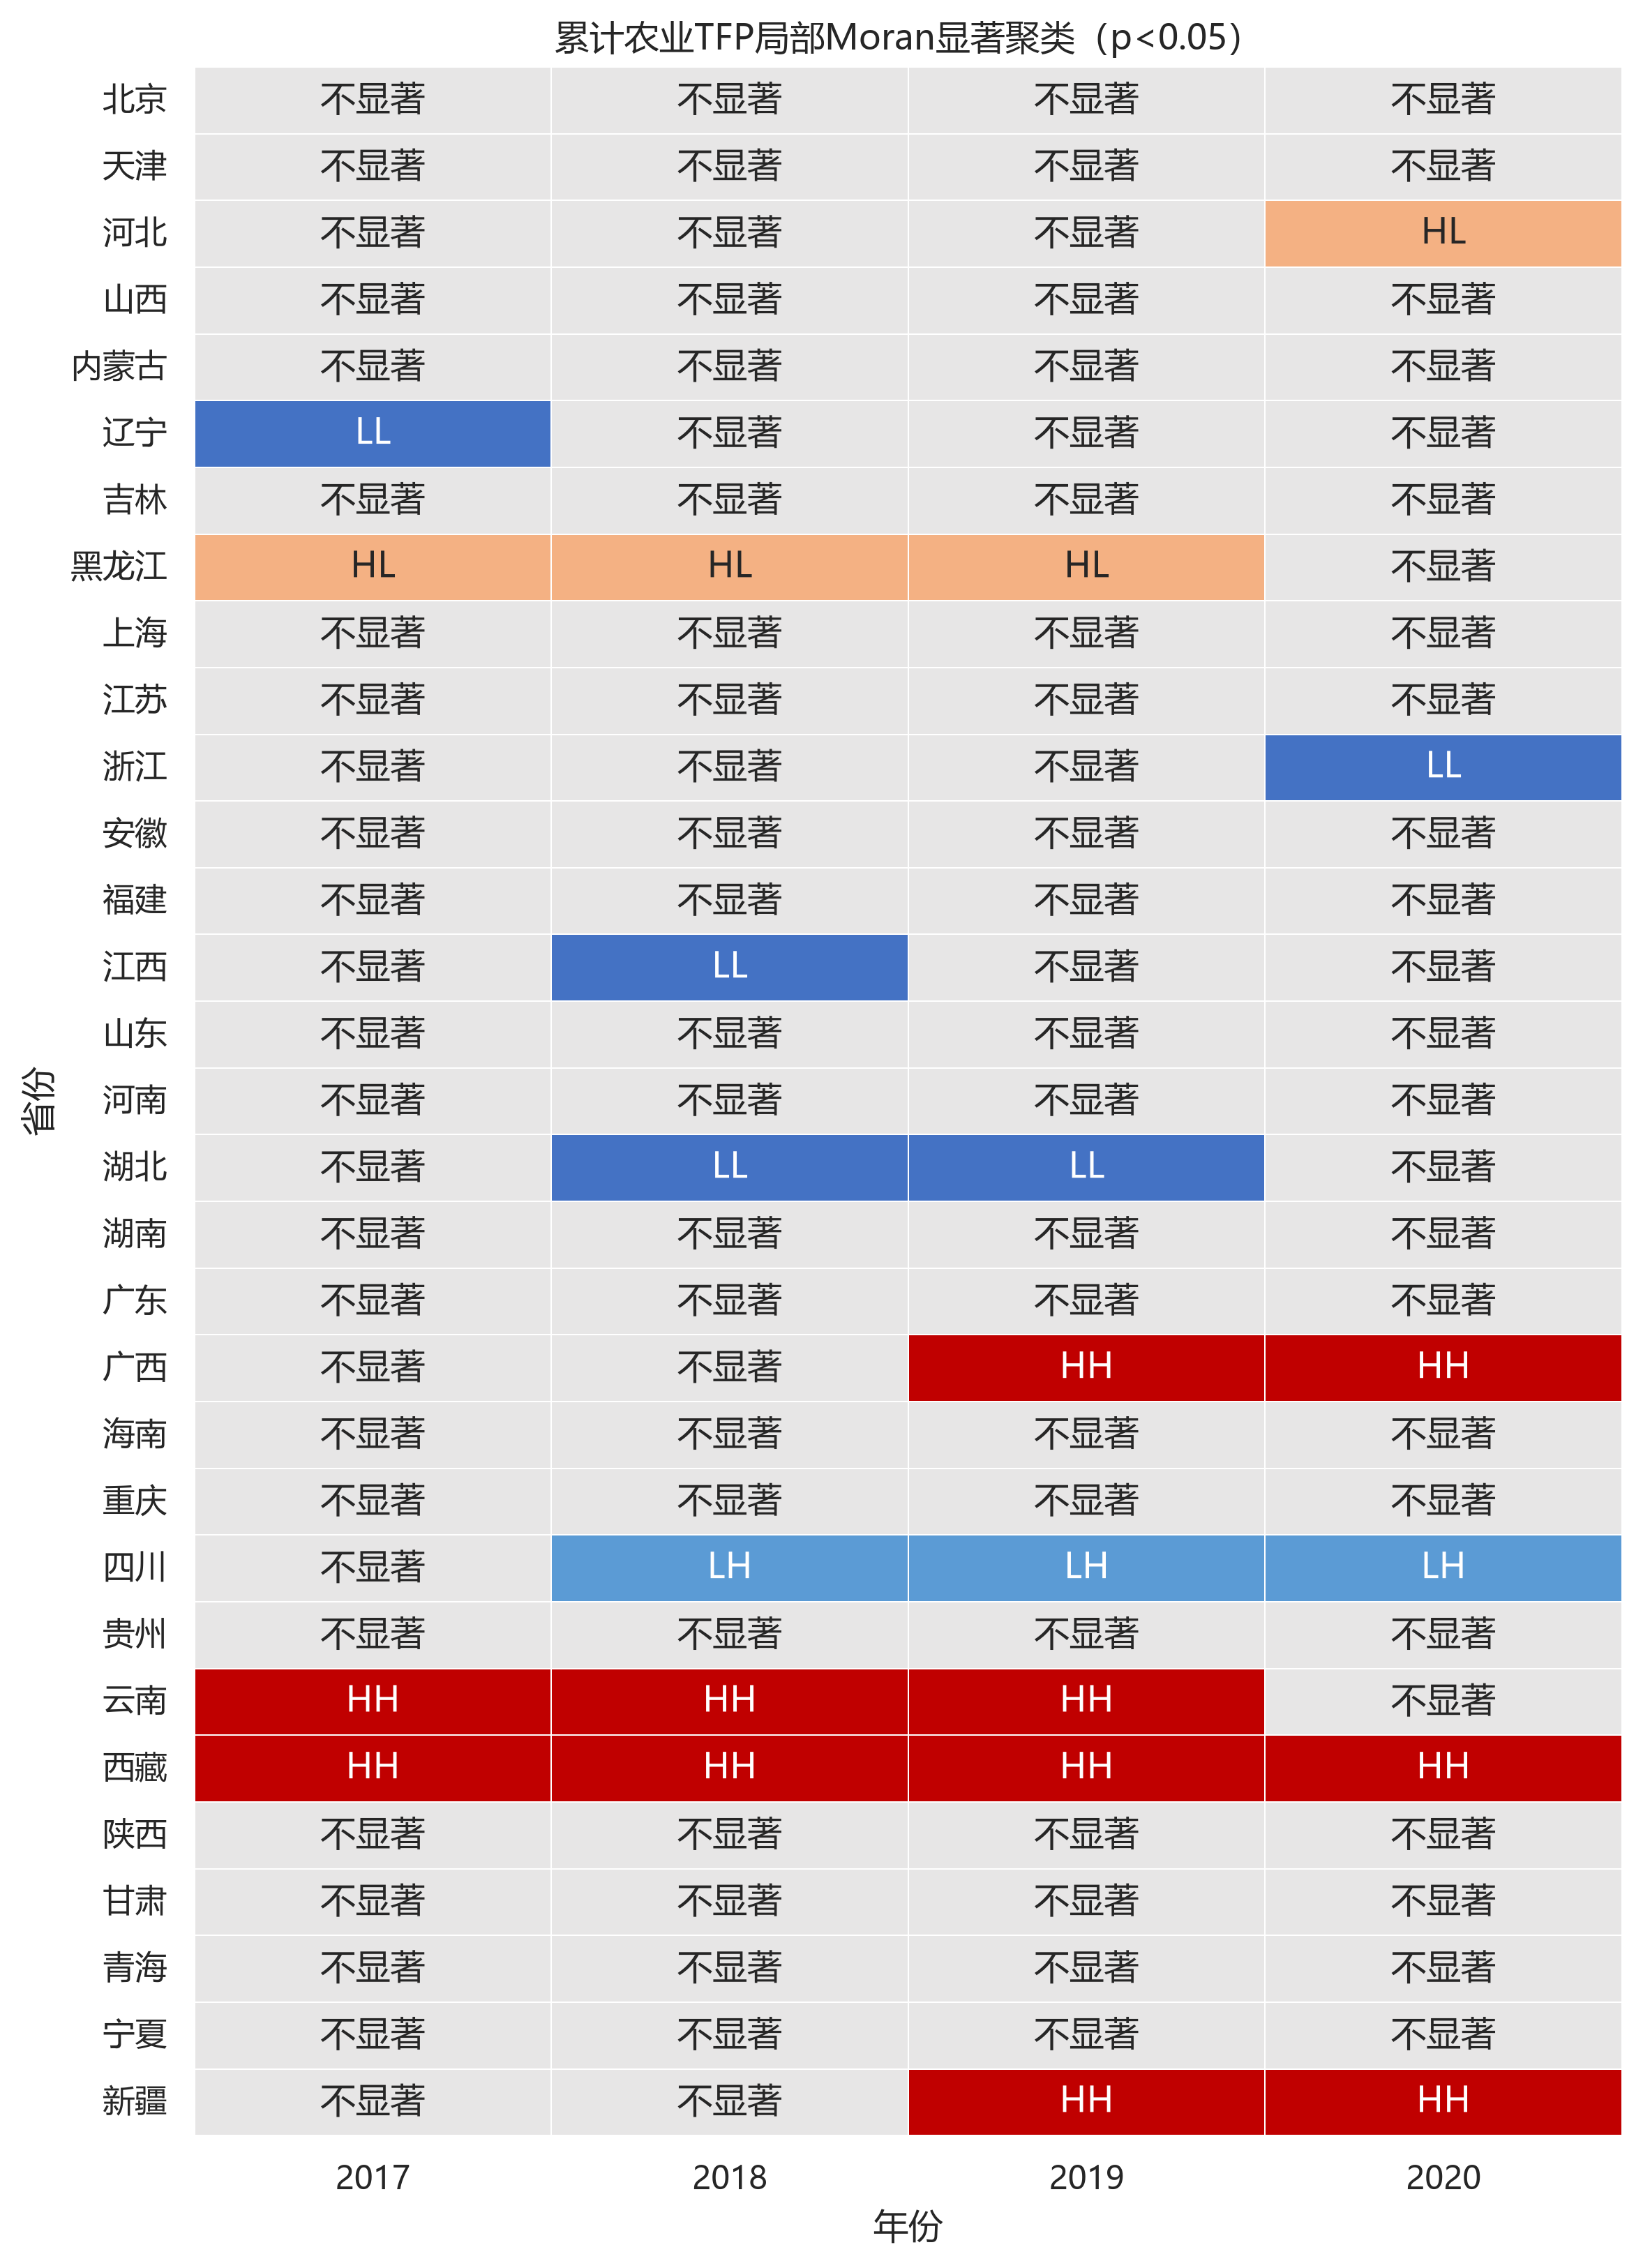
\includegraphics[width=\linewidth,height=0.82\textheight,keepaspectratio]{media/media/image20.png}
\caption*{Figure12 累计农业TFP局部Moran显著聚类}
\end{figure}


\subsection{3.4系统协同性测度}\label{ux7cfbux7edfux534fux540cux6027ux6d4bux5ea6}

\subsubsection{3.4.1耦合协调度}\label{ux8026ux5408ux534fux8c03ux5ea6}

耦合协调度（CCDM）最早起源于物理学用于描述物理电路当中两个及多个模块之间相互作用、能量传递的客观现象，后来广泛应用于区域经济、农业资源与环境等领域的多个系统之间的相互作用强度（耦合度）与良性协同水平（协调度），本文引入耦合协调度模型正是因为该模型使用耦合度阐释若干子系统之间的相互关系，并进一步使用协调发展度对整个系统进行综合评价与研究。 (王淑佳, 以及其他人, 2021)。

本文将农业全要素生产率与经济高质量发展综合指数视为两个独立且相互关联的复合系统：\(U_{1}\)、\(U_{2}\)用以测算二者的耦合协调度\(D\)。该指标可作为后续的空间计量分析的重要部分，用于检验农业全要素生产率与经济高质量发展是否形成良好的互动格局。

农业全要素生产率\(U_{1}\)与经济高质量发展综合指数\(U_{2}\)的构成与先前一致，但值得注意的是由于耦合协调度需要对\(U_{1}\)、\(U_{2}\)两个系统各自进行权重设定，经济高质量发展指数本身是用CRITICS-spearman-\/-熵权法在这里不需要再进行无量纲化和加权处理，但农业全要素生产率使用的DEA-Malmquist方法输出的Malmquist指数(\(M_{0}\))是不能进行无量纲化和加权处理的，所以这里依旧选择是对以2016年为基期累乘出来的累计农业全要素生产率进行相应的处理。

\paragraph{3.4.1.1数据预处理}\label{ux6570ux636eux9884ux5904ux7406}

\[\begin{array}{r}
U_{1,it} = \frac{TFP_{it} - TFP_{\min}}{TFP_{\max} - TFP_{\min}}U_{2,it} = Y_{it}\qquad(14)
\end{array}\]

\noindent \(TFP_{it}\)：第i省第t年的累计全要素生产率（以2016年为基期）。

\noindent \(TFP_{\min},TFP_{\max}\)：全样本中TFP的最小值和最大值（跨年份、跨省份）。

模型对子系统数据的量纲和数字具有敏感性，累计TFP值存在高于1的情况而Y（经济高质量发展综合指数）为0---1的数值，如不处理则会造成耦合协调度的偏误，所以对累计农业全要素生产率\(TFP_{it}\)进行无量纲化处理是很有必要的

\paragraph{3.4.1.2计算耦合度C（Coupling Degree）}\label{ux8ba1ux7b97ux8026ux5408ux5ea6ccoupling-degree}

\[\begin{array}{r}
C_{it} = \sqrt{\frac{U_{1,it} \times U_{2,it}}{\left( \frac{U_{1,it} + U_{2,it}}{2} \right)^{2}}}\qquad(15)
\end{array}\]

耦合协调度测量的是两个系统在动态演化过程中是否同步、关联密度如何是否紧密，即农业全要素生产率与高质量发展综合指数之间除了传统的解释变量对被解释变量的解释效应之外，是否也同时存在被解释变量对解释变量的双向互动，以及这种双向互动的``紧密程度''。

\paragraph{3.4.1.3计算综合协调指数T（Coordination Index）}\label{ux8ba1ux7b97ux7efcux5408ux534fux8c03ux6307ux6570tcoordination-index}

综合协调指数衡量的是解释变量与被解释变量各自的发展水平的整体加权之和，值得点出的是：它反映的是两个系统在彼此相互脱离对方时，单凭借自身所在的``发展水平''譬如经济总量、环境质量分数的加权总和，也可以说是反映解释变量与被解释变量本身的硬实力体现

\[\begin{array}{r}
T_{it} = \alpha \times U_{1,it} + \beta \times U_{2,it}\qquad(16)
\end{array}\]

其中，\(\alpha\)和\(\beta\)是系统间权重，反映两个子系统在协调发展中的相对重要性。

本文假定两个系统同等重要，取：

\[\alpha = \beta = 0.5\]

\paragraph{3.4.1.4计算耦合协调度D（Coupling Coordination Degree）}\label{ux8ba1ux7b97ux8026ux5408ux534fux8c03ux5ea6dcoupling-coordination-degree}

耦合协调度则是在耦合度的基础上，叠加了综合发展指数（T）作为约束。核心机制是构建双重惩罚机制：1.虚假高耦合（耦合度很高，但综合协调指数低如：两变量同步贫困）2.单一的强实力（综合协调指数高但耦合度低）从而保证结果的准确性与可靠性、正确回答解释变量是否真正有效驱动被解释变量的问题。

\[\begin{array}{r}
D_{it} = \sqrt{C_{it} \times T_{it}}\qquad(17)
\end{array}\]

D介于0到1之间，值越大表示TFP与高质量发展综合指数的良性协同水平越高

\begin{longtable}[]{@{}
  >{\centering\arraybackslash}p{(\linewidth - 6\tabcolsep) * \real{0.2500}}
  >{\centering\arraybackslash}p{(\linewidth - 6\tabcolsep) * \real{0.2500}}
  >{\centering\arraybackslash}p{(\linewidth - 6\tabcolsep) * \real{0.2500}}
  >{\centering\arraybackslash}p{(\linewidth - 6\tabcolsep) * \real{0.2500}}@{}}
\toprule\noalign{}
\begin{minipage}[b]{\linewidth}\centering
耦合协调度D区间
\end{minipage} & \begin{minipage}[b]{\linewidth}\centering
协调等级
\end{minipage} & \begin{minipage}[b]{\linewidth}\centering
耦合协调度D区间
\end{minipage} & \begin{minipage}[b]{\linewidth}\centering
协调等级
\end{minipage} \\
\midrule\noalign{}
\endhead
\bottomrule\noalign{}
\endlastfoot
{[}0.00-0.10{]} & 极度失调 & {[}0.50-0.60{]} & 勉强协调 \\
{[}0.10-0.20{]} & 严重失调 & {[}0.60-0.70{]} & 初级协调 \\
{[}0.20-0.30{]} & 中度失调 & {[}0.70-0.80{]} & 中度协调 \\
{[}0.30-0.40{]} & 轻度失调 & {[}0.80-0.90{]} & 良好协调 \\
{[}0.40-0.50{]} & 濒临失调 & {[}0.90-1.00{]} & 优质协调 \\
\end{longtable}
\section{4基准回归}\label{ux57faux51c6ux56deux5f52}

\subsection{4.1基准模型}\label{ux57faux51c6ux6a21ux578b}

为考察农业全要素生产率对经济高质量发展的影响，本文构建如下双向固定效应面板模型：

\[\ln Y_{it} = \alpha + \beta_{1}\ln TFP_{it} + \beta_{2}\ln PopDensity_{it} + \beta_{3}PrimaryShare_{it} + \mu_{i} + \lambda_{t} + \varepsilon_{it}\]

其中：

符号 含义

\(Y_{it}\)：第\(i\)个地区第\(t\)年的高质量发展综合指数。

\(\ln Y_{it}\)：高质量发展指数的自然对数

\(\ln T{FP}_{it}\)：第\(i\)个地区第\(t\)年的农业全要素生产率，DEA-Malmquist 指数累积后取对数

\(\ln PopDensity_{it}\)：第i个地区第\(t\)年的人口密度，常住人口/行政区域面积，取对数

\({PrimaryShare}_{it}\)：第\(i\)个地区第t年的第一产业增加值占GDP比重

\(\mu_{i}\)：地区固定效应，控制不随时间变化的地区特征

\(\lambda_{t}\)：年份固定效应，控制共同时间冲击

\(\varepsilon_{it}\)：随机扰动项

\begin{quote}
\noindent \(a\)：常数项
\end{quote}

\emph{\textbf{Table1控制变量说明与预期符号}}

\begin{longtable}[]{@{}
  >{\centering\arraybackslash}p{(\linewidth - 6\tabcolsep) * \real{0.2500}}
  >{\centering\arraybackslash}p{(\linewidth - 6\tabcolsep) * \real{0.2500}}
  >{\centering\arraybackslash}p{(\linewidth - 6\tabcolsep) * \real{0.2500}}
  >{\centering\arraybackslash}p{(\linewidth - 6\tabcolsep) * \real{0.2500}}@{}}
\toprule\noalign{}
\begin{minipage}[b]{\linewidth}\centering
变量
\end{minipage} & \begin{minipage}[b]{\linewidth}\centering
计算方式
\end{minipage} & \begin{minipage}[b]{\linewidth}\centering
预期方向
\end{minipage} & \begin{minipage}[b]{\linewidth}\centering
控制逻辑
\end{minipage} \\
\midrule\noalign{}
\endhead
\bottomrule\noalign{}
\endlastfoot
人口密度 & 年末常住人口(万人)/土地面积（万平方公里） & 正/负 & 反映人地关系与劳动力丰裕程度 \\
第一产业占比 & 第一产业增加额/GDP & 负或不显著 & 产业结构与农业间的依赖度 \\
\end{longtable}
\emph{\textbf{\hfill\break
}}

\emph{\textbf{Table2基准回归结果}}

\begin{longtable}[]{@{}
  >{\centering\arraybackslash}p{(\linewidth - 12\tabcolsep) * \real{0.1967}}
  >{\centering\arraybackslash}p{(\linewidth - 12\tabcolsep) * \real{0.0338}}
  >{\centering\arraybackslash}p{(\linewidth - 12\tabcolsep) * \real{0.1542}}
  >{\centering\arraybackslash}p{(\linewidth - 12\tabcolsep) * \real{0.1564}}
  >{\centering\arraybackslash}p{(\linewidth - 12\tabcolsep) * \real{0.1386}}
  >{\centering\arraybackslash}p{(\linewidth - 12\tabcolsep) * \real{0.1682}}
  >{\centering\arraybackslash}p{(\linewidth - 12\tabcolsep) * \real{0.1521}}@{}}
\caption{被解释变量：\(\ln Y_{it}\)(高质量发展综合指数)}\tabularnewline
\toprule\noalign{}
\multicolumn{2}{@{}>{\centering\arraybackslash}p{(\linewidth - 12\tabcolsep) * \real{0.2306} + 2\tabcolsep}}{%
\begin{minipage}[b]{\linewidth}\centering
\end{minipage}} & \begin{minipage}[b]{\linewidth}\centering
（1）
\end{minipage} & \begin{minipage}[b]{\linewidth}\centering
（2）
\end{minipage} & \begin{minipage}[b]{\linewidth}\centering
（3）
\end{minipage} & \begin{minipage}[b]{\linewidth}\centering
（4）
\end{minipage} & \begin{minipage}[b]{\linewidth}\centering
（5）
\end{minipage} \\
\midrule\noalign{}
\endfirsthead
\toprule\noalign{}
\multicolumn{2}{@{}>{\centering\arraybackslash}p{(\linewidth - 12\tabcolsep) * \real{0.2306} + 2\tabcolsep}}{%
\begin{minipage}[b]{\linewidth}\centering
\end{minipage}} & \begin{minipage}[b]{\linewidth}\centering
（1）
\end{minipage} & \begin{minipage}[b]{\linewidth}\centering
（2）
\end{minipage} & \begin{minipage}[b]{\linewidth}\centering
（3）
\end{minipage} & \begin{minipage}[b]{\linewidth}\centering
（4）
\end{minipage} & \begin{minipage}[b]{\linewidth}\centering
（5）
\end{minipage} \\
\midrule\noalign{}
\endhead
\bottomrule\noalign{}
\endlastfoot
\multicolumn{2}{@{}>{\centering\arraybackslash}p{(\linewidth - 12\tabcolsep) * \real{0.2306} + 2\tabcolsep}}{%
\(\ln TFP_{it}\)} & -0.019

(0.134)

{[}-0.145{]} & \({0.293}^{**}\)

(0.107)

{[}2.725{]} & \(- {0.279}^{*}\)

(0.163)

{[}-1.714{]} & \({0.716}^{***}\)

(0.118)

{[}6.090{]} & \({0.446}^{**}\)

(0.194)

{[}2.300{]} \\
& \multicolumn{6}{>{\centering\arraybackslash}p{(\linewidth - 12\tabcolsep) * \real{0.8033} + 10\tabcolsep}@{}}{%
} \\
\multicolumn{2}{@{}>{\centering\arraybackslash}p{(\linewidth - 12\tabcolsep) * \real{0.2306} + 2\tabcolsep}}{%
\(\ln PopDensity_{it}\)} & & \({0.140}^{***}\)

(0.030)

{[}4.727{]} & \({0.128}^{***}\)

(0.027)

{[}4.703{]} & -0.644

（1.274）

{[}-0.505{]} & -0.104

(1.342)

{[}-0.077{]} \\
& \multicolumn{6}{>{\centering\arraybackslash}p{(\linewidth - 12\tabcolsep) * \real{0.8033} + 10\tabcolsep}@{}}{%
} \\
\multicolumn{2}{@{}>{\centering\arraybackslash}p{(\linewidth - 12\tabcolsep) * \real{0.2306} + 2\tabcolsep}}{%
\(PrimaryShare_{it}\)} & & \(- {0.017}^{**}\)

(0.007)

{[}-2.405{]} & \(- {0.016}^{**}\)

(0.006)

{[}-2.545{]} & \(- {0.040}^{(**)}\)

（0.018）

{[}-2.293{]} & -0.003

(0.026)

{[}-0.111{]} \\
\multicolumn{2}{@{}>{\centering\arraybackslash}p{(\linewidth - 12\tabcolsep) * \real{0.2306} + 2\tabcolsep}}{%
控制变量} & 否 & 是 & 是 & 是 & 是 \\
\multicolumn{2}{@{}>{\centering\arraybackslash}p{(\linewidth - 12\tabcolsep) * \real{0.2306} + 2\tabcolsep}}{%
省份固定效应} & 否 & 否 & 否 & 是 & 是 \\
\multicolumn{2}{@{}>{\centering\arraybackslash}p{(\linewidth - 12\tabcolsep) * \real{0.2306} + 2\tabcolsep}}{%
年份固定效应} & 否 & 否 & 是 & 否 & 是 \\
\multicolumn{2}{@{}>{\centering\arraybackslash}p{(\linewidth - 12\tabcolsep) * \real{0.2306} + 2\tabcolsep}}{%
观测值} & 155 & 155 & 155 & 155 & 155 \\
\multicolumn{2}{@{}>{\centering\arraybackslash}p{(\linewidth - 12\tabcolsep) * \real{0.2306} + 2\tabcolsep}}{%
省份数} & 31 & 31 & 31 & 31 & 31 \\
\multicolumn{2}{@{}>{\centering\arraybackslash}p{(\linewidth - 12\tabcolsep) * \real{0.2306} + 2\tabcolsep}}{%
\(R^{2}\)} & 0.000 & 0.591 & 0.662 & 0.948 & 0.957 \\
\multicolumn{2}{@{}>{\centering\arraybackslash}p{(\linewidth - 12\tabcolsep) * \real{0.2306} + 2\tabcolsep}}{%
调整后\(R^{2}\)} & -0.006 & 0.583 & 0.646 & 0.934 & 0.943 \\
\end{longtable}

注：\(*\)p\textless0.1,**p\textless0.05,***p\textless0.01,括号内为省份层面聚类稳健标准误，方括号内为t统计量

Table2报告了逐步加入控制变量和固定效应的递进估计结果。第（1）列仅以\\
\(\ln TFP_{it}\)对\(\ln Y_{it}\)进行OLS回归，系数仅为-0.019且不显著，调整后的\(R^{2}\)为负，模型设定极不充分。第（2）列加入控制变量后，系数变为0.293（p\textless0.05）调整后的\(R^{2}\)升至0.583，表明控制变量对模型解释力有重要贡献。第（3）列仅控制年份固定效应而不控制省份固定效应时，系数为-0.279（p\textless0.1）,说明忽略省份异质性会导致估计偏差甚至方向逆转。第（4）列控制省份固定效应后，系数变至0.716，调整后的\(R^{2}\)达到0.934，表明省份间不可观测的固定差异是更主要的遗漏变量来源，进行省份固定是建模的关键。第（5）列则同时进行控制双向固定效应，系数为0.446（p\textless0.05）,调整后的\(R^{2}\)进一步升为0.943。核心解释变量在控制省份固定效应后始终显著为正，验证了农业全要素生产率对高质量发展的稳健促进作用。第（3）列与第（4）列的对比清晰表明，忽略省份固定效应会严重低估甚至颠倒农业全要素生产率的真实效应，因此本文以双向固定效应模型作为基准是合理的。

\subsection{4.2稳健性检验}\label{ux7a33ux5065ux6027ux68c0ux9a8c}

为避免基准结论受到极端值、特殊行政单元、同期性、函数形式和标准误设定的驱动，本文依次进行双侧1\%缩尾、剔除四个直辖市、核心解释变量滞后一期、水平值估计以及Driscoll---Kraay标准误检验。除特别说明外，各模型均控制人口密度、第一产业占比以及省份和年份固定效应。

\begin{longtable}[]{@{}
  >{\centering\arraybackslash}p{(\linewidth - 8\tabcolsep) * \real{0.3745}}
  >{\centering\arraybackslash}p{(\linewidth - 8\tabcolsep) * \real{0.1568}}
  >{\centering\arraybackslash}p{(\linewidth - 8\tabcolsep) * \real{0.1481}}
  >{\centering\arraybackslash}p{(\linewidth - 8\tabcolsep) * \real{0.0958}}
  >{\centering\arraybackslash}p{(\linewidth - 8\tabcolsep) * \real{0.1481}}@{}}
\caption{表5 稳健性检验结果}\tabularnewline
\toprule\noalign{}
\begin{minipage}[b]{\linewidth}\centering
\textbf{模型}
\end{minipage} & \begin{minipage}[b]{\linewidth}\centering
\textbf{TFP系数}
\end{minipage} & \begin{minipage}[b]{\linewidth}\centering
\textbf{标准误}
\end{minipage} & \begin{minipage}[b]{\linewidth}\centering
\textbf{N}
\end{minipage} & \begin{minipage}[b]{\linewidth}\centering
\textbf{组内R²}
\end{minipage} \\
\midrule\noalign{}
\endfirsthead
\toprule\noalign{}
\begin{minipage}[b]{\linewidth}\centering
\textbf{模型}
\end{minipage} & \begin{minipage}[b]{\linewidth}\centering
\textbf{TFP系数}
\end{minipage} & \begin{minipage}[b]{\linewidth}\centering
\textbf{标准误}
\end{minipage} & \begin{minipage}[b]{\linewidth}\centering
\textbf{N}
\end{minipage} & \begin{minipage}[b]{\linewidth}\centering
\textbf{组内R²}
\end{minipage} \\
\midrule\noalign{}
\endhead
\bottomrule\noalign{}
\endlastfoot
基准：双向固定效应 & 0.446** & (0.191) & 155 & 0.526 \\
双侧1\%缩尾 & 0.382** & (0.147) & 155 & 0.502 \\
剔除四个直辖市 & 0.493** & (0.201) & 135 & 0.586 \\
解释变量滞后一期 & 0.255* & (0.152) & 124 & 0.348 \\
水平值函数形式 & 0.043 & (0.030) & 155 & 0.258 \\
Driscoll-Kraay标准误 & 0.446*** & (0.091) & 155 & 0.526 \\
\end{longtable}

注：括号内为标准误；*、**、***分别表示在10\%、5\%和1\%水平上显著。

对数基准模型中TFP系数为0.446，并在5\%水平显著。缩尾处理和剔除直辖市后，系数分别为0.382和0.493，均保持显著为正；采用Driscoll---Kraay标准误后结论亦未改变。滞后一期TFP的系数为0.255，在10\%水平弱显著，说明促进作用可能具有一定时滞。水平值模型的系数为0.043，但未达到常用显著性水平，意味着结论对函数形式并非完全不敏感。总体而言，正向影响在主要对数设定和样本调整下较为稳定，但不应将稳健性表述为对所有函数形式均成立。


\begin{figure}[htbp]
\centering
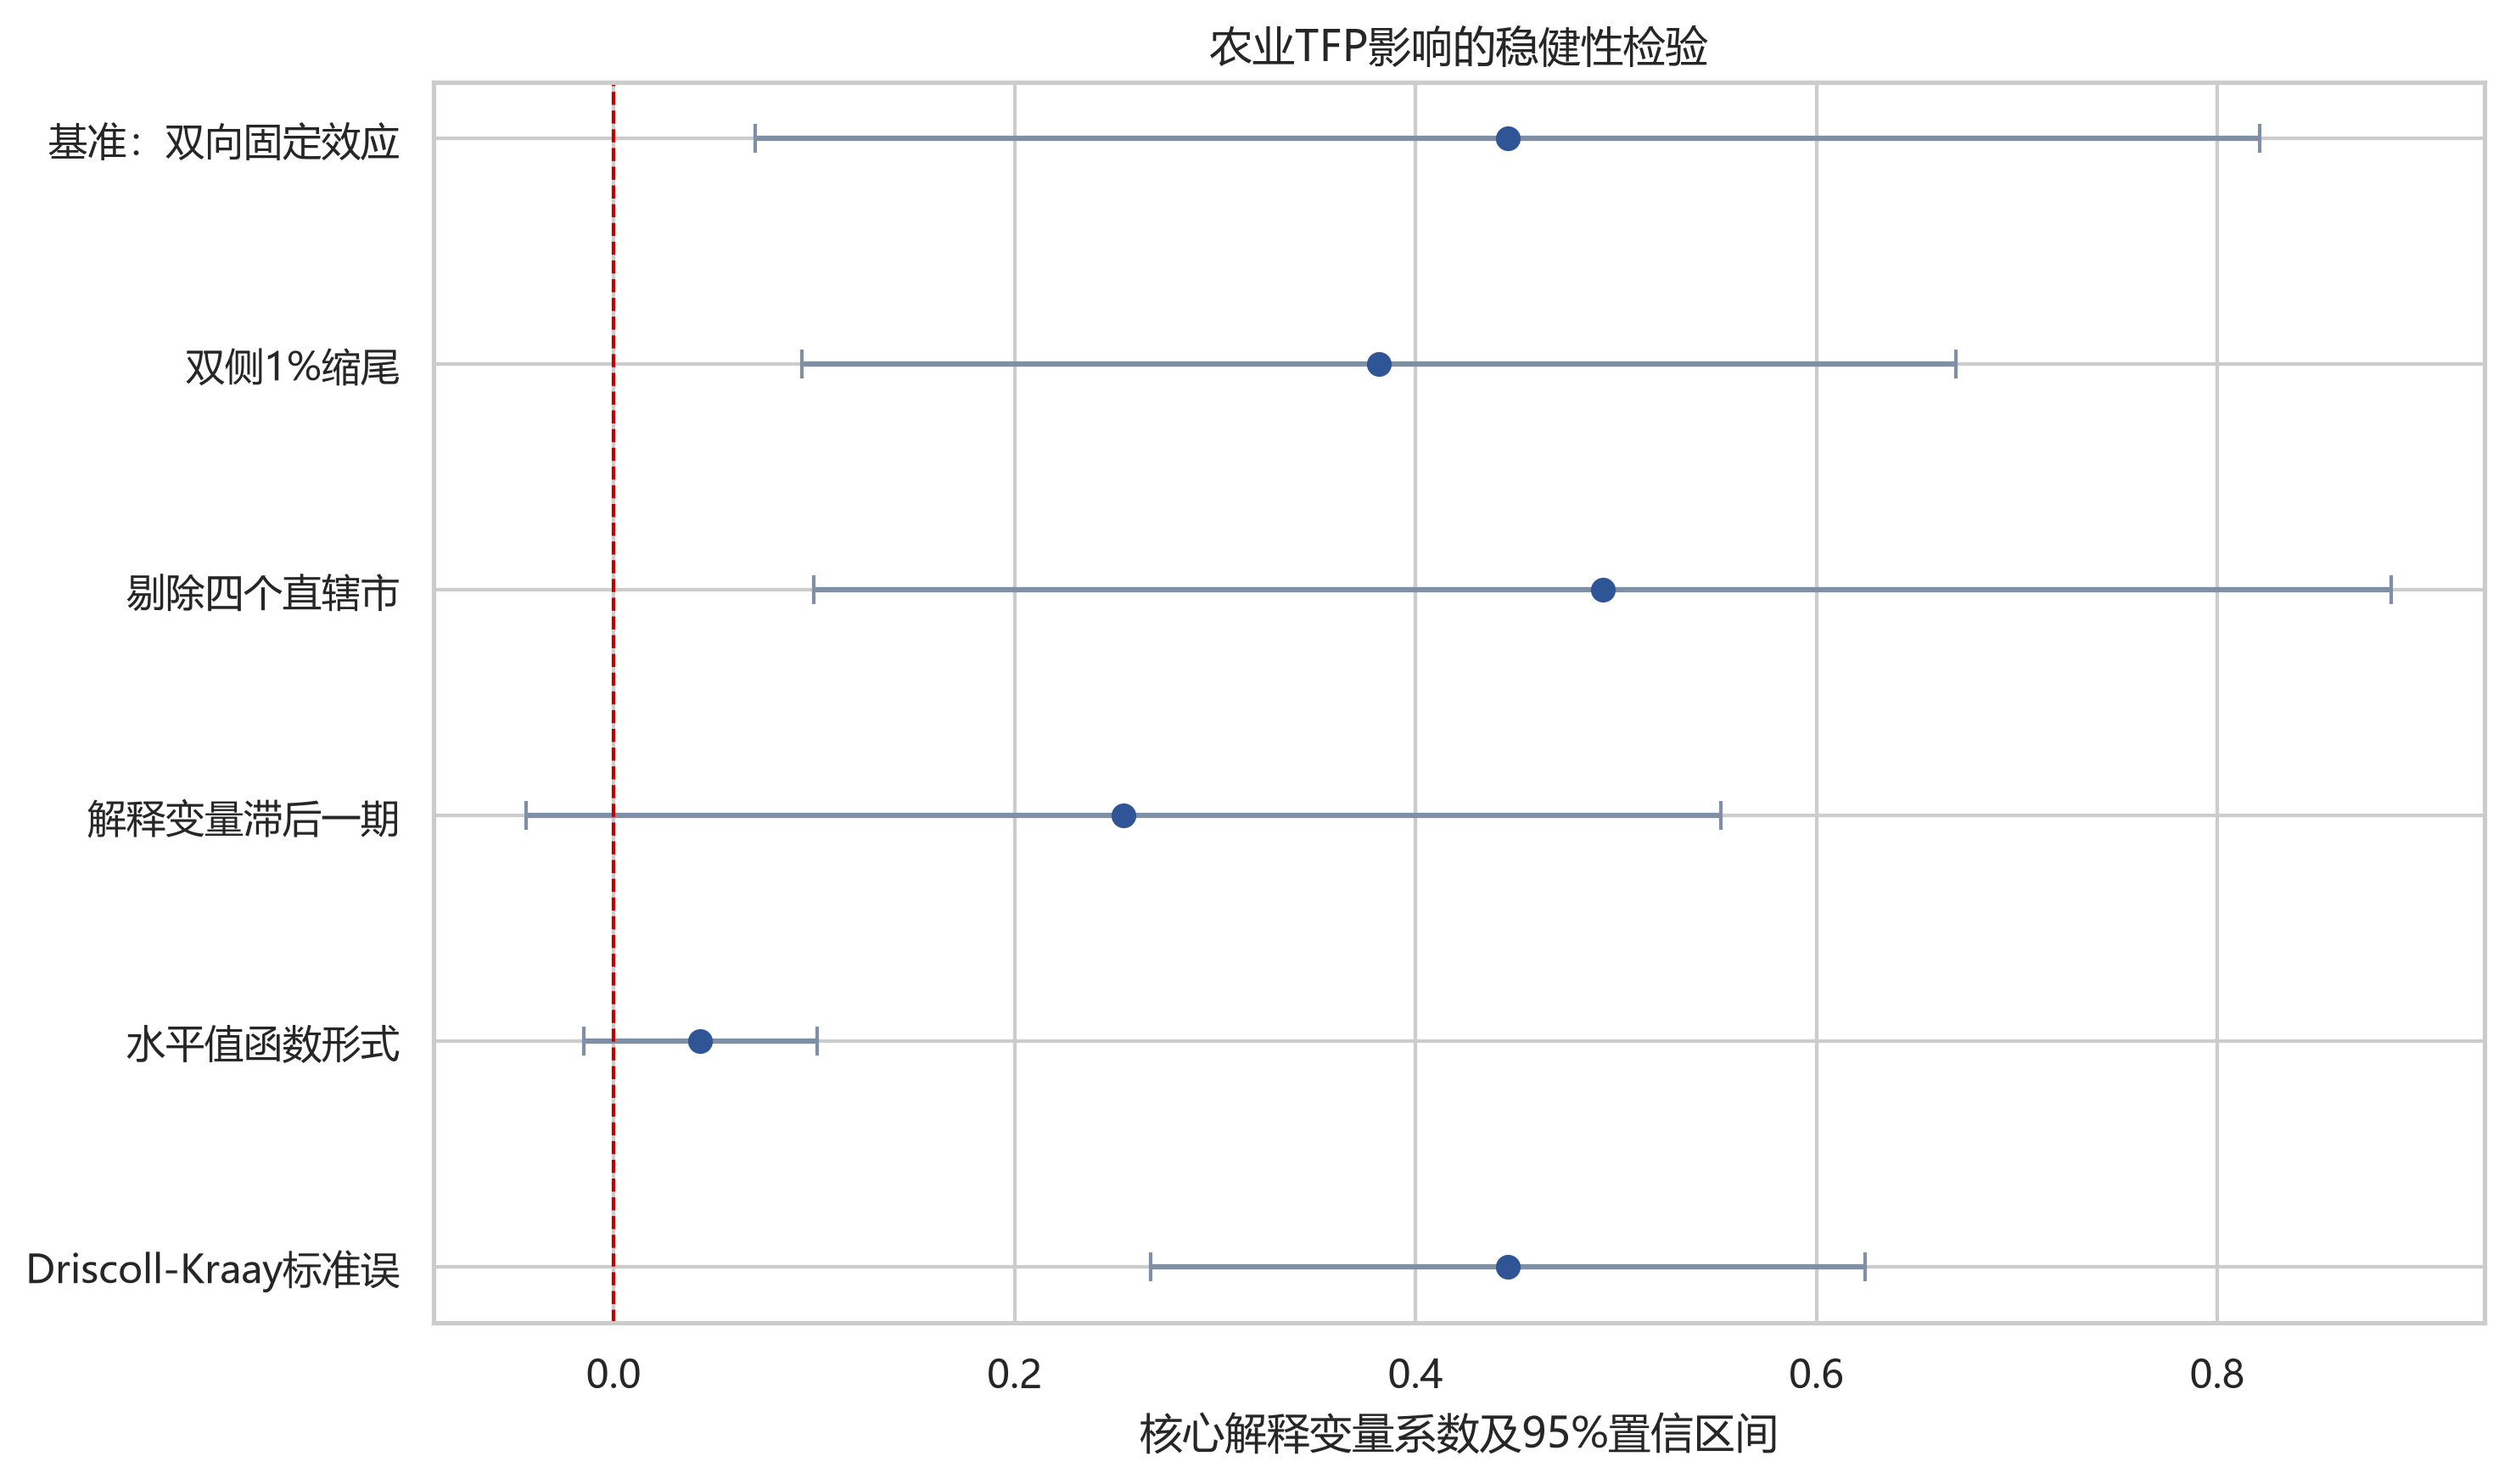
\includegraphics[width=\linewidth,height=0.82\textheight,keepaspectratio]{media/media/image21.png}
\caption*{Figure13 农业TFP影响的稳健性检验}
\end{figure}


\subsection{4.3内生性检验}\label{ux5185ux751fux6027ux68c0ux9a8c}

农业TFP与高质量发展之间可能存在反向作用，同时遗漏的制度与技术冲击也可能影响二者。受样本期较短且缺乏可信外部冲击变量的限制，本文采用农业TFP的一期滞后作为内部工具变量进行双向固定效应2SLS估计。其识别要求是：滞后TFP与当期TFP相关，并在控制省份、年份和控制变量后不通过其他持续性渠道直接影响当期高质量发展。该排除限制无法由数据完全检验，因此本节属于缓解性而非决定性因果识别。

\[\text{第一阶段：}\quad \ln TFP_{it}=\pi\ln TFP_{i,t-1}+\gamma X_{it}+\mu_i+\lambda_t+\nu_{it}\]

\[\text{第二阶段：}\quad \ln Y_{it}=\beta\widehat{\ln TFP}_{it}+\delta X_{it}+\mu_i+\lambda_t+\varepsilon_{it}\]

\begin{longtable}[]{@{}
  >{\centering\arraybackslash}p{(\linewidth - 10\tabcolsep) * \real{0.3017}}
  >{\centering\arraybackslash}p{(\linewidth - 10\tabcolsep) * \real{0.1466}}
  >{\centering\arraybackslash}p{(\linewidth - 10\tabcolsep) * \real{0.1379}}
  >{\centering\arraybackslash}p{(\linewidth - 10\tabcolsep) * \real{0.0862}}
  >{\centering\arraybackslash}p{(\linewidth - 10\tabcolsep) * \real{0.1724}}
  >{\centering\arraybackslash}p{(\linewidth - 10\tabcolsep) * \real{0.1552}}@{}}
\caption{表6 内生性检验：一期滞后内部工具变量}\tabularnewline
\toprule\noalign{}
\begin{minipage}[b]{\linewidth}\centering
\textbf{模型}
\end{minipage} & \begin{minipage}[b]{\linewidth}\centering
\textbf{TFP系数}
\end{minipage} & \begin{minipage}[b]{\linewidth}\centering
\textbf{标准误}
\end{minipage} & \begin{minipage}[b]{\linewidth}\centering
\textbf{N}
\end{minipage} & \begin{minipage}[b]{\linewidth}\centering
\textbf{第一阶段F}
\end{minipage} & \begin{minipage}[b]{\linewidth}\centering
\textbf{DWH p值}
\end{minipage} \\
\midrule\noalign{}
\endfirsthead
\toprule\noalign{}
\begin{minipage}[b]{\linewidth}\centering
\textbf{模型}
\end{minipage} & \begin{minipage}[b]{\linewidth}\centering
\textbf{TFP系数}
\end{minipage} & \begin{minipage}[b]{\linewidth}\centering
\textbf{标准误}
\end{minipage} & \begin{minipage}[b]{\linewidth}\centering
\textbf{N}
\end{minipage} & \begin{minipage}[b]{\linewidth}\centering
\textbf{第一阶段F}
\end{minipage} & \begin{minipage}[b]{\linewidth}\centering
\textbf{DWH p值}
\end{minipage} \\
\midrule\noalign{}
\endhead
\bottomrule\noalign{}
\endlastfoot
同样本双向固定效应OLS & 0.396*** & (0.145) & 124 & --- & --- \\
2SLS内部工具变量 & 0.526* & (0.271) & 124 & 39.36 & 0.401 \\
\end{longtable}

注：括号内为省份聚类稳健标准误；*、**、***分别表示在10\%、5\%和1\%水平上显著。

第一阶段部分F统计量为39.36，显著高于经验阈值10，未显示明显弱工具变量问题。2SLS估计系数为0.526，p值为0.055，在10\%水平显著为正，与基准回归方向一致且数值略大。Wu---Hausman检验p值为0.401，不能拒绝解释变量外生的原假设，说明样本内没有强证据表明OLS存在显著内生性偏误。结合工具变量排除限制无法完全验证这一事实，本文将IV结果视为支持性证据，而不作严格因果宣称。


\begin{figure}[htbp]
\centering
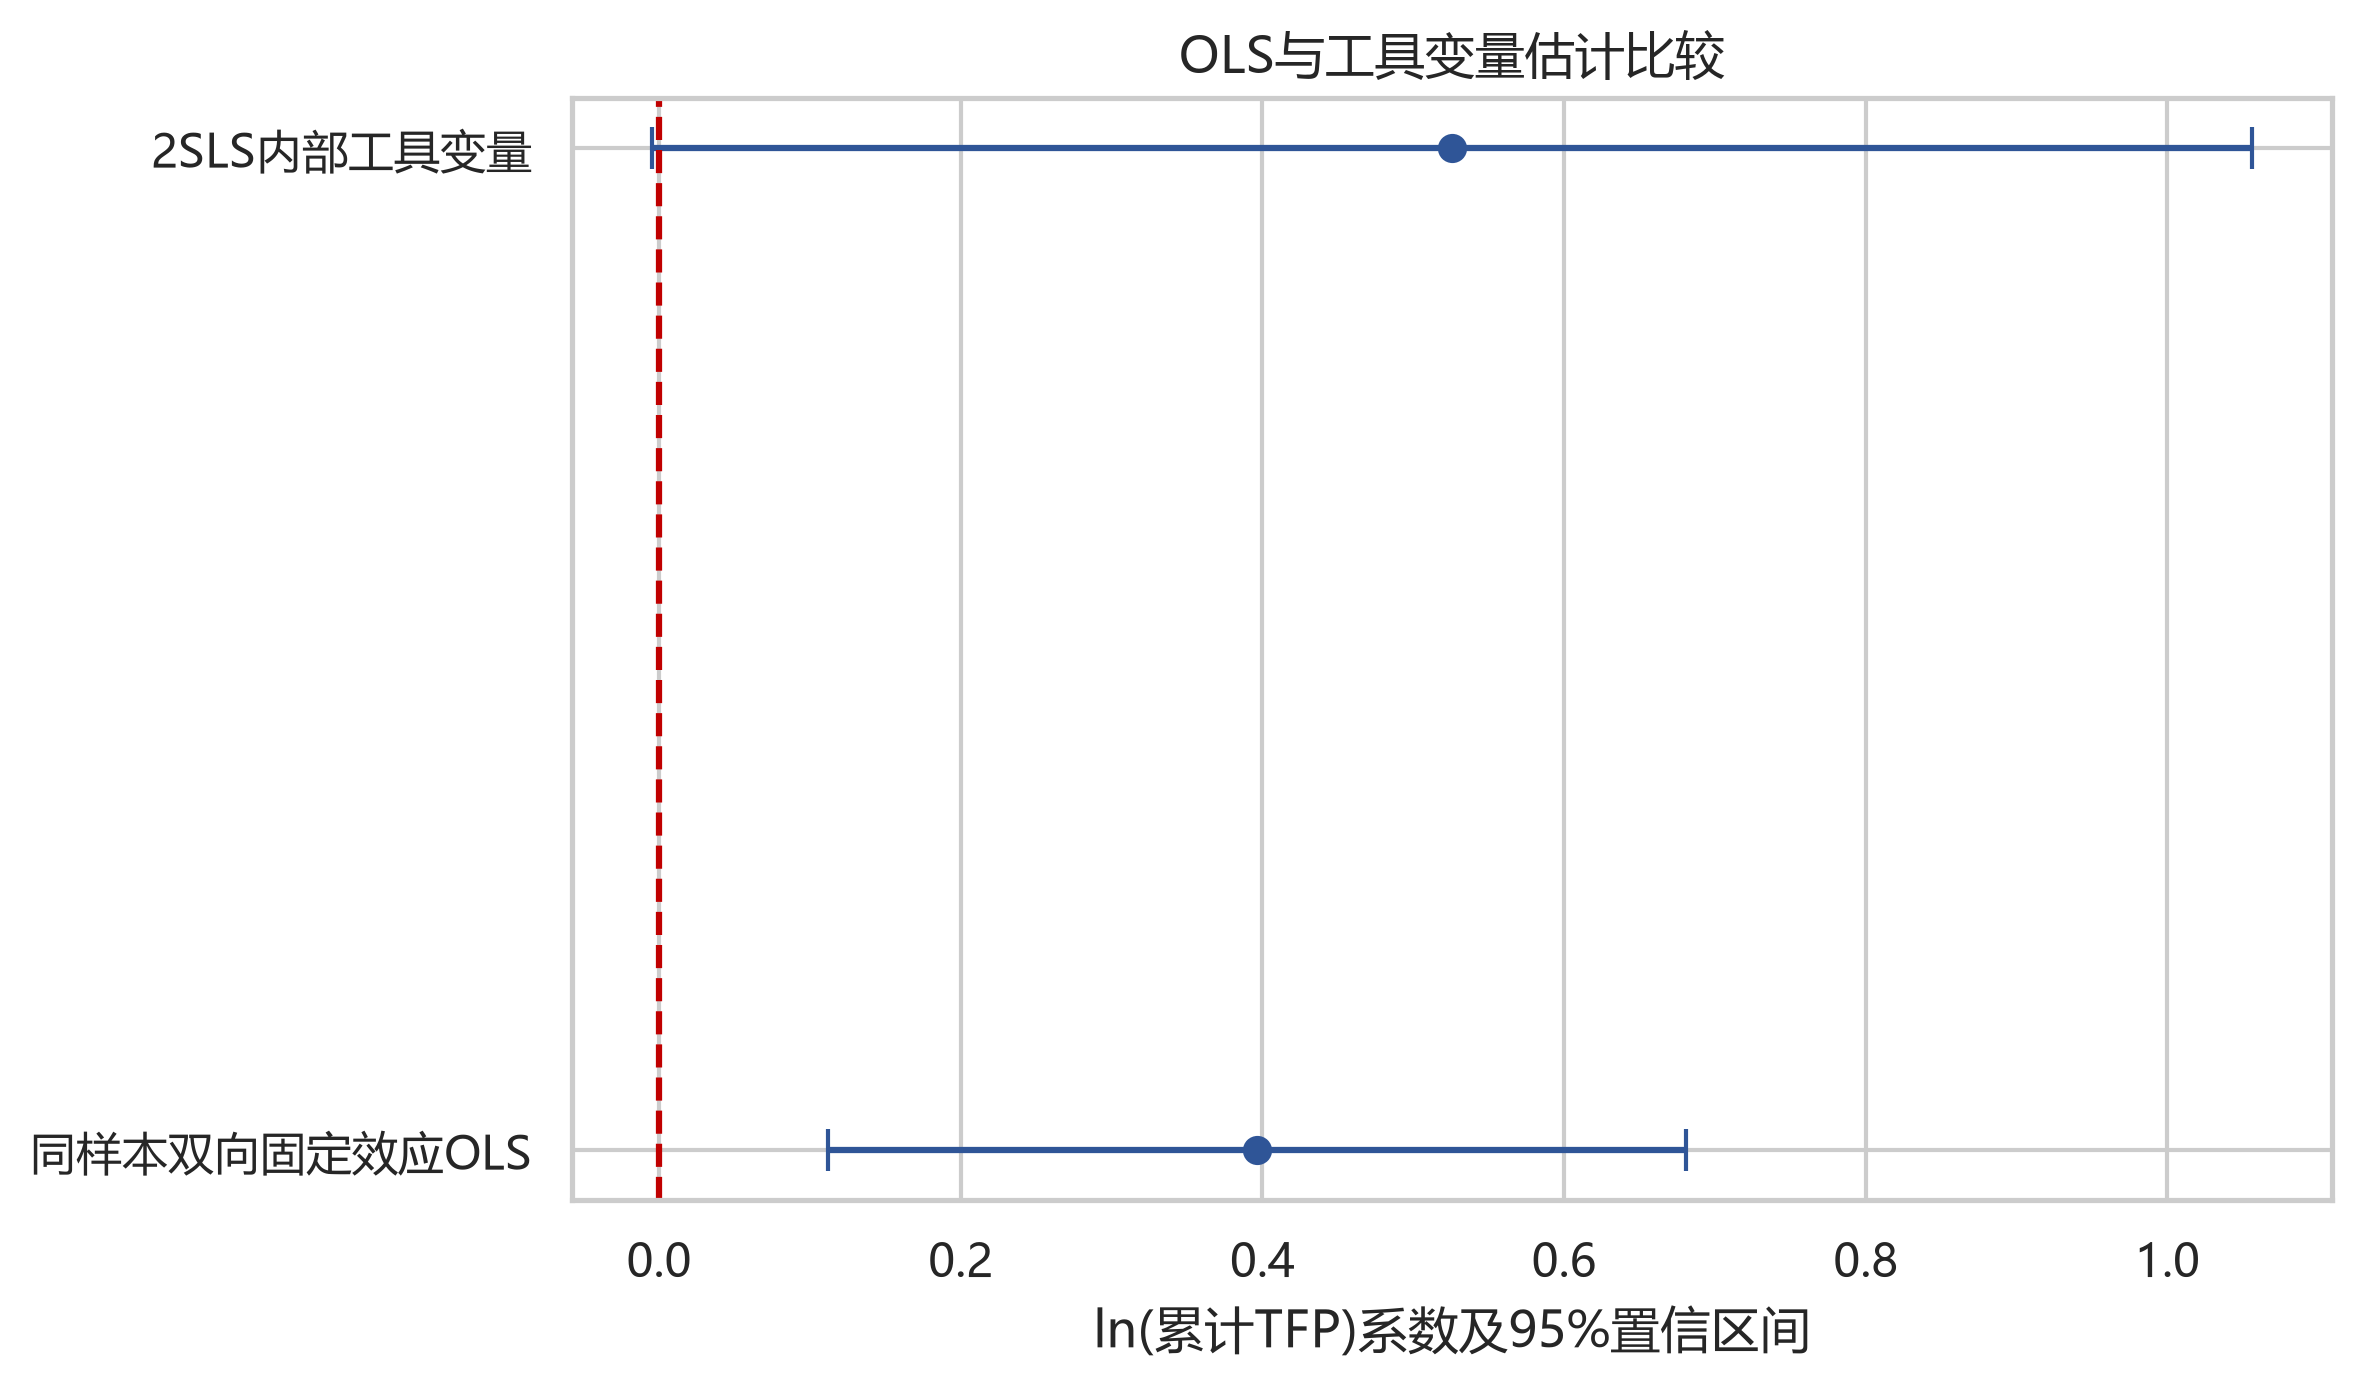
\includegraphics[width=\linewidth,height=0.82\textheight,keepaspectratio]{media/media/image22.png}
\caption*{Figure14 OLS与工具变量估计结果比较}
\end{figure}


\section{5模型应用与结果}\label{ux6a21ux578bux5e94ux7528ux4e0eux7ed3ux679c}

\subsection{5.1空间溢出效应}\label{ux7a7aux95f4ux6ea2ux51faux6548ux5e94}

全局Moran检验表明高质量发展存在稳定空间依赖，因此使用非空间面板模型可能忽略邻近地区的联动。本文采用同时包含被解释变量空间滞后项和解释变量空间滞后项的空间杜宾模型（SDM）：

\[\ln Y_{it}=\rho\sum_jw_{ij}\ln Y_{jt}+\beta\ln TFP_{it}+\theta\sum_jw_{ij}\ln TFP_{jt}+\gamma X_{it}+\eta WX_{it}+\mu_i+\lambda_t+\varepsilon_{it}\]

模型采用省级接壤权重并控制省份固定效应和年份虚拟变量。由于存在空间反馈，β和θ不能直接解释为最终边际效应，需根据偏微分矩阵\(S=(I-\rho W)^{-1}(\beta I+\theta W)\)分解为直接效应、间接效应和总效应。

\begin{longtable}[]{@{}
  >{\centering\arraybackslash}p{(\linewidth - 6\tabcolsep) * \real{0.4263}}
  >{\centering\arraybackslash}p{(\linewidth - 6\tabcolsep) * \real{0.1914}}
  >{\centering\arraybackslash}p{(\linewidth - 6\tabcolsep) * \real{0.1218}}
  >{\centering\arraybackslash}p{(\linewidth - 6\tabcolsep) * \real{0.1218}}@{}}
\caption{表7 空间杜宾模型约束检验}\tabularnewline
\toprule\noalign{}
\begin{minipage}[b]{\linewidth}\centering
\textbf{原假设}
\end{minipage} & \begin{minipage}[b]{\linewidth}\centering
\textbf{Wald统计量}
\end{minipage} & \begin{minipage}[b]{\linewidth}\centering
\textbf{自由度}
\end{minipage} & \begin{minipage}[b]{\linewidth}\centering
\textbf{p值}
\end{minipage} \\
\midrule\noalign{}
\endfirsthead
\toprule\noalign{}
\begin{minipage}[b]{\linewidth}\centering
\textbf{原假设}
\end{minipage} & \begin{minipage}[b]{\linewidth}\centering
\textbf{Wald统计量}
\end{minipage} & \begin{minipage}[b]{\linewidth}\centering
\textbf{自由度}
\end{minipage} & \begin{minipage}[b]{\linewidth}\centering
\textbf{p值}
\end{minipage} \\
\midrule\noalign{}
\endhead
\bottomrule\noalign{}
\endlastfoot
SDM简化为SAR & 6.325 & 3 & 0.097 \\
SDM简化为SEM & 8.690 & 3 & 0.034 \\
\end{longtable}

注：SDM→SAR检验空间滞后解释变量系数是否联合为0；SDM→SEM检验共同因子约束。

\begin{longtable}[]{@{}
  >{\centering\arraybackslash}p{(\linewidth - 6\tabcolsep) * \real{0.3480}}
  >{\centering\arraybackslash}p{(\linewidth - 6\tabcolsep) * \real{0.1740}}
  >{\centering\arraybackslash}p{(\linewidth - 6\tabcolsep) * \real{0.1740}}
  >{\centering\arraybackslash}p{(\linewidth - 6\tabcolsep) * \real{0.1392}}@{}}
\caption{表8 空间杜宾模型与TFP效应分解}\tabularnewline
\toprule\noalign{}
\begin{minipage}[b]{\linewidth}\centering
\textbf{变量/效应}
\end{minipage} & \begin{minipage}[b]{\linewidth}\centering
\textbf{估计值}
\end{minipage} & \begin{minipage}[b]{\linewidth}\centering
\textbf{标准误}
\end{minipage} & \begin{minipage}[b]{\linewidth}\centering
\textbf{p值}
\end{minipage} \\
\midrule\noalign{}
\endfirsthead
\toprule\noalign{}
\begin{minipage}[b]{\linewidth}\centering
\textbf{变量/效应}
\end{minipage} & \begin{minipage}[b]{\linewidth}\centering
\textbf{估计值}
\end{minipage} & \begin{minipage}[b]{\linewidth}\centering
\textbf{标准误}
\end{minipage} & \begin{minipage}[b]{\linewidth}\centering
\textbf{p值}
\end{minipage} \\
\midrule\noalign{}
\endhead
\bottomrule\noalign{}
\endlastfoot
lnTFP & 0.355*** & (0.087) & 0.000 \\
W×lnTFP & 0.166 & (0.183) & 0.365 \\
空间滞后系数ρ & 0.216** & (0.102) & 0.035 \\
直接效应 & 0.368*** & (0.086) & 0.000 \\
间接效应 & 0.297 & (0.213) & 0.164 \\
总效应 & 0.665*** & (0.232) & 0.004 \\
\end{longtable}

注：效应分解标准误由参数模拟获得；*、**、***分别表示在10\%、5\%和1\%水平上显著。

空间滞后系数ρ为0.216，并在5\%水平显著，说明本地高质量发展会受到邻近省份高质量发展水平的正向影响。SDM简化为SEM的共同因子约束在5\%水平被拒绝；空间滞后解释变量联合为0的约束在5\%水平不能拒绝、但在10\%水平被拒绝，因此保留一般SDM并报告偏微分效应，同时对间接效应作保守解释。

TFP的直接效应为0.368且在1\%水平显著，总效应为0.665且在1\%水平显著，说明农业生产率提高主要通过本地渠道推动高质量发展。间接效应为0.297，但p值为0.164，置信区间包含0，尚不能确认邻近省份TFP对本地高质量发展产生稳定溢出。由此，H3关于高质量发展空间联动的部分得到支持，但关于TFP跨省间接溢出的证据不足。


\begin{figure}[htbp]
\centering
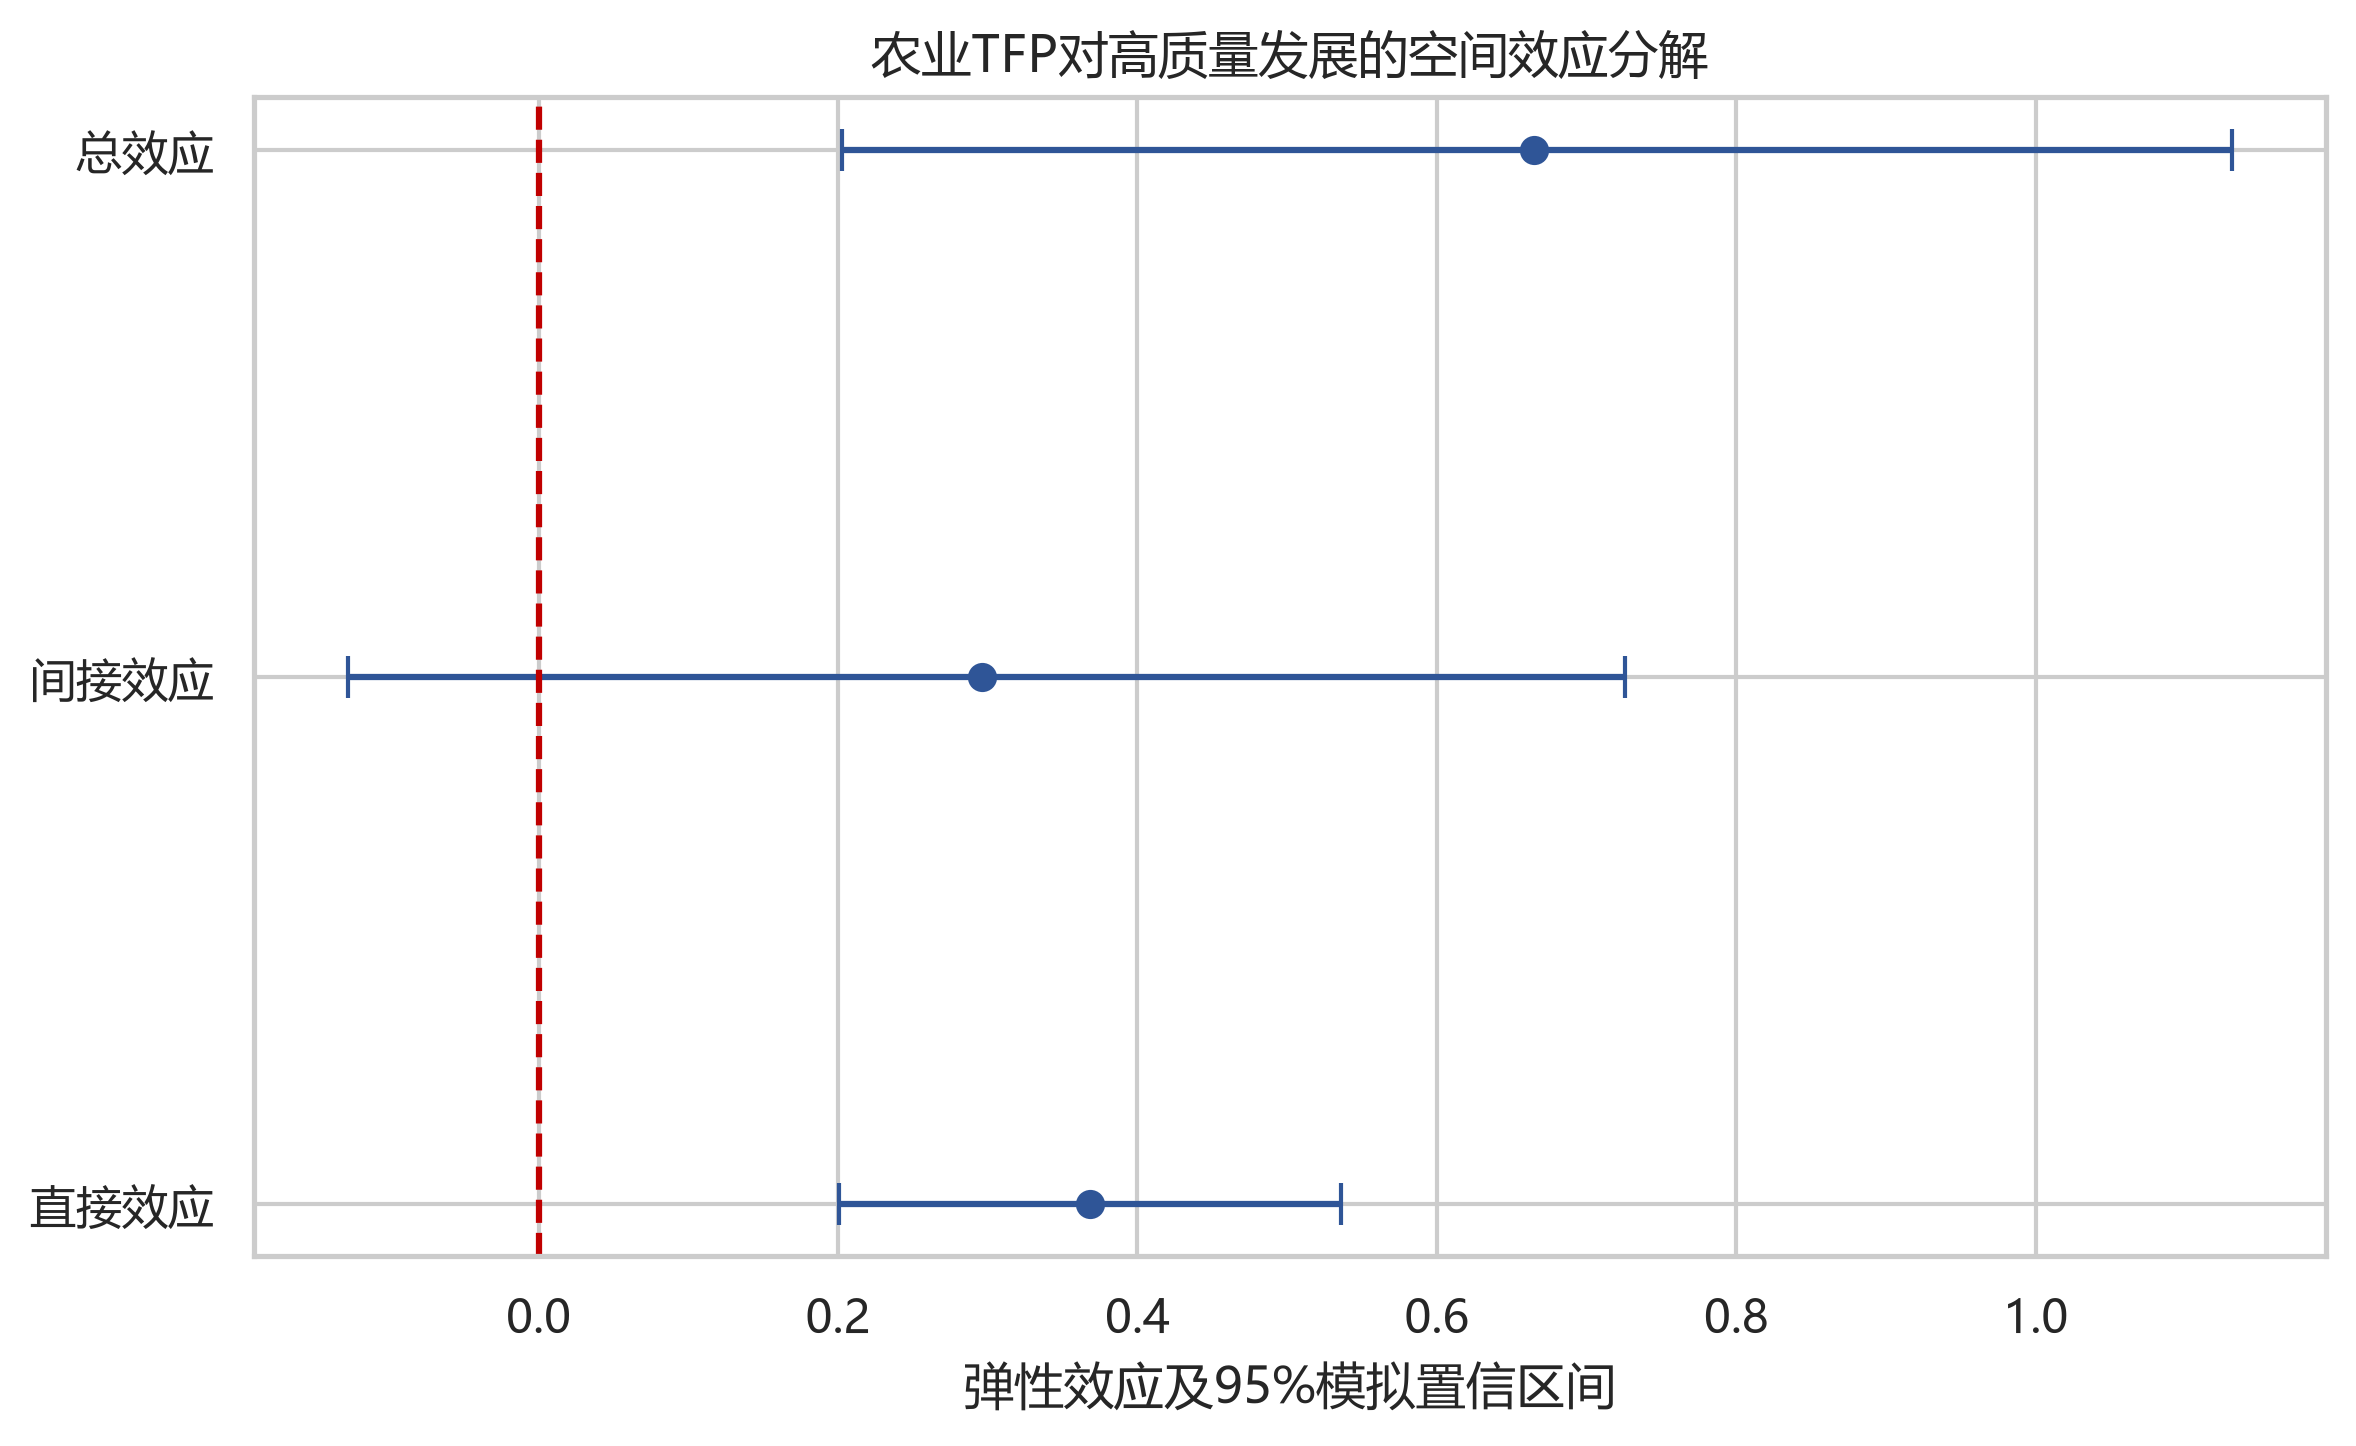
\includegraphics[width=\linewidth,height=0.82\textheight,keepaspectratio]{media/media/image23.png}
\caption*{Figure15 农业TFP对高质量发展的空间效应分解}
\end{figure}


\subsection{5.2空间门槛效应}\label{ux7a7aux95f4ux95e8ux69dbux6548ux5e94}

农业TFP能否转化为高质量发展可能取决于地区既有经济基础。本文以人均GDP的自然对数作为门槛变量，采用Hansen（1999）面板门槛方法估计单一门槛模型：

\[\ln Y_{it}=\beta_1\ln TFP_{it}\,\mathbf{1}(q_{it}\leq\gamma)+\beta_2\ln TFP_{it}\,\mathbf{1}(q_{it}>\gamma)+\delta X_{it}+\mu_i+\lambda_t+\varepsilon_{it}\]

其中q为ln(人均GDP)，γ为待估门槛。门槛值通过最小化残差平方和确定，显著性采用499次省份层面野聚类Bootstrap检验，门槛置信区间依据似然比统计量LR(γ)≤7.35确定。

\begin{longtable}[]{@{}
  >{\centering\arraybackslash}p{(\linewidth - 10\tabcolsep) * \real{0.2280}}
  >{\centering\arraybackslash}p{(\linewidth - 10\tabcolsep) * \real{0.1216}}
  >{\centering\arraybackslash}p{(\linewidth - 10\tabcolsep) * \real{0.1689}}
  >{\centering\arraybackslash}p{(\linewidth - 10\tabcolsep) * \real{0.2027}}
  >{\centering\arraybackslash}p{(\linewidth - 10\tabcolsep) * \real{0.1689}}
  >{\centering\arraybackslash}p{(\linewidth - 10\tabcolsep) * \real{0.1098}}@{}}
\caption{表9 人均GDP门槛检验及分区间效应}\tabularnewline
\toprule\noalign{}
\begin{minipage}[b]{\linewidth}\centering
\textbf{项目}
\end{minipage} & \begin{minipage}[b]{\linewidth}\centering
\textbf{ln门槛}
\end{minipage} & \begin{minipage}[b]{\linewidth}\centering
\textbf{门槛（元/人）}
\end{minipage} & \begin{minipage}[b]{\linewidth}\centering
\textbf{95\%置信区间}
\end{minipage} & \begin{minipage}[b]{\linewidth}\centering
\textbf{统计量/系数}
\end{minipage} & \begin{minipage}[b]{\linewidth}\centering
\textbf{p值}
\end{minipage} \\
\midrule\noalign{}
\endfirsthead
\toprule\noalign{}
\begin{minipage}[b]{\linewidth}\centering
\textbf{项目}
\end{minipage} & \begin{minipage}[b]{\linewidth}\centering
\textbf{ln门槛}
\end{minipage} & \begin{minipage}[b]{\linewidth}\centering
\textbf{门槛（元/人）}
\end{minipage} & \begin{minipage}[b]{\linewidth}\centering
\textbf{95\%置信区间}
\end{minipage} & \begin{minipage}[b]{\linewidth}\centering
\textbf{统计量/系数}
\end{minipage} & \begin{minipage}[b]{\linewidth}\centering
\textbf{p值}
\end{minipage} \\
\midrule\noalign{}
\endhead
\bottomrule\noalign{}
\endlastfoot
门槛检验 & 11.069 & 64171 & {[}11.044, 11.248{]} & 47.646 & 0.002 \\
低于或等于门槛 & --- & --- & --- & 0.375** & 0.036 \\
高于门槛 & --- & --- & --- & -0.344 & 0.133 \\
\end{longtable}

注：门槛显著性采用499次省份层面野聚类Bootstrap；*、**、***分别表示在10\%、5\%和1\%水平上显著。

门槛估计值为ln(人均GDP)=11.069，对应约64171元/人，原值95\%置信区间约为62537---76712元/人。SupF统计量为47.646，Bootstrap p值为0.002，拒绝不存在门槛的原假设。低门槛区间内TFP系数为0.375，在5\%水平显著为正；高门槛区间系数为－0.344，但p值为0.133，不能认为其显著为负。更稳妥的解释是：农业TFP对高质量发展的促进作用主要存在于经济基础相对较低阶段，跨过门槛后边际作用明显减弱并失去统计显著性，而不是出现确定的负向作用。H4得到非线性意义上的支持。




\begin{figure}[htbp]
\centering
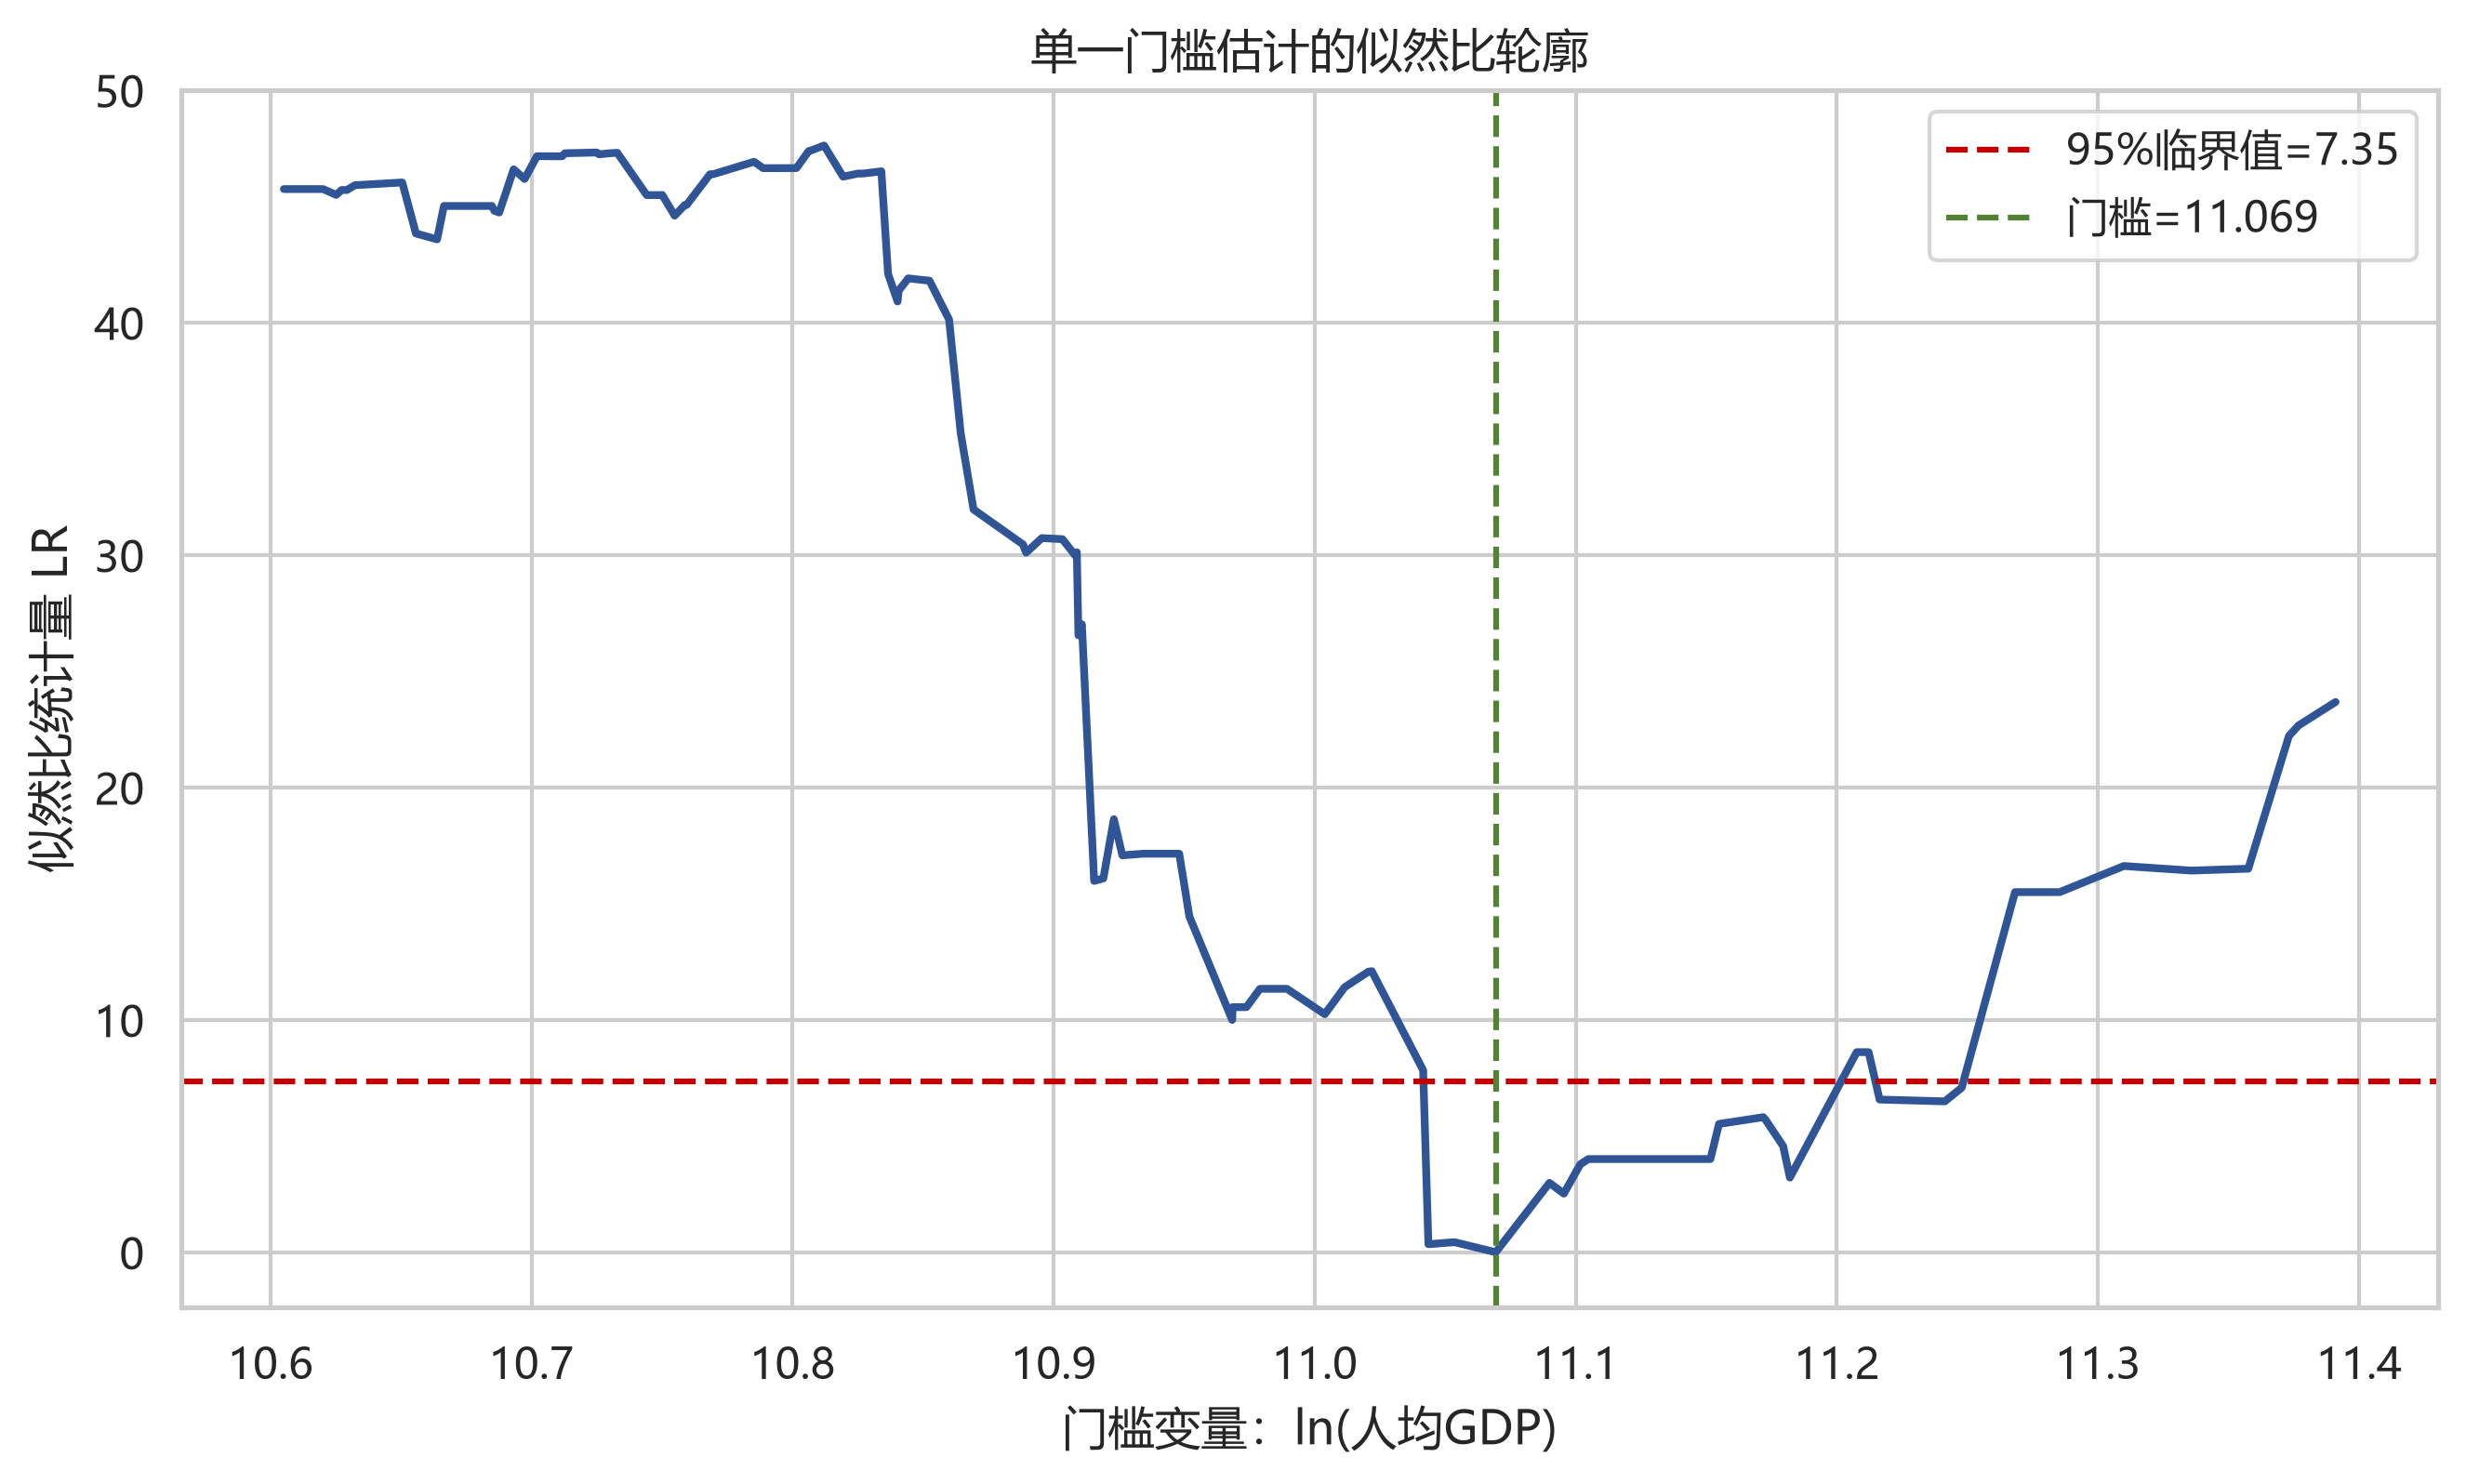
\includegraphics[width=\linewidth,height=0.82\textheight,keepaspectratio]{media/media/image24.png}
\caption*{Figure16 人均GDP门槛的似然比轮廓}
\end{figure}
\begin{figure}[htbp]
\centering
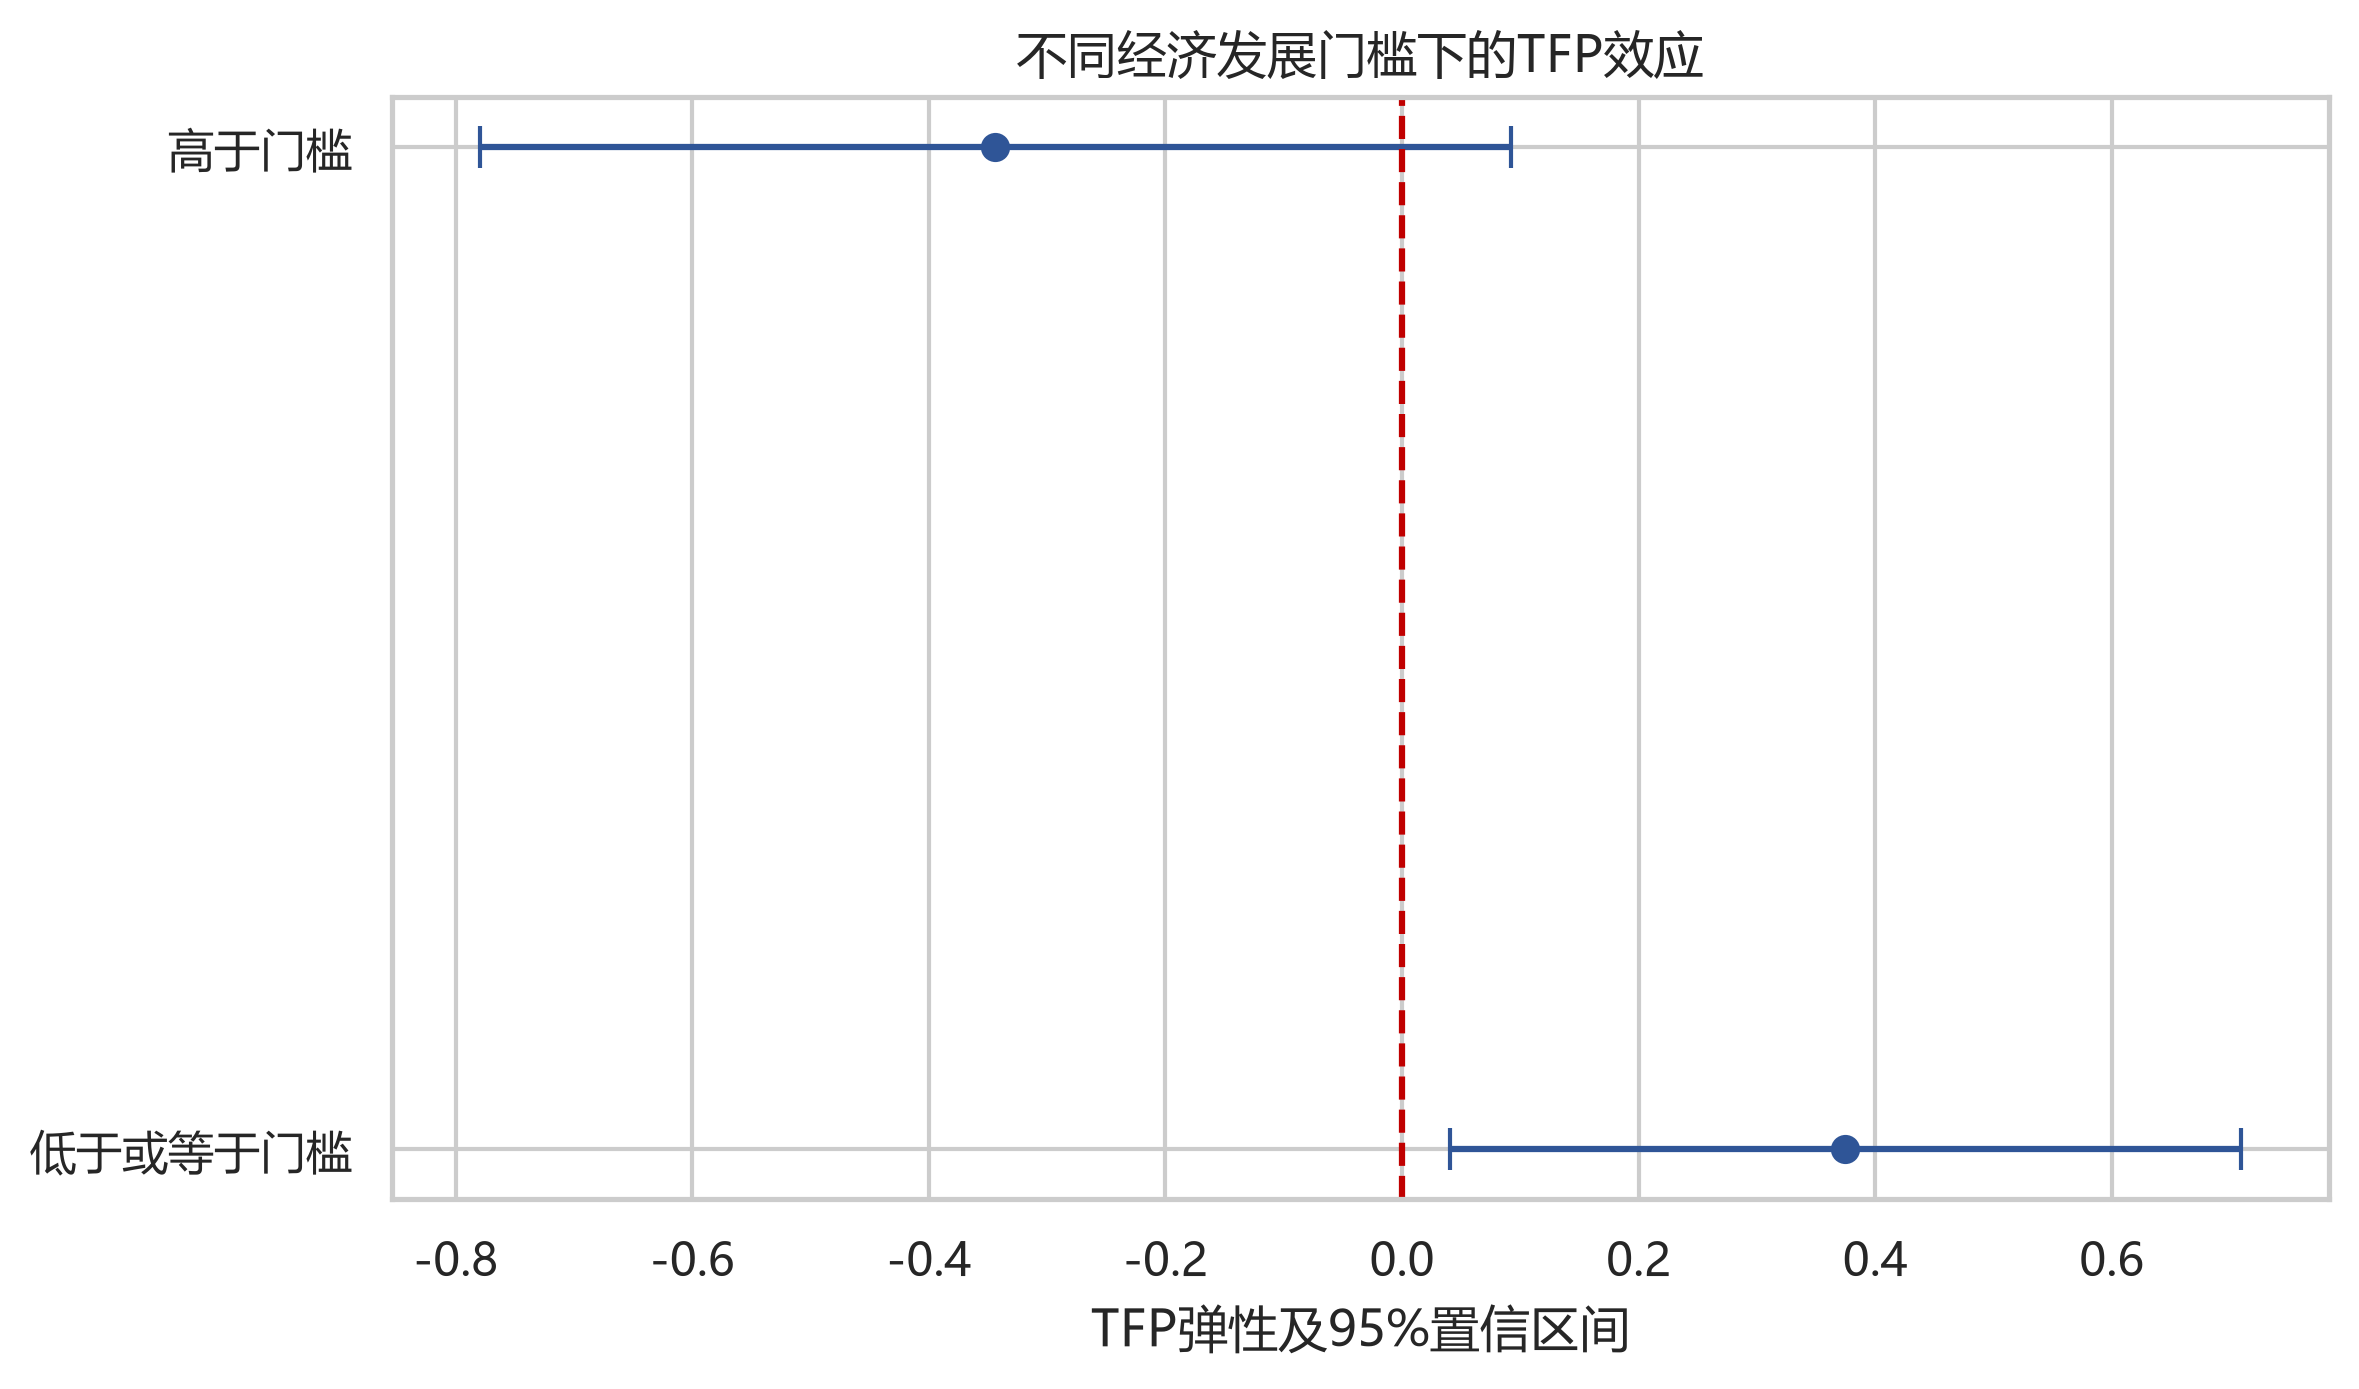
\includegraphics[width=\linewidth,height=0.82\textheight,keepaspectratio]{media/media/image25.png}
\caption*{Figure17 不同经济发展门槛下的农业TFP效应}
\end{figure}


\subsection{5.3空间马尔科夫链}\label{ux7a7aux95f4ux9a6cux5c14ux79d1ux592bux94fe}

为考察高质量发展状态的动态跃迁及其邻域依赖，本文借鉴Rey（2001）的空间马尔科夫链方法。首先按每年省际分布的四分位数将高质量发展划分为低、中低、中高和高四种相对状态，再将当期邻省加权平均水平按年度三分位数划分为低、中、高三类空间环境。无条件转移概率定义为\(p_{ij}=n_{ij}/n_i\)，空间条件转移概率则为\(p_{ij\mid c}=n_{ij\mid c}/n_{i\mid c}\)。

\begin{longtable}[]{@{}
  >{\centering\arraybackslash}p{(\linewidth - 8\tabcolsep) * \real{0.2003}}
  >{\centering\arraybackslash}p{(\linewidth - 8\tabcolsep) * \real{0.1481}}
  >{\centering\arraybackslash}p{(\linewidth - 8\tabcolsep) * \real{0.1481}}
  >{\centering\arraybackslash}p{(\linewidth - 8\tabcolsep) * \real{0.1481}}
  >{\centering\arraybackslash}p{(\linewidth - 8\tabcolsep) * \real{0.1481}}@{}}
\caption{表10 高质量发展状态的无条件转移概率}\tabularnewline
\toprule\noalign{}
\begin{minipage}[b]{\linewidth}\centering
\textbf{t期状态}
\end{minipage} & \begin{minipage}[b]{\linewidth}\centering
\textbf{低}
\end{minipage} & \begin{minipage}[b]{\linewidth}\centering
\textbf{中低}
\end{minipage} & \begin{minipage}[b]{\linewidth}\centering
\textbf{中高}
\end{minipage} & \begin{minipage}[b]{\linewidth}\centering
\textbf{高}
\end{minipage} \\
\midrule\noalign{}
\endfirsthead
\toprule\noalign{}
\begin{minipage}[b]{\linewidth}\centering
\textbf{t期状态}
\end{minipage} & \begin{minipage}[b]{\linewidth}\centering
\textbf{低}
\end{minipage} & \begin{minipage}[b]{\linewidth}\centering
\textbf{中低}
\end{minipage} & \begin{minipage}[b]{\linewidth}\centering
\textbf{中高}
\end{minipage} & \begin{minipage}[b]{\linewidth}\centering
\textbf{高}
\end{minipage} \\
\midrule\noalign{}
\endhead
\bottomrule\noalign{}
\endlastfoot
低 & 96.88\% & 3.12\% & 0.00\% & 0.00\% \\
中低 & 3.12\% & 84.38\% & 12.50\% & 0.00\% \\
中高 & 0.00\% & 10.71\% & 75.00\% & 14.29\% \\
高 & 0.00\% & 3.12\% & 9.38\% & 87.50\% \\
\end{longtable}

注：各行转移概率之和为100\%；状态按各年度省际四分位数划分。

无条件转移矩阵的主对角线概率分别为96.88\%、84.38\%、75.00\%和87.50\%，Shorrocks流动性指数仅为0.1875，说明省域高质量发展等级具有很强的路径依赖。低状态向中低状态跃迁的概率仅为3.13\%，未观察到跨越两个及以上等级的跃迁；高状态保持概率达到87.50\%。这意味着低水平省份向上流动困难，同时高水平省份具有较强稳定性。

空间条件独立性检验的G统计量为21.758，999次置换p值为0.087，在10\%水平上呈边际显著、但未通过5\%检验。因此邻域环境对状态转移具有提示性而非强证据。具体看，中低状态在高邻域环境下向中高状态跃迁的概率为33.33\%，高于低邻域和中邻域下的7.69\%；中高状态在高邻域环境下向高状态跃迁的概率为22.22\%，也高于低邻域下的0。这与正向空间关联相符，但部分条件单元样本很少，应避免过度解释。总体上，H5关于等级锁定得到较强支持，邻域条件效应仅得到弱支持。




\begin{figure}[htbp]
\centering
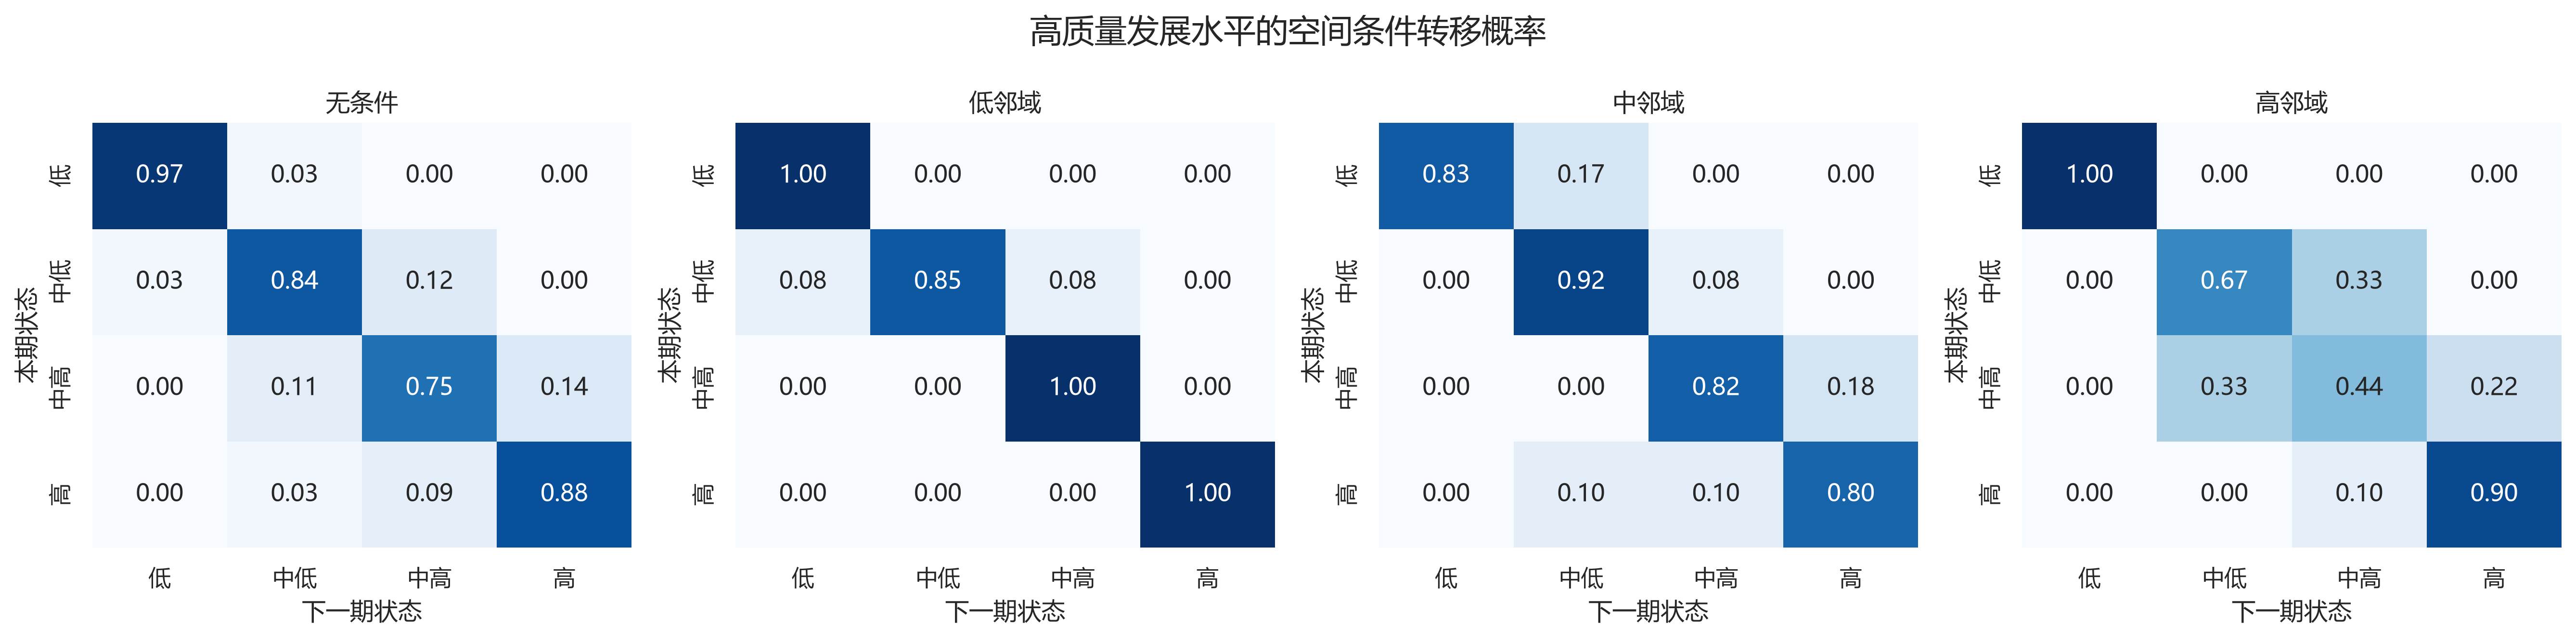
\includegraphics[width=\linewidth,height=0.82\textheight,keepaspectratio]{media/media/image26.png}
\caption*{Figure18 高质量发展水平的空间条件转移矩阵}
\end{figure}
\begin{figure}[htbp]
\centering
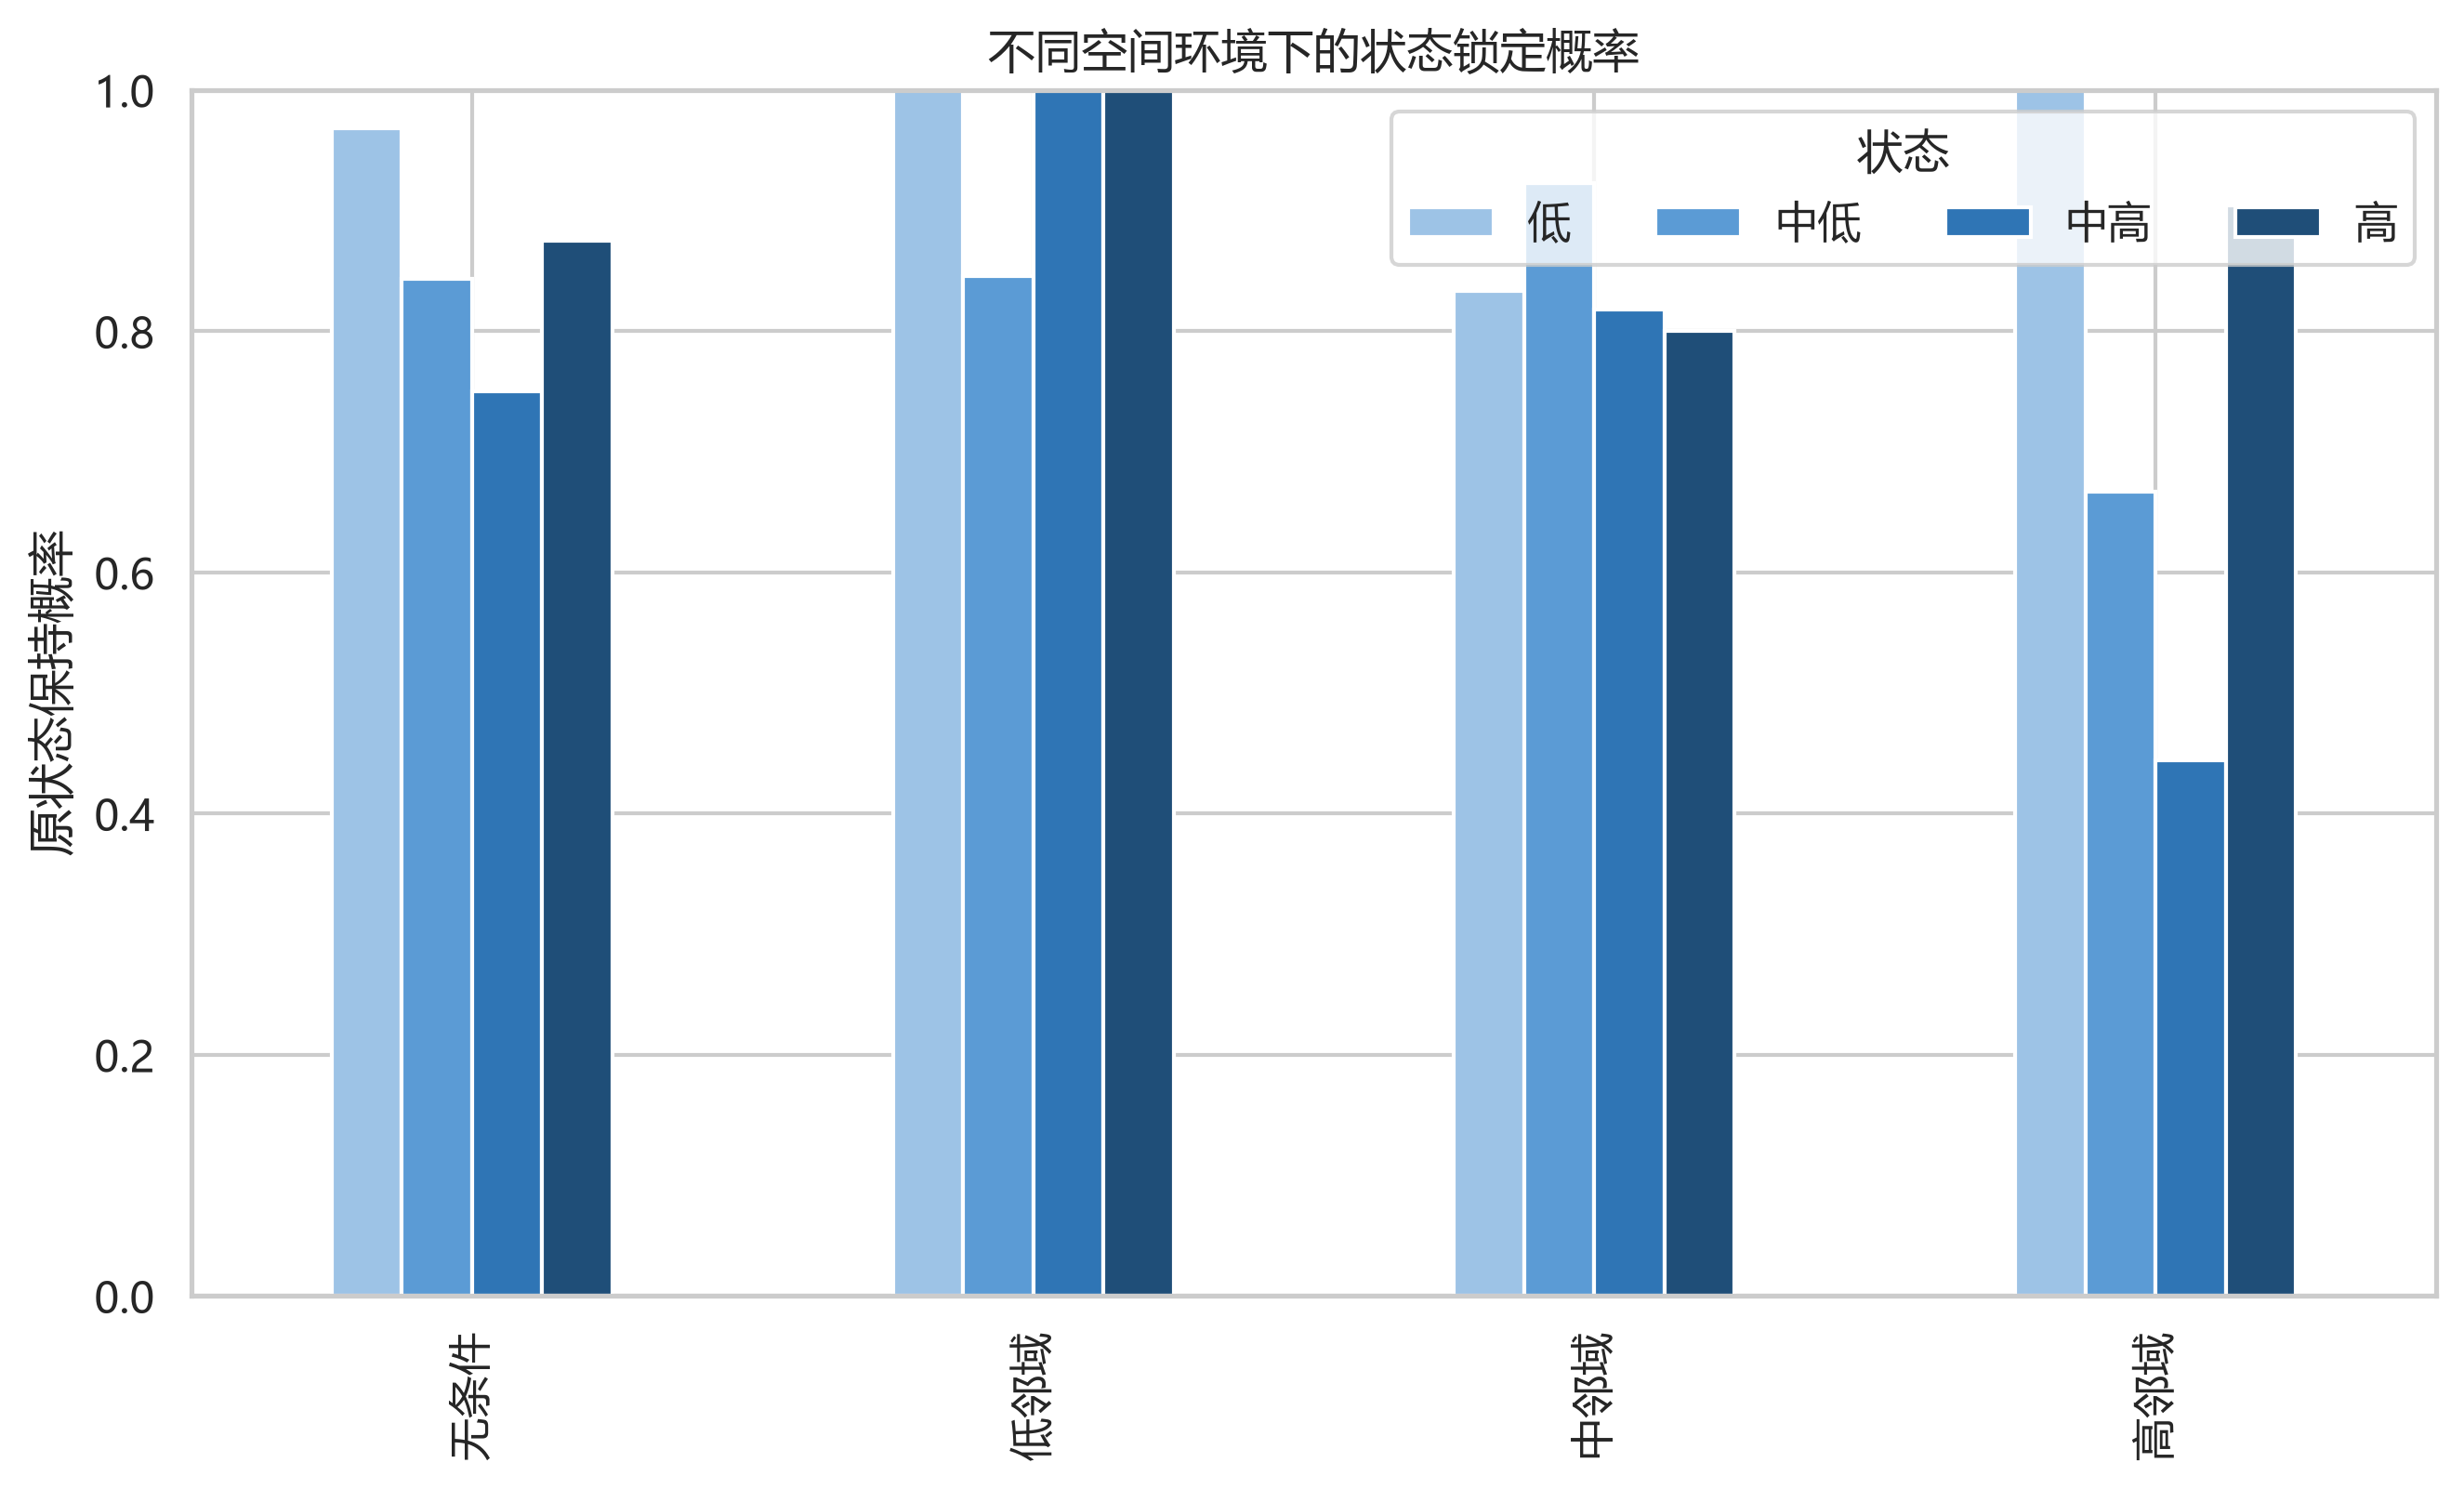
\includegraphics[width=\linewidth,height=0.82\textheight,keepaspectratio]{media/media/image27.png}
\caption*{Figure19 不同空间环境下的状态锁定概率}
\end{figure}


\section{6讨论与不足}\label{ux8ba8ux8bbaux4e0eux4e0dux8db3}

本文基于2016---2020年31个省级行政区平衡面板，从分布演变、区域差异、空间依赖、非线性和动态跃迁等维度考察农业TFP与经济高质量发展的关系。研究发现，高质量发展指数在样本期内整体上升且省际差异收敛，而累计农业TFP虽然总体提高，但其省际差异持续扩大。二者呈现不同的分布演进方向，说明农业生产率增长并不会机械地、同步地转化为综合高质量发展。

Dagum分解表明，高质量发展差异主要来自东中西部之间的净差异，但区域间差距呈缩小趋势；累计TFP的区域间净差异则逐渐扩大，且西部内部差异增长明显。这意味着部分西部省份的TFP追赶并不代表整个西部形成同步提升，更可能体现为少数省份的前沿移动、投入收缩或低基期下的累计放大。区域政策因而应从追求单一生产率增速转向提高生产率成果向居民福利、绿色转型、城乡协调和公共服务的转化效率。

空间分析显示，高质量发展具有稳定的正空间相关，长三角形成较连续的高值集聚，部分西部省份表现为低值集聚。空间杜宾模型进一步表明，高质量发展本身存在显著正向空间联动，但农业TFP的间接效应未达到常用显著性水平。由此可见，邻近地区的发展基础、公共治理和市场联系可能具有协同作用，但农业技术效率能否跨省外溢仍取决于技术扩散渠道、要素流动和区域吸收能力。政策上应强化跨区域农技推广、农业社会化服务和基础设施互联，而不能将一般空间相关直接等同于生产率溢出。

门槛结果显示，当人均GDP低于约6.42万元时，TFP提高对高质量发展具有显著促进作用；超过门槛后，估计效应转负但不显著。该结果更符合边际作用递减而非显著负效应：在经济基础较低地区，农业仍占据重要地位，生产率改善能够释放劳动力、提高农业收入并改善资源配置；在较高发展阶段，高质量发展的主要约束可能转向创新能力、现代服务业、生态治理与公共服务，单纯依靠农业TFP难以继续形成同等强度的推动。

空间马尔科夫结果揭示了较强的等级锁定：四类状态的保持概率均较高，低水平省份向上跃迁尤其困难。邻域环境对转移概率仅在10\%水平呈边际显著，说明空间环境可能影响跃迁机会，但在短样本下证据仍有限。对于长期处于低值集聚的地区，应通过跨区域基础设施、公共服务均等化、人才和技术流动打破低水平空间均衡；对于高值集聚地区，则需要发挥示范扩散和产业链带动作用。

本文仍存在若干局限。第一，样本仅覆盖2016---2020年，时间维度较短，难以充分识别长期动态、结构突变和政策冲击。第二，DEA---Malmquist投入受数据可得性限制，尚未纳入土地和劳动等核心要素，产出使用当年价农林牧渔业总产值，可能同时受到价格变化和统计口径调整影响。第三，累计TFP以2016年为共同基期，后期差异具有机械累积性质，因此其基尼系数与马尔科夫结果不能解释为绝对生产率水平。

第四，空间权重采用省级接壤矩阵，并将海南与广东桥接，尚未同时考察地理距离、经济距离、交通联系和贸易网络等替代权重。第五，内生性检验使用一期滞后内部工具变量，虽然第一阶段较强，但排除限制无法完全验证，结论仍不能等同于严格因果效应。第六，门槛、局部Moran和空间马尔科夫条件矩阵在31省、5年样本下存在小样本不确定性，多重局部检验也可能增加偶然显著概率。未来研究可扩展更长时期数据，使用价格平减后的农业产出，补充土地、劳动和气候投入，引入历史农业禀赋、政策试点或外生气候冲击等更有说服力的工具变量，并在动态空间面板及多重空间权重下检验结论稳健性。

\section{引用}\label{ux5f15ux7528}

\textbf{《经济日报》. 2023.} 深刻把握经济高质量发展的内涵要义. 2023.

\textbf{陈景华, 陈妩 和 陈敏敏. 2020.} 中国经济高质量发展水平、区域差异及分布动态演进. 数量经济技术经济研究. 2020年.

\textbf{陈诗一，陈登科. 2018.} 雾霾污染、政府治理与经济高质量发展. 经济与管理科学. 2018年.

技术效率、技术进步与中国农业全要素生产率的提高------基于国际比较的实证分析. \textbf{车维汉杨荣. 2010.} 3, 上海~: 上海财经大学出版社, 2010年, 卷 36. DOI:10.16538/j.cnki.jfe.2010.03.005.

科技金融、经营主体活力与经济高质量发展. \textbf{蔡文心杜旭虹,张洪胜,武鑫,张宛玲. 2026.} 北京~: 经济与管理科学, 2026年.

绿色技术创新对农业绿色全要素生产率影响的异质性与机制研究. \textbf{曹先磊左恒源. 2026.} 长沙~: 科学出版社, 2026年. https://doi.org/10.13872/j.1000-0275.2025.0488..

\textbf{蒲晓晔 和 FidrmucJarko{[}奥{]}. 2018.} 中国经济高质量发展的动力结构优化机理研究. 西北大学学报(哲学社会科学版). 2018年.

\textbf{赵丽芳代文涛,孙洪杰. 2026.} 政策跟踪审计与城市经济高质量发展------基于空间面板杜宾模型的实证研究. 审计与经济研究. 2026年.

\textbf{赵涛张智,梁上坤. 2020.} 数字经济、创业活跃度与高质量发展------来自中国城市的经验证据. 经济与管理科学. 2020年, 卷 36, 10.

中国省际经济高质量发展的测度与分析. \textbf{陈博、任保平. 2018年.} 2018年年.
\end{document}
